%%
%% This is file `sample-sigconf-authordraft.tex',
%% generated with the docstrip utility.
%%
%% The original source files were:
%%
%% samples.dtx  (with options: `all,proceedings,bibtex,authordraft')
%% 
%% IMPORTANT NOTICE:
%% 
%% For the copyright see the source file.
%% 
%% Any modified versions of this file must be renamed
%% with new filenames distinct from sample-sigconf-authordraft.tex.
%% 
%% For distribution of the original source see the terms
%% for copying and modification in the file samples.dtx.
%% 
%% This generated file may be distributed as long as the
%% original source files, as listed above, are part of the
%% same distribution. (The sources need not necessarily be
%% in the same archive or directory.)
%%
%%
%% Commands for TeXCount
%TC:macro \cite [option:text,text]
%TC:macro \citep [option:text,text]
%TC:macro \citet [option:text,text]
%TC:envir table 0 1
%TC:envir table* 0 1
%TC:envir tabular [ignore] word
%TC:envir displaymath 0 word
%TC:envir math 0 word
%TC:envir comment 0 0
%%
%%
%% The first command in your LaTeX source must be the \documentclass
%% command.
%%
%% For submission and review of your manuscript please change the
%% command to \documentclass[manuscript, screen, review]{acmart}.
%%
%% When submitting camera ready or to TAPS, please change the command
%% to \documentclass[sigconf]{acmart} or whichever template is required
%% for your publication.
%%
%%


\documentclass[sigconf]{acmart}

\copyrightyear{2025}
\acmYear{2025}
\setcopyright{acmlicensed}
\acmConference[WWW '25] {Proceedings of the ACM Web Conference 2025}{April 28--May 2, 2025}{Sydney, NSW, Australia.}
\acmBooktitle{Proceedings of the ACM Web Conference 2025 (WWW '25), April 28--May 2, 2025, Sydney, NSW, Australia}
\acmISBN{979-8-4007-1274-6/25/04}
\acmDOI{10.1145/3696410.3714617}
% 1 Authors, replace the red X's with your assigned DOI string during the rightsreview eform process.
% 2 Your DOI link will become active when the proceedings appears in the DL.
% 3 Retain the DOI string between the curly braces for uploading your presentation video.

\settopmatter{printacmref=true}




\usepackage{graphicx}
\usepackage{enumitem}
\usepackage{multirow} 
\usepackage{fancyhdr}
\usepackage{caption}
\pagestyle{empty}
\usepackage{array}
\usepackage{xcolor}
\newcolumntype{B}{>{\columncolor{blue!10}\bfseries\color{blue}}c}
\usepackage{bm}
\usepackage{colortbl}
\usepackage{threeparttable}
\usepackage{afterpage}
\usepackage{pgfplots}  
\usepackage{tablefootnote}
\usepackage{amsmath}
\usepackage{tikz}
\usepackage{pgfplots}
\usepackage{graphicx}
\usepackage{subcaption}
\usepackage{subcaption}
\usepackage{pgfplotstable}  
\usepackage{graphicx}  
\usepackage{adjustbox}
\usepackage{setspace} 
% 定义颜色映射,这里使用红色渐变  
\pgfplotsset{  
    colormap={gray}{  
        color(0)=(white);  
        color(1)=(black)  
    }  
}  
\captionsetup[subfigure]{justification=centering}
\usetikzlibrary{shadows}
% 推荐使用的包
% \usepackage{scalefnt} %用于设置字体
% \usepgfplotslibrary{fillbetween}
% \usepackage{tgtermes}

\definecolor{lightblue}{rgb}{0.94, 0.94, 1}
\definecolor{lightorange}{rgb}{1, 0.99, 0.93}
\definecolor{lightpink}{rgb}{1, 0.93, 0.93}
\definecolor{lightgreen}{rgb}{0.92, 0.98, 0.92}

\newcommand{\colorrect}[1]{\textcolor{#1}{\ding{110}}}


% 预先定义一些colors
\definecolor{color1}{RGB}{120,159,124}
\definecolor{color2}{RGB}{199,115,100}
\definecolor{color3}{RGB}{252,104,58}
\definecolor{color4}{RGB}{250,168,68}
\definecolor{color5}{RGB}{121,137,184}
\definecolor{color6}{RGB}{167,98,236}
\definecolor{color8}{RGB}{137,137,137}%%灰色
\definecolor{color9}{RGB}{90,82,252}
%%
%% end of the preamble, start of the body of the document source.
\begin{document}

%%
%% The "title" command has an optional parameter,
%% allowing the author to define a "short title" to be used in page headers.
% \title{Sherlock: Towards Multi-scene Video Abnormal Event Extraction and Localization via a Global-local Spatial-senstive LLM}



\title[Sherlock]{\texorpdfstring{\begin{minipage}[b]{0.01\textwidth}
  \raisebox{1mm}{\includegraphics[scale=0.145]{image/logo.png}}
\end{minipage}\hspace{10mm}%
\begin{minipage}[b]{0.89\textwidth}
\begin{center}
   Sherlock: Towards Multi-scene Video Abnormal Event Extraction and Localization via a Global-local Spatial-sensitive LLM
\end{center}
\end{minipage}}{}}

%%
%% The "author" command and its associated commands are used to define
%% the authors and their affiliations.
%% Of note is the shared affiliation of the first two authors, and the
%% "authornote" and "authornotemark" commands
%% used to denote shared contribution to the research.

\author{Junxiao Ma}
\email{jxma0711@stu.suda.edu.cn}
\affiliation{
  \institution{School of Computer Science and Technology, Soochow University}
  \city{Suzhou}
  \country{China}
}

\author{Jingjing Wang}
\authornote{Corresponding Author: Jingjing Wang.}
\email{djingwang@suda.edu.cn}
\affiliation{
  \institution{School of Computer Science and Technology, Soochow University}
  \city{Suzhou}
  \country{China}
}


\author{Jiamin Luo}
\email{20204027003@stu.suda.edu.cn}
\affiliation{
  \institution{School of Computer Science and Technology, Soochow University}
  \city{Suzhou}
  \country{China}
}

\author{Peiying Yu}
% \authornote{equal contribution}
\email{20244227007@stu.suda.edu.cn}
\affiliation{
  \institution{School of Computer Science and Technology, Soochow University}
  \city{Suzhou}
  \country{China}
}

\author{Guodong Zhou}
\email{gdzhou@suda.edu.cn}
\affiliation{
  \institution{School of Computer Science and Technology, Soochow University}
  \city{Suzhou}
  \country{China}
}
%%
%% By default, the full list of authors will be used in the page
%% headers. Often, this list is too long, and will overlap
%% other information printed in the page headers. This command allows
%% the author to define a more concise list
%% of authors' names for this purpose.
\renewcommand{\shortauthors}{Junxiao Ma, Jingjing Wang, Jiamin Luo, Peiying Yu \& Guodong Zhou}

%%
%% By default, the full list of authors will be used in the page
%% headers. Often, this list is too long, and will overlap
%% other information printed in the page headers. This command allows
%% the author to define a more concise list
%% of authors' names for this purpose.

%%
%% The abstract is a short summary of the work to be presented in the
%% article.
\begin{abstract}
Retrieval-Augmented Generation (RAG) is often used with Large Language Models (LLMs) to infuse domain knowledge or user-specific information. In RAG, given a user query, a retriever extracts chunks of relevant text from a knowledge base. These chunks are sent to an LLM as part of the input prompt. Typically, any given chunk is repeatedly retrieved across user questions. However, currently, for every question, attention-layers in LLMs fully compute the key values (KVs) repeatedly for the input chunks, as state-of-the-art methods cannot reuse KV-caches when chunks appear at arbitrary locations with arbitrary contexts. Naive reuse leads to output quality degradation.  This leads to potentially redundant computations on expensive GPUs and increases latency. In this work, we propose \sys, a system for managing and reusing precomputed KVs corresponding to the text chunks (we call \textit{chunk-caches}) in RAG-based systems. We present how to identify \hl{\textit{chunk-caches} that are reusable}, how to efficiently perform a small fraction of recomputation to \textit{fix} the cache to maintain output quality, and how to efficiently store and evict \textit{chunk-caches} in the hardware for maximizing reuse while masking any overheads. With real production workloads as well as synthetic datasets, we show that \sys reduces redundant computation by \textbf{51\%} over SOTA prefix-caching and \textbf{75\%} over full recomputation.
\hl{Additionally, with continuous batching on a real production workload, we get a \textbf{1.6$\times$} speedup in throughput and a \textbf{2$\times$} reduction in end-to-end response latency over prefix-caching while maintaining quality, for both the \llama-3-8B and \llama-3-70B models. 
}
\end{abstract}






%%
%% The code below is generated by the tool at http://dl.acm.org/ccs.cfm.
%% Please copy and paste the code instead of the example below.
%%

\begin{CCSXML}
<ccs2012>
   <concept>
       <concept_id>10010147.10010178</concept_id>
       <concept_desc>Computing methodologies~Artificial intelligence</concept_desc>
       <concept_significance>500</concept_significance>
       </concept>
 </ccs2012>
\end{CCSXML}

\ccsdesc[500]{Computing methodologies~Artificial intelligence}
%%
%% Keywords. The author(s) should pick words that accurately describe
%% the work being presented. Separate the keywords with commas.

\keywords{Multi-scene Video, Video Abnormal Event, Spatial-sensitive LLM}
%% A "teaser" image appears between the author and affiliation
%% information and the body of the document, and typically spans the
%% page.
\begin{teaserfigure}
\vspace{-0.3 cm}
\setlength{\abovecaptionskip}{0.5 ex}
% \setlength{\belowcaptionskip}{-1 ex}
  \includegraphics[width=\textwidth]{image/abstract.pdf}
  \caption{(a) and (b) illustrate two surveillance video examples for our M-VAE task and Sherlock model in two scenes (Street and Residence). Sherlock precisely generates the abnormal event quadruples and their corresponding timestamps. (c) presents a circular ratio diagram illustrating different spatial information. From (c), we observe that the global spatial information and the local spatial information (i.e., action, object relation, and background) in our M-VAE dataset are imbalanced.}
  \label{fig:abstract}
\end{teaserfigure}

% \received{20 February 2007}
% \received[revised]{12 March 2009}
% \received[accepted]{5 June 2009}

%% This command processes the author and affiliation and title
%% information and builds the first part of the formatted document.
\maketitle
\documentclass[../main.tex]{subfiles}
\graphicspath{{../images/}}
\makeatletter
\def\input@path{{../images/}}
\makeatother
\begin{document}
\section{Introduction}
\begin{figure}
\centering
\begin{tikzpicture}
\node[inner sep=0pt] (ws) at (0, 0) {
\includegraphics[height=.4\textwidth, trim={10cm 0 10cm 0},clip]{world_space.png}};
\node[inner sep=0pt] (cs) at (6,0) {\includegraphics[height=.4\textwidth, trim={10cm 1cm 10cm 4cm},clip]{conf_space.png}};
\end{tikzpicture}
\vspace{-5pt}
\label{fig:pbrm_intro}
\caption{\textbf{Left}: Shows world space obstacles as grey spheres. Robots start and goal configuration is colored red and green, respectively. Configurations along the computed path are colored transparent blue. \textbf{Right:} Mapped world space scenario to configuration space. Obstacle region is the grey mesh. Red spheres are collision-free regions computed by the neural SCDF. The optimized shortest path in the convex corridor is the blue curve.}
\vspace{-25pt}
\end{figure}
Motion planning is the problem of finding a collision-free trajectory that connects a given start and goal configuration. The planning takes place in the configuration space of the robot. For single body robots, like mobile robots or drones, the configuration space and the world space are usually the same. This simplifies the planning, since explicit obstacle representations are available which enables geometrical tools like separating hyperplanes, smallest distance to obstacles etc., to be used when designing motion planning algorithms. For multi-body robots like manipulators, the situation is completely different. The world space obstacles are usually mapped to non-convex regions, and to make the problem even harder, the mapping is usually not known. Forming explicit representations of the obstacle region in the configuration space is usually too expensive or intractable. Despite all of this, sampling based planners are used with great success, which mainly is due to their use of implicit representations of the obstacle region. The basic idea is to construct a graph in the configuration space that covers and connects the collision-free region. From this graph, a path can be extracted that connects a given start and goal configuration. The approach is computationally expensive, since the graph is constructed with the smallest geometrical building block available, points, which represents a collision-check. Furthermore, the extracted paths from the graph are non-smooth and jagged due to the stochastic nature of the approach. This adds an additional post-processing step to the process, where the paths are shortcutted and smoothened, before the path can be used for tracking. Clearly a lot of time is invested to form this graph and produce smooth paths. Thus, if the obstacles start to move, then all of this work is done in no use, since all points that make up this graph need to be re-verified, which is simply too time consuming to be done in real time.
\\\\
In this work, we want to address the existing drawbacks of the sampling based planners. Our main contribution is an improved motion planner where each vertex in the graph covers a collision-free region in the form of a sphere instead of a point and where the edges are formed with neighboring intersecting spheres. This representation has the advantage of instead of returning piecewise linear paths, returning a sequence of overlapping spheres, i.e. a convex corridor, that connects a given start and goal configuration, illustrated in Figure \ref{fig:pbrm_intro}. This convex corridor allows us to use convex optimization to produce smooth trajectories, instead of computationally expensive post-processing methods. The representation further allows us to estimate the coverage of the collision-free space, which gives us awareness and feedback in the offline roadmap construction phase. Finally, our representation is simple to adapt to moving obstacles, simply requery for the new radii and recheck for intersections. 
\\\\
The spherical collision-free regions are formed using a signed distance function (SDF), which is a function that returns the smallest distance from an arbitrary point to the boundary of an obstacle. As the name implies, the distance is signed, thus if the point is inside the obstacle it is negative otherwise positive. If the distance is positive, a sphere with radius equal to the distance is guaranteed to cover a collision-free region. Using an SDF in motion planning is not new, but what is novel about our approach is that we express the distance in the configuration space instead of the world space and by doing so allows us to form these convex collision-free regions. We refer to the resulting SDF as a signed configuration distance function (SCDF). Computing an SCDF analytically is non-trivial, our approach is therefore to parameterize the SCDF with a deep neural network and learn the mapping by supervised learning. Our resulting neural SCDF can compute distances for different parameter values of obstacle shapes and we also show how multiple distances can be combined, thus making our approach flexible.
\section{Related work}
Motion planning algorithms can roughly be divided into three families, grid-based, sampling based and optimization based methods. Grid-based methods (GBM) discretize the planning space from which a graph is then compiled. A standard search method is A$^\star$ \citep{a_star}, which is classified as an \textit{informed} search method, since it employs a heuristic function to speed up the search. A$^\star$ guarantees to return an optimal path at the level of discretization used. GBMs usually discretize the planning space by a regular lattice and this limits the GBMs to problems with low dimensionality due to the curse of dimensionality. Thus, GBMs are usually limited to single-body robots where the degrees of freedom (DOF) are low. To overcome the inherent scaling problem with the GBMs, stochastic methods are usually used for multi-body robots. These methods are termed as sampling-based methods (SBM) and core members within this family are the rapidly-exploring random trees (RRT) \citep{rrt} and the probabilistic roadmap (PRM) \citep{prm}. RRT grows a tree from the start configuration and explores the collision-free region in a rapid way until it is able to connect to the goal region. RRT is usually improved by bi-directional planning \citep{rrt_connect}, i.e. an additional tree is grown from the goal configuration and the trees are tested for connection after any tree has been expanded. RRT is a single-query method, thus it searches for a path from scratch each time it is queried. Contrary to this, PRM is a multi-query method, which solves for multiple queries without starting from scratch. PRM does this by creating a roadmap (graph) that covers the collision-free space as an offline step. The graph is then used to solve for multiple queries. PRMs are used in cases where the environment does not change since the extra offline step is too computationally costly and needs to be re-done if the environment is changed. In our work, we address this inherent issue by using a different roadmap representation. Our vertices in the graph cover a collision-free region in the form of spheres and we form the edges by checking for intersecting spheres. If something in the environment changes, we recompute the spheres radii and recheck the intersections, without relying on collision detection. We use a trained neural network to compute the sphere radius, therefore querying for the radius can be done fast, hence our representation enables the PRM for dynamic environments.
\\\\
In the recent decades, optimization based methods (OBM) \citep{chomp, schulman, itomp, stomp} have been introduced as an alternative to SBM for multi-body robots. Like the SBM, the OBMs scale well to higher dimensional problems and produce smoother motion. It is common to use a SDF in the optimization since it is a smooth function, thus enabling gradient-based methods. However, the standard way of expressing the SDF is in world space. The distance therefore needs to be mapped to the configuration space by the forward kinematics. This mapping makes the optimization problem a non-linear program (NLP), which is computationally expensive to solve. Recently, a different approach has been proposed. In \cite{mp_gcs} motion planning is formulated as a convex optimization problem by using the graph of convex sets framework \citep{gcs}. The underlying idea is to decompose the collision-free space into intersecting convex sets from which a convex optimization problem is formulated. In cases where an explicit representation of the obstacles in the configuration space exists, like for single-body robots, creating collision-free convex regions can be done fast \citep{iris}. For multi-body robots, this is non-trivial. Existing work does this successfully \citep{iris_nlp, iris_c} by an optimization based approach, but the methods are still too time consuming to be used in the presence of moving obstacles. Our approach is instead to use deep learning to learn an SDF expressed in the configuration space. With this, we can query for shortest distances to the collision boundary, which allows us to expand spherical regions which are collision-free. Our approach is fast and therefore enables our suggested roadmap planner to be used in dynamic environments.
\\\\
Recent research has focused on learning collision detection \citep{fk_kernel_distance, diffco, graphdistnet} by predicting the signed distance between the robot links and the surrounding obstacles in the world space. The learned SDF is used in trajectory optimization but since the distance is expressed in the world space, the problem becomes an NLP and therefore takes a long time to solve. We take a novel approach and suggest to instead express the signed distance in the configuration space. This allows us to improve the PRM at the same time as it enables convex optimization for trajectory optimization, which runs faster and is more reliable than NLP solvers. In \cite{cspf} a learned signed distance function in the configuration space is proposed similar to our approach. However, their approach is restricted to point cloud representations, while we propose to represent the obstacles as parameterized geometric shapes, e.g. spheres. Furthermore, we also show how to use our learned SCDF to improve an existing roadmap planner.
\section{Problem formulation}
A robot is located in the world space, $\W \subset \R^3 $. The unique location of the robot is given by its configuration $\q \in \C$, where $\C$ is the configuration space. The set of points covered by the robots bodies at a certain configuration is expressed as $\B(\q) \subset \W$. The robot is surrounded by $\NrObst$ obstacles $\O = \bigcup_{i=1}^{\NrObst} \O_i$, where  $\O_i \subset \W$. The representation of the obstacle in the configuration space is the set $\C\O_i = \{\q \in \C \: |\: \B(\q) \cap \O_i \neq \emptyset \}$. The obstacle space is formed as $\Co = \bigcup_{i=1}^{\NrObst} \C \O_i$. The complement is referred to as the free space, $\Cf = \C \setminus \Co$. The path planning problem is a tuple, ($\Cf$, $\qStart$, $\qGoal$), where we want to connect a query pair, consisting of a start, $\qStart$, and goal configuration, $\qGoal$, with a geometric path, $\q(s): [0, 1] \mapsto \Cf$, such that $\q(0)=\qStart$ and $\q(1)=\qGoal$, or report correctly when such a path does not exist.
\end{document}

\begin{figure*}[t]
\vspace{-0.3cm}
\setlength{\abovecaptionskip}{0.5 ex}
\setlength{\belowcaptionskip}{-3 ex}
  \centering
  \includegraphics[width=\textwidth]{image/model.pdf}
  \centering
  \caption{The overall framework of Sherlock. It consists of a Global-local Spatial-enhanced MoE (GSM) Module and a Spatial Imbalance Regulator (SIR). The SIR exerts a direct influence on the output weights of the expert gate.}
  \Description{our method xxx}
  \label{fig:model}
\end{figure*}
\section{Related Work}
% \subsection{Vision Language Model}
% 시각장애인에서 상황을 설명할 DB가 없으니 만들었다. 그리고 이를 VLM에 튜닝했다.
\subsection{Technical approaches for assisting the visually-impaired}


\subsection{Datasets for visual instruction tuning}

\section{Methodology}
\label{sec:approach}

\begin{figure}[!t]
\centering
\includegraphics[width=0.5\textwidth]{Pipeline.png}
\caption{Workflow. For each synthesis or sketching task, we create an input query for the LLM such that the query contains the target property in natural language or Alloy (depending on the kind of task), run the query, get the LLM's output, and use the Alloy analyzer to validate it with respect to a reference (ground truth) formula.}
\label{fig:workflow}
\end{figure}

We consider the following three methods for employing large language models (LLMs) to create Alloy formulas to investigate the capabilities and limitations of LLMs in writing Alloy:

\begin{enumerate}
\item
{\bf English to Alloy}. We employ LLMs to write complete Alloy formulas in multiple different ways from given natural language descriptions (in English);
\item
{\bf Alloy to Alloy}. We employ LLMs to create multiple alternative but equivalent formulas in Alloy with respect to given formulas in Alloy; and
\item
{\bf Sketch to Alloy}. We employ LLMs to complete sketches~\cite{SolarLazemaPhD2008,WangETALABZ2018ASketch} of Alloy
formulas and populate the holes in the sketches by synthesizing Alloy
expressions and operators so that the completed formulas accurately
represent the desired properties (that are given in natural language).  \end{enumerate}

\begin{table}[!t]
\begin{tabular}{r@{\hskip 0.2cm}|l|p{4cm}|p{5cm}}
& \multicolumn{1}{c|}{\Intro{Property}} & \multicolumn{1}{c|}{\Intro{Natural language desc.}} & \multicolumn{1}{c}{\Intro{Reference Alloy formula}}\\
\hline
1 & DAG & Directed acyclic graph &
\begin{lstlisting}[style=AlloyTable]
all n: Node | n !in n.^link
\end{lstlisting} \\
\hline
2 & Cycle & Graph with directed cycle &
\begin{lstlisting}[style=AlloyTable]
some n: Node | n in n.^link
\end{lstlisting} \\
\hline
3 & Circular & The number of nodes is equal to the number of edges and the graph has a directed cycle that visits all nodes &
\begin{lstlisting}[style=AlloyTable]
#Node = #link
all n: Node | one n.link
all m, n: Node | m in n.^link
\end{lstlisting} \\
\hline
4 & Connex & For every pair of elements in S, either the first is related to the second or vice versa &
\begin{lstlisting}[style=AlloyTable]
all s, t: S |
  s->t in r or t->s in r
\end{lstlisting} \\
\hline
5 & Reflexive & Every element in S is related to itself &
\begin{lstlisting}[style=AlloyTable]
all s: S | s->s in r
\end{lstlisting} \\
\hline
6 & Symmetric & If element x in S is related to y, then y is also related to x &
\begin{lstlisting}[style=AlloyTable]
all s, t: S |
  s->t in r implies t->s in r
\end{lstlisting} \\
\hline
7 & Transitive & If element x in S is related to y and y is related to z, then x is also related to z &
\begin{lstlisting}[style=AlloyTable]
all s, t, u: S |
  s->t in r and t->u in r
    implies s->u in r
\end{lstlisting} \\
\hline
8 & Antisymmetric & If element x in S is related to y and y is related to x, then x and y are the same element &
\begin{lstlisting}[style=AlloyTable]
all s, t: S |
  s->t in r and t->s in r
    implies s = t
\end{lstlisting} \\
\hline
9 & Irreflexive & No element in S is related to itself &
\begin{lstlisting}[style=AlloyTable]
all s, t: S |
  s->t in r implies s != t
\end{lstlisting} \\
\hline
10 & Functional & Every element in S is related to at most one element (making r a partial function) &
\begin{lstlisting}[style=AlloyTable]
all s: S | lone s.r
\end{lstlisting} \\
\hline
11 & Function & Every element in S is related to exactly one element (making r a total function) &
\begin{lstlisting}[style=AlloyTable]
all s: S | one s.r
\end{lstlisting} \\
\hline
\end{tabular}
\vspace*{2ex}
\caption{Subject properties. The table lists for each property, its
  natural language description that defines the corresponding natural
  language to Alloy task, and its reference formulation in Alloy that
  defines the corresponding Alloy to Alloy
  task.}\label{tab:subjects-synthesis}
\vspace*{-4ex}
\end{table}


\begin{table}[!h]
\centering
\begin{tabular}{p{12cm}}
\hline
\begin{lstlisting}[style=AlloyTable]
pred DAG {
  // Directed acyclic graph
  all n: Node | \E,e\ \CO,co\ \E,e\
}
co := {| =|in|!=|!in |}
e := {| Node|n|((Node|n).(*|^)link) |}
\end{lstlisting} \\ \hline

\begin{lstlisting}[style=AlloyTable]
pred Cycle {
  // Graph with directed cycle
  some n: Node | \E,e\ \CO,co\ \E,e\
}
co := {| =|in|!=|!in |}
e := {| Node|n|((Node|n).(*|^)link) |}
\end{lstlisting} \\ \hline

\begin{lstlisting}[style=AlloyTable]
pred Circular {
  // The number of nodes is equal to the number of edges and the graph has a directed cycle that visits all nodes
#Node = #link
  all n: Node | one n.link
  all m, n: Node | \E,e\ \CO,co\ \E,e\
}
co := {| =|in|!=|!in |}
e := {| (Node|m|n).(*|^)link |}
\end{lstlisting} \\ \hline

\end{tabular}
\vspace*{2ex}
\caption{Sketches for Alloy specifications for Properties 1--3.}
\vspace*{-8ex}
\label{tab:sketches-1-3}
\end{table}

Figure~\ref{fig:workflow} graphically illustrates our approach.
For each synthesis or sketching task, we create an input query for the LLM such that the query contains the target property in natural language or Alloy (depending on the kind of task), run the query, get the LLM's output, and run the Alloy analyzer to validate it with respect to a ground truth formula, which we provide to the analyzer. There are three possible outcomes of running the Alloy analyzer: (1) the LLM's answer is correct (when the analyzer does not find a counterexample to the equivalence of the LLM's answer and ground truth); (2) the LLM's answer has a syntax error (when the analyzer fails to compile the LLM's answer); and (3) the LLM's answer is wrong (when the analyzer finds a counterexample to the equivalence of the LLM's answer and ground truth). Note for "Alloy to Alloy" synthesis tasks, the ground truth formula is the reference formula given as input to the LLM. Note also that for any "English to Alloy" synthesis task and for any "Sketch to Alloy" sketching task, the input to the LLM does not include the ground truth formula.

We employ the LLMs directly as available for public use.  Specifically, we do not fine-tune them.  Moreover, the queries we write are minimalistic in their description of the problem domain and do not provide instructions to the LLM on how to approach solving any given task.

\subsection{Subject tasks}

We use \NumSubjects~well-known properties of graphs and binary relations to create \NumTotalTasks~tasks for the LLMs to answer.  Three of the properties (DAG, Cycle, and Circular) are regarding edge-labeled graphs, and the remaining eight properties (Connex, Reflexive, Symmetric, Transitive, Antisymmetric, Irreflexive, Functional, and Function) are regarding binary relations.  In Alloy, in general, we can use one signature $S$ and one binary relation $r: S\times S$ to represent either an edge-labeled graph or a binary relation. However, in view of the specific domain of graphs, we name the signature `\CodeIn{Node}' and the binary relation `\CodeIn{link}' when creating the tasks relating graph properties. For the tasks relating properties of binary relations, we name the signature `\CodeIn{S}' and the relation `\CodeIn{r}'.

For each property, we create 2~kinds of synthesis tasks: (1) create 20~unique Alloy formulas that represent the given natural language description of the property; and (2) create 20~unique Alloy formulas that are equivalent to the given Alloy formula that captures the property, which is also included as a natural language comment in the prompt.  In addition, for each property, we create one sketching task: complete the given sketch of the property with respect to its natural language description that is included as a comment in the prompt.  Thus, for each property, we have a total of 3~tasks for the LLM to answer.

Table~\ref{tab:subjects-synthesis} lists each property, its natural language description, and a reference (ground truth) formula that characterizes it in Alloy. Moreover, Tables~\ref{tab:sketches-1-3}, \ref{tab:sketches-4-8} (Appendix), and \ref{tab:sketches-9-11} (Appendix) list each property, its sketch that defines the corresponding sketching problem. Together these four tables summarize the key elements of our tasks for the LLMs. To illustrate, consider the DAG property.  Figure~\ref{fig:three-tasks-for-DAG} describes the actual prompts we run against each LLM for this property.

\begin{figure}[!p]
\centering
\begin{tcolorbox}[mytextbox]
Give me 20 unique solutions to the problem of synthesizing the body of the following Alloy predicate (without markdown or comments) with respect to the property described in the comments:
\begin{lstlisting}
sig Node {
  link: set Node
}
pred DAG{
  // Directed acyclic graph
  // your code go here
}
\end{lstlisting}
\end{tcolorbox}
(a) "English to Alloy" task\\
\begin{tcolorbox}[mytextbox]
Give me 20 unique solutions to the problem of synthesizing the body of the following Alloy predicate (without markdown or comments) with respect to the property described in the comments:
\begin{lstlisting}
sig Node {
  link: set Node
}
pred DAG{
  // Directed acyclic graph
  all n: Node | n !in n.^link
}
\end{lstlisting}
\end{tcolorbox}
(b) "Alloy to Alloy" task\\
\begin{tcolorbox}[mytextbox]
Complete the following sketch of the Alloy predicate (without markdown or comments) by selecting values for the holes with respect to the given constraints such that the predicate is correct with respect to the property described in the comments:

\begin{lstlisting}
sig Node {
  link: set Node
}
pred DAG {
  // Directed acyclic graph
  all n: Node | \E,e\ \CO,co\ \E,e\
}

co := {| =|in|!=|!in |}
e := {| Node|n|((Node|n).(*|^)link) |}
\end{lstlisting}
\end{tcolorbox}
(c) "Sketch to Alloy" task
\caption{Three tasks for the LLMs with respect to the DAG property.}
\label{fig:three-tasks-for-DAG}
\end{figure}

In a predicate sketch, certain components of the predicate are placeholder holes~\cite{WangETALABZ2018ASketch}. These holes can be of different forms, e.g., comparison operator holes, expression holes, and quantifier holes.  For all our sketching tasks, we only use two kinds of holes: comparison operator holes and expression holes. A predicate sketch includes a definition of the sets of possible values that each hole can be completed with.  These sets are typically defined using regular expressions~\cite{SolarLazemaPhD2008}.  For our DAG sketching task, the comparison operator hole may be completed with one of four possible values from the set \{ `\CodeIn{=}', `\CodeIn{in}', `\CodeIn{!=}', `\CodeIn{!in}'\}, and each expression hole may be completed with one of six possible values from the set \{ `\CodeIn{Node}', `\CodeIn{n}', `\CodeIn{Node.*link}', `\CodeIn{Node.\^{}link}', `\CodeIn{n.*link}', `\CodeIn{n.\^{}link}' \}.



\section{Experimental Settings}



\subsection{Instruction Data Construction}
\label{4.1}
The training pipeline of Sherlock contains two stages. As shown in Figure~\ref{fig:videollava2}, for each stage, we construct the corresponding instruction dataset for better tuning.

\textbf{For Stage 1.} We construct a special understanding dataset based on Ref-L4~\cite{refcoco}, HumanML3D~\cite{human3d}, RSI-CB~\cite{RSI-CB} and COCO~\cite{coco}. Specifically, we manually design an instruction for each type of spatial information, for instance: \textbf{Instruction}: "\emph{Judge the action of the characters in the image. Describe the image region <objs> in the image. Judge the background of the image. Describe the image}". As HumanML3D has 25K videos with an average duration of 1 second, and we take 8 frames per second. For the data balance, we randomly select 20K images or frames from each dataset. 




\textbf{For Stage 2.} We construct an M-VAE instruction dataset based on CUVA~\cite{cuva}, which primarily consists of surveillance videos, with an average duration of \textbf{80} seconds per video. As this dataset includes five detailed video Q-A tasks (i.e., timestamp, classification, reason, result, and description tasks), it is highly beneficial for constructing our M-VAE dataset. \textbf{1)} For abnormal event quadruples, constructing quadruples involves two steps. \textbf{First}, we collect answers from the reason, result, and description tasks in CUVA for each video. Subsequently, we construct initial quadruples through ChatGPT~\cite{chatgpt} based on the answers to these tasks, with the instruction: "\emph{Please extract the subject, object, and scene of the event based on the responses below}". \textbf{Second}, we create multiple candidate sets for subjects, objects, and scenes in quadruple. Specifically, \textbf{for subjects and objects elements}, we manually construct a set of around 40 for subjects and objects and filter elements based on this set. \textbf{For event types elements}, we adopt the 11 categories (i.e., Fighting, Animals, Water, Vandalism, Accidents, Robbery, Theft, Pedestrian, Fire, Violations, and Forbidden) from CUVA as the event types. \textbf{For scenes elements}, we assign two annotators to classify scenes for each abnormal event. If they cannot reach an agreement, an expert will make the final decision to ensure annotation quality. The \emph{Kappa} consistency check value of the annotation is 0.87. \textbf{2)} For localization task, we use the timestamp in the CUVA as labels for localization. Furthermore, we adhere to the split of CUVA for training and inference videos and take 8 frames per second, resulting in \textbf{800K} frames from 1k videos and each video contains \textbf{1.68} abnormal event on average. The statistics of the number of events and the duration in seconds (s) of events for each scene are shown in Table~\ref{tab:scene type}. Finally, we obtain our M-VAE instruction dataset. Our instruction for the M-VAE task is: "\emph{Generate a quadruple and localize an abnormal event in the video. The quadruple includes subject, event type, object, and scene in abnormal events.}". Figure~\ref{fig:abstract} (c) and Figure~\ref{fig:cloud} show the top 20 quadruple elements, revealing the spatial imbalance.

\begin{table*}[]
\setlength{\abovecaptionskip}{0.5 ex}
\setlength{\belowcaptionskip}{-2.5 ex}
\caption{Comparison of several advanced Video-LLMs and Sherlock on the 14 scenes of the M-VAE dataset with FNRs.}
\resizebox{\linewidth}{!}{
% Please add the following required packages to your document preamble:
% \usepackage[table,xcdraw]{xcolor}
% Beamer presentation requires \usepackage{colortbl} instead of \usepackage[table,xcdraw]{xcolor}
\begin{tabular}{c|cccccccccccccc}
\hline
\textbf{Models} & \textbf{School}                       & \textbf{Shop}                         & \textbf{Underwater}                   & \textbf{Street}                       & \textbf{Road}                         & \textbf{Boat}                         & \textbf{Wild}                         & \textbf{Forest}                       & \textbf{Residence}                    & \textbf{Bank}                         & \textbf{Commercial}                   & \textbf{Factory}                     & \textbf{Lawn}                         & \textbf{Other}                                \\ \hline
Video Chat          & 39.57                                 & 39.47                                 & 37.3                                  & 36.81                                 & 27.41                                 & 35.32                                 & 33.27                                 & 33.36                                 & 35.95                                 & 40.59                                 & 38.97                                 & 45.52                                & 35.26                                 & 49.04                                                               \\
Video Chatgpt       & 45.91                                 & 41.98                                 & 39.36                                 & 41.41                                 & 30.11                                 & 38.19                                 & 36.32                                 & 37.73                                 & 37.54                                 & 44.5                                  & 42.96                                 & 40.78                                & 36.28                                 & 52.33                                                                 \\
Valley              & 46.68                                    & 43.76                                    & 41.37                                    & 44.24                                    & 35.66                                    & 42.15                                    & 46.78                                    & 39.25                                    & 42.15                                    & 48.35                                    & 48.31                                    & 47.21                                   & 37.11                                    & 53.09                                                                    \\
Pandagpt            & 34.56                                    & 35.65                                    & 34.47                                    & 36.48                                    & 24.42                                    & 35.85                                    & 31.78                                    & 32.37                                    & 34.18                                    & 38.55                                    & 37.89                                    & 41.46                                   & 31.17                                    & 44.24                                                                    \\
mPLUG-Owl           & 54.13                                    & 54.41                                    & 53.21                                    & 47.34                                    & 36.51                                    & 45.02                                    & 58.37                                    & 46.31                                    & 45.63                                    & 57.94                                    & 56.88                                    & 53.14                                   & 54.74                                    & 59.56                                                                    \\
Chatunivi           & 52.51                                    & 48.82                                    & 47.52                                    & 48.68                                    & 35.53                                    & 44.41                                    & 59.88                                    & 45.96                                    & 44.34                                    & 54.92                                    & 55.66                                    & 51.12                                   & 52.22                                    & 55.48                                                                    \\
Video-llava         & 45.27                                    & 37.43                                    & 34.63                                    & 38.84                                    & 27.76                                    & 32.54                                    & 26.41                                    & 30.29                                    & 31.45                                    & 21.19                                    & 29.84                                    & 20.08                                   & 30.72                                    & 28.31                                                                    \\ \hline
\rowcolor{lightpink} \textbf{Sherlock}   & {\color[HTML]{3166FF} \textbf{16.35}} & {\color[HTML]{3166FF} \textbf{21.91}} & {\color[HTML]{3166FF} \textbf{15.16}} & {\color[HTML]{3166FF} \textbf{24.24}} & {\color[HTML]{3166FF} \textbf{14.63}} & {\color[HTML]{3166FF} \textbf{20.96}} & {\color[HTML]{3166FF} \textbf{17.29}} & {\color[HTML]{3166FF} \textbf{18.48}} & {\color[HTML]{3166FF} \textbf{20.43}} & {\color[HTML]{3166FF} \textbf{11.21}} & {\color[HTML]{3166FF} \textbf{23.43}} & {\color[HTML]{3166FF} \textbf{8.96}} & {\color[HTML]{3166FF} \textbf{21.44}} & {\color[HTML]{3166FF} \textbf{13.6}}  \\ \hline
\end{tabular}

}
\label{tab:scene}
\end{table*}


\subsection{Baselines}
\label{4.2}
% Our task aims to unify scene information to enhance anomaly events localization and generate quadruples through a chat paradigm. 
In this paper, we select several advanced Video-LLMs as baselines which are introduced as follows. \textbf{VideoChat}~\cite{video-chatgpt} employs Q-Former~\cite{blip2} to map visual representations to Vicuna~\cite{vicuna2023}. \textbf{Video-ChatGPT}~\cite{video-chatgpt} integrates LLMs with CLIP~\cite{clip} for video representations. \textbf{Valley}~\cite{valley} employs a temporal modeling module to bridge visual and textual modes. \textbf{PandaGPT}~\cite{pandagpt} utilizes ImageBind~\cite{imagebind} to demonstrate cross-modal capabilities. \textbf{mPLUG-Owl}~\cite{mPLUG} introduces a visual abstractor module to align different modes. \textbf{Chat-UniVi}~\cite{chatunivi} merges visual tokens with semantic meanings. \textbf{Video-LLaVA}~\cite{video-llava} conducts joint training on images and videos. To ensure a fair comparison, we re-implement these models using their released codes in our experiments, with all LLMs sized at 7B. 



\subsection{Evaluation Metrics}
\label{4.3}
M-VAE focuses on extracting event quadruples and locating abnormal events from videos, requiring evaluation metrics in three aspects (i.e., extract event quadruples, locate abnormal events, and classify abnormal events). \textbf{For the extraction performance}, we measure our model through three perspectives. \textbf{1)} Single:  performance of generating each individual element. \textbf{2)} Pair: performance of generating the element pair, i.e., Subject-Type pair, Object-Type pair, Subject-Scene pair, Object-Scene pair. \textbf{3)} Quadruple Generation: performance of generating the complete event quadruple. Following the prior works~\cite{diaasq}, the performance is evaluated with Macro-F1. Furthermore, we use T5-based and GPT-based metrics based on Video-bench~\cite{video-bench} especially for LLM. \textbf{For localization performance}, we use the mAP@tIoU metric~\cite{TSL}, calculated by mean Average Precision (mAP) at different IoU thresholds from 0.1 to 0.3 with 0.1 intervals. \textbf{For classification performance}, we refer to the traditional anomaly classification task ~\cite{vadclip,vadpre1,vadpre2} for anomaly classification metric, which mainly determines whether each video frame is abnormal or not in the video. We prefer Recall over Precision and report F2~\cite{TSL} as another
classification metric. Furthermore, our model focuses on accurately distinguishing abnormal events. As shown in Figure~\ref{fig:abstract}, it's better to mark all timestamps as abnormal than to miss any. So we prioritize false negative rates (FNRs): $\text{FNRs} =\frac{\emph { num of false-negative frame }}{\emph { num of positive frame }} $, which is the rate of mislabeling an abnormal event frame as normal. In addition, $t$-test is used to evaluate the significance of the performance. 




\subsection{Implementation Details}
\label{4.4}
In our experiments, we utilize open-source codes to obtain experimental results of all the baselines in Table~\ref{tab:main_results}. The hyper-parameters of these baselines remain the same setting reported by their public papers. For both Stage 1 and 2, we use a batch size of 16 and train for 1 epoch with the AdamW~\cite{adamw} optimizer and a cosine learning rate decay schedule with a warm-up period. The initial learning rate is 2e-5. The hyper-parameter $\alpha$ in $\mathcal{L}$ is set to 0.4. We tune the Video-LLaVA model using LoRA~\cite{lora}. The LoRA matrix dimension, dropout rate, and dropout rate are 16, 64, and 0.05 respectively. Experiments are run on a single NVIDIA A100 GPU with 40GB memory. Stage 1 training takes about 16 hours, Stage 2 takes 60 hours, and inference takes about 8 hours.

\captionsetup[subfigure]{font=Large, labelfont=Large}
\begin{figure}[t!]	
\setlength{\abovecaptionskip}{0.5 ex}
\setlength{\belowcaptionskip}{-2 ex}
\centering
\label{fig:train}
\resizebox{\linewidth}{!}{
%%diyigetu
\begin{subfigure}[b]{\textwidth}
    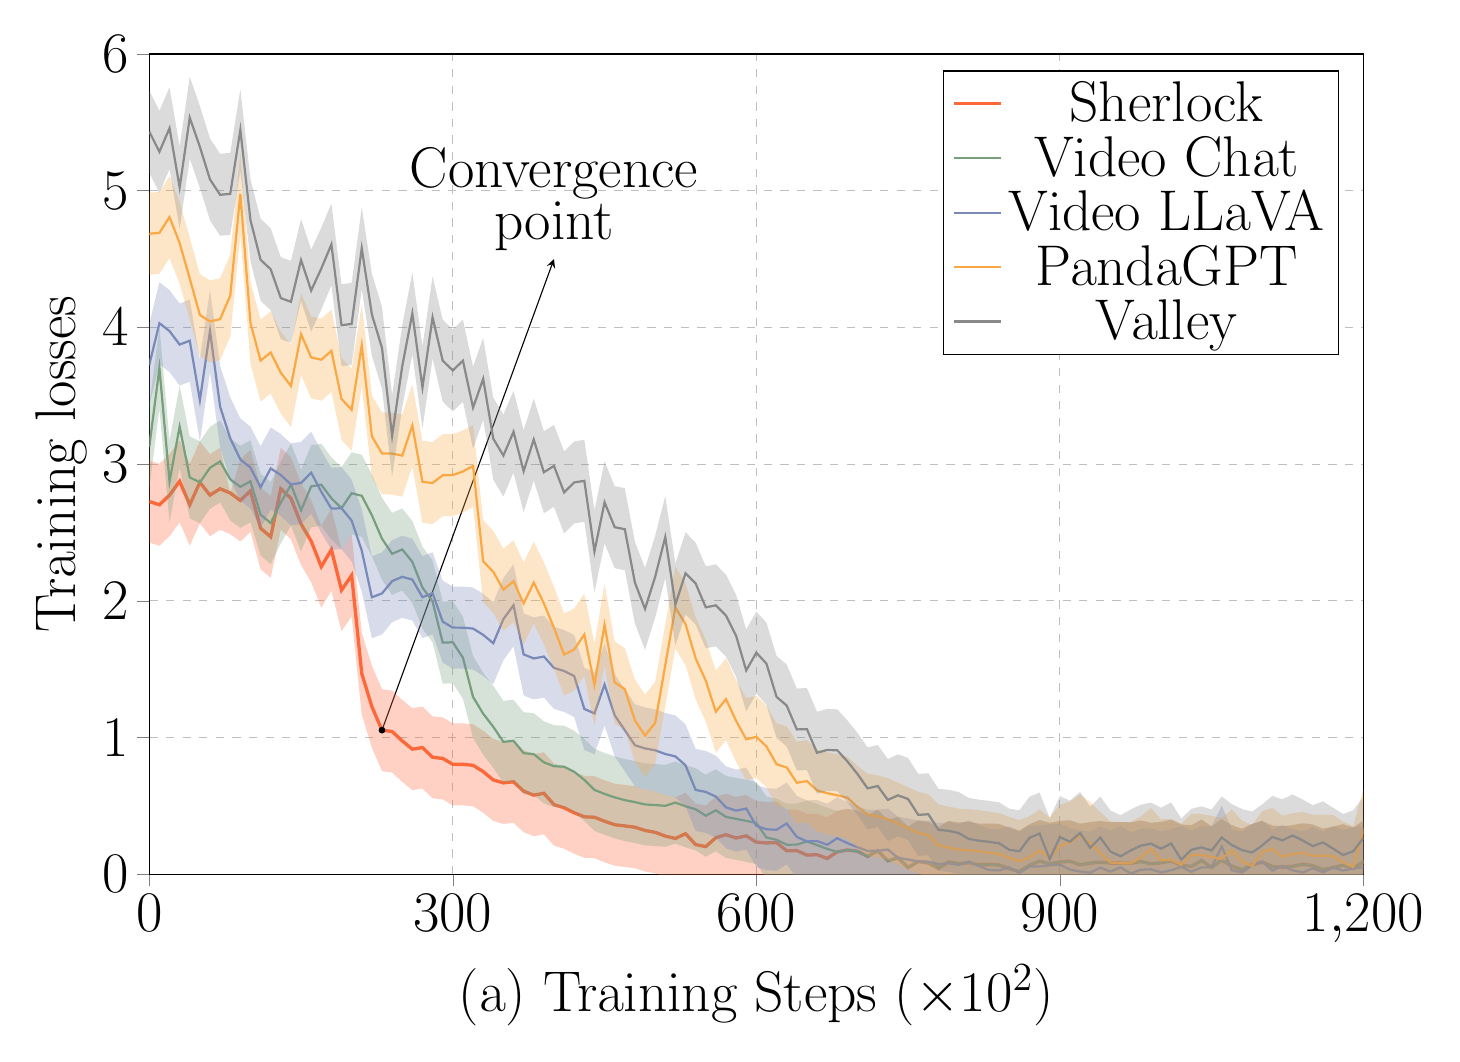
\begin{tikzpicture}
        \footnotesize
        \label{fig:train}
        \begin{axis}[
            xmin=0, xmax=1200, % x轴范围
            ymin=0, ymax=6, % y轴范围
            ytick={0, 1, 2, 3, 4, 5, 6},
            xtick={0, 300, 600, 900, 1200, 1500}, % x轴刻度
            xlabel={(a) Training Steps ($\times 10^2$)},
            xlabel style={font=\fontsize{22pt}{28pt}\selectfont},
            ylabel={Training losses},
            ylabel near ticks,
            ylabel style={font=\fontsize{22pt}{28pt}\selectfont},
            legend style={font=\fontsize{22pt}{28pt}\selectfont},
            xtick align=outside,
            ytick align=outside,
            tick label style={font=\fontsize{22pt}{28pt}\selectfont},
            ytick style={font=\fontsize{22pt}{28pt}\selectfont},
            enlargelimits=false,
            xtick pos=bottom,
            ytick pos=left,
            grid=both,
            grid style={dashed},
            width=17cm,
            height=12cm,
            xlabel style={at={(axis description cs:0.5,-0.1)},anchor=north}, % 手动调整xlabel位置
        ]
\addplot [only marks, mark=*, mark size=1pt, forget plot] coordinates {(230,1.0547)};
\draw[-stealth] (axis cs:230,1.0547) -- (axis cs:400,4.5) node[above, align=center] {\fontsize{22pt}{28pt}\selectfont Convergence \\ \fontsize{22pt}{28pt}\selectfont point};
\addplot [
            draw=none, % 不显示边界线
            fill=color3, % 设置阴影颜色
            fill opacity=0.3, % 设置透明度
            domain=0:60,
            samples=100,
            forget plot
        ]
        coordinates {%%add point
(0,3.0266)
(10,3.0031)
(20,3.0734)
(30,3.175)
(40,3.0031)
(50,3.1672)
(60,3.0734)
(70,3.1203)
(80,2.7891)
(90,3.0344)
(100,3.1047)
(110,2.8312)
(120,2.7688)
(130,3.1203)
(140,3.05)
(150,2.8625)
(160,2.7375)
(170,2.55)
(180,2.675)
(190,2.3781)
(200,2.4875)
(210,1.7688)
(220,1.5266)
(230,1.3547)
(240,1.3445)
(250,1.2762)
(260,1.2156)
(270,1.2273)
(280,1.156)
(290,1.148)
(300,1.1048)
(310,1.1043)
(320,1.0978)
(330,1.0516)
(340,0.9906)
(350,0.969)
(360,0.977)
(370,0.9086)
(380,0.8793)
(390,0.893)
(400,0.81)
(410,0.7874)
(420,0.75)
(430,0.721)
(440,0.7177)
(450,0.6883)
(460,0.6631)
(470,0.6543)
(480,0.6445)
(490,0.6211)
(500,0.6074)
(510,0.5801)
(520,0.5625)
(530,0.5977)
(540,0.5176)
(550,0.5029)
(560,0.5684)
(570,0.5902)
(580,0.5658)
(590,0.5814)
(600,0.5355)
(610,0.5297)
(620,0.5326)
(630,0.4721)
(640,0.474)
(650,0.4408)
(660,0.4438)
(670,0.4164)
(680,0.4642)
(690,0.4783)
(700,0.4686)
(710,0.4314)
(720,0.4725)
(730,0.3982)
(740,0.4212)
(750,0.35)
(760,0.3943)
(770,0.3831)
(780,0.3445)
(790,0.3909)
(800,0.3787)
(810,0.3848)
(820,0.3707)
(830,0.3714)
(840,0.3687)
(850,0.3411)
(860,0.3201)
(870,0.3665)
(880,0.3972)
(890,0.3769)
(900,0.3906)
(910,0.3952)
(920,0.3704)
(930,0.3823)
(940,0.3894)
(950,0.382)
(960,0.382)
(970,0.3806)
(980,0.3936)
(990,0.3771)
(1000,0.3837)
(1010,0.3994)
(1020,0.3647)
(1030,0.3587)
(1040,0.4011)
(1050,0.351)
(1060,0.4038)
(1070,0.3599)
(1080,0.3334)
(1090,0.3691)
(1100,0.3903)
(1110,0.3575)
(1120,0.3522)
(1130,0.3596)
(1140,0.3735)
(1150,0.3646)
(1160,0.3341)
(1170,0.3496)
(1180,0.3669)
(1190,0.343)
(1200,0.3925)
(1210,0.3385)
(1220,0.3446)
(1230,0.3404)
(1240,0.3582)
(1250,0.3248)
(1260,0.3498)
(1270,0.3406)
(1280,0.3496)
(1290,0.3615)
(1300,0.3456)
(1310,0.3415)
(1320,0.3366)
(1330,0.3453)
(1340,0.3696)
(1350,0.3464)
(1360,0.3492)
(1370,0.372)
(1380,0.352)
(1390,0.347)
(1400,0.3531)
(1410,0.3253)
(1420,0.3461)
(1430,0.3416)
(1440,0.3619)
(1450,0.3424)
(1460,0.3359)
(1470,0.3361)
(1480,0.3349)
(1490,0.3435)
(1500,0.3521)
(1500,0.0521-0.3)
(1490,0.0435-0.3)
(1480,0.0349-0.3)
(1470,0.0361-0.3)
(1460,0.0359-0.3)
(1450,0.0424-0.3)
(1440,0.0619-0.3)
(1430,0.0416-0.3)
(1420,0.0461-0.3)
(1410,0.0253-0.3)
(1400,0.0531-0.3)
(1390,0.047-0.3)
(1380,0.052-0.3)
(1370,0.072-0.3)
(1360,0.0492-0.3)
(1350,0.0464-0.3)
(1340,0.0696-0.3)
(1330,0.0453-0.3)
(1320,0.0366-0.3)
(1310,0.0415-0.3)
(1300,0.0456-0.3)
(1290,0.0615-0.3)
(1280,0.0496-0.3)
(1270,0.0406-0.3)
(1260,0.0498-0.3)
(1250,0.0248-0.3)
(1240,0.0582-0.3)
(1230,0.0404-0.3)
(1220,0.0446-0.3)
(1210,0.0385-0.3)
(1200,0.0925-0.3)
(1190,0.043-0.3)
(1180,0.0669-0.3)
(1170,0.0496-0.3)
(1160,0.0341-0.3)
(1150,0.0646-0.3)
(1140,0.0735-0.3)
(1130,0.0596-0.3)
(1120,0.0522-0.3)
(1110,0.0575-0.3)
(1100,0.0903-0.3)
(1090,0.0691-0.3)
(1080,0.0334-0.3)
(1070,0.0599-0.3)
(1060,0.1038-0.3)
(1050,0.051-0.3)
(1040,0.1011-0.3)
(1030,0.0587-0.3)
(1020,0.0647-0.3)
(1010,0.0994-0.3)
(1000,0.0837-0.3)
(990,0.0771-0.3)
(980,0.0936-0.3)
(970,0.0806-0.3)
(960,0.082-0.3)
(950,0.082-0.3)
(940,0.0894-0.3)
(930,0.0823-0.3)
(920,0.0704-0.3)
(910,0.0952-0.3)
(900,0.0906-0.3)
(890,0.0769-0.3)
(880,0.0972-0.3)
(870,0.0665-0.3)
(860,0.0201-0.3)
(850,0.0411-0.3)
(840,0.0687-0.3)
(830,0.0714-0.3)
(820,0.0707-0.3)
(810,0.0848-0.3)
(800,0.0787-0.3)
(790,0.0909-0.3)
(780,0.0445-0.3)
(770,0.0831-0.3)
(760,0.0943-0.3)
(750,0.05-0.3)
(740,0.1212-0.3)
(730,0.0982-0.3)
(720,0.1725-0.3)
(710,0.1314-0.3)
(700,0.1686-0.3)
(690,0.1783-0.3)
(680,0.1642-0.3)
(670,0.1164-0.3)
(660,0.1438-0.3)
(650,0.1408-0.3)
(640,0.174-0.3)
(630,0.1721-0.3)
(620,0.2326-0.3)
(610,0.2297-0.3)
(600,0.2355-0.3)
(590,0.2814-0.3)
(580,0.2658-0.3)
(570,0.2902-0.3)
(560,0.2684-0.3)
(550,0.2029-0.3)
(540,0.2176-0.3)
(530,0.2977-0.3)
(520,0.2625-0.3)
(510,0.2801-0.3)
(500,0.3074-0.3)
(490,0.3211-0.3)
(480,0.3445-0.3)
(470,0.3543-0.3)
(460,0.3631-0.3)
(450,0.3883-0.3)
(440,0.4177-0.3)
(430,0.421-0.3)
(420,0.45-0.3)
(410,0.4874-0.3)
(400,0.51-0.3)
(390,0.593-0.3)
(380,0.5793-0.3)
(370,0.6086-0.3)
(360,0.677-0.3)
(350,0.669-0.3)
(340,0.6906-0.3)
(330,0.7516-0.3)
(320,0.7978-0.3)
(310,0.8043-0.3)
(300,0.8048-0.3)
(290,0.848-0.3)
(280,0.856-0.3)
(270,0.9273-0.3)
(260,0.9156-0.3)
(250,0.9762-0.3)
(240,1.0445-0.3)
(230,1.0547-0.3)
(220,1.2266-0.3)
(210,1.4688-0.3)
(200,2.1875-0.3)
(190,2.0781-0.3)
(180,2.375-0.3)
(170,2.25-0.3)
(160,2.4375-0.3)
(150,2.5625-0.3)
(140,2.75-0.3)
(130,2.8203-0.3)
(120,2.4688-0.3)
(110,2.5312-0.3)
(100,2.8047-0.3)
(90,2.7344-0.3)
(80,2.7891-0.3)
(70,2.8203-0.3)
(60,2.7734-0.3)
(50,2.8672-0.3)
(40,2.7031-0.3)
(30,2.875-0.3)
(20,2.7734-0.3)
(10,2.7031-0.3)
(0,2.7266-0.3)


};-- cycle;


\addplot[color=color3,style={very thick}] coordinates{
(0,2.7266)
(10,2.7031)
(20,2.7734)
(30,2.875)
(40,2.7031)
(50,2.8672)
(60,2.7734)
(70,2.8203)
(80,2.7891)
(90,2.7344)
(100,2.8047)
(110,2.5312)
(120,2.4688)
(130,2.8203)
(140,2.75)
(150,2.5625)
(160,2.4375)
(170,2.25)
(180,2.375)
(190,2.0781)
(200,2.1875)
(210,1.4688)
(220,1.2266)
(230,1.0547)
(240,1.0445)
(250,0.9762)
(260,0.9156)
(270,0.9273)
(280,0.856)
(290,0.848)
(300,0.8048)
(310,0.8043)
(320,0.7978)
(330,0.7516)
(340,0.6906)
(350,0.669)
(360,0.677)
(370,0.6086)
(380,0.5793)
(390,0.593)
(400,0.51)
(410,0.4874)
(420,0.45)
(430,0.421)
(440,0.4177)
(450,0.3883)
(460,0.3631)
(470,0.3543)
(480,0.3445)
(490,0.3211)
(500,0.3074)
(510,0.2801)
(520,0.2625)
(530,0.2977)
(540,0.2176)
(550,0.2029)
(560,0.2684)
(570,0.2902)
(580,0.2658)
(590,0.2814)
(600,0.2355)
(610,0.2297)
(620,0.2326)
(630,0.1721)
(640,0.174)
(650,0.1408)
(660,0.1438)
(670,0.1164)
(680,0.1642)
(690,0.1783)
(700,0.1686)
(710,0.1314)
(720,0.1725)
(730,0.0982)
(740,0.1212)
(750,0.05)
(760,0.0943)
(770,0.0831)
(780,0.0445)
(790,0.0909)
(800,0.0787)
(810,0.0848)
(820,0.0707)
(830,0.0714)
(840,0.0687)
(850,0.0411)
(860,0.0201)
(870,0.0665)
(880,0.0972)
(890,0.0769)
(900,0.0906)
(910,0.0952)
(920,0.0704)
(930,0.0823)
(940,0.0894)
(950,0.082)
(960,0.082)
(970,0.0806)
(980,0.0936)
(990,0.0771)
(1000,0.0837)
(1010,0.0994)
(1020,0.0647)
(1030,0.0587)
(1040,0.1011)
(1050,0.051)
(1060,0.1038)
(1070,0.0599)
(1080,0.0334)
(1090,0.0691)
(1100,0.0903)
(1110,0.0575)
(1120,0.0522)
(1130,0.0596)
(1140,0.0735)
(1150,0.0646)
(1160,0.0341)
(1170,0.0496)
(1180,0.0669)
(1190,0.043)
(1200,0.0925)
(1210,0.0385)
(1220,0.0446)
(1230,0.0404)
(1240,0.0582)
(1250,0.0248)
(1260,0.0498)
(1270,0.0406)
(1280,0.0496)
(1290,0.0615)
(1300,0.0456)
(1310,0.0415)
(1320,0.0366)
(1330,0.0453)
(1340,0.0696)
(1350,0.0464)
(1360,0.0492)
(1370,0.072)
(1380,0.052)
(1390,0.047)
(1400,0.0531)
(1410,0.0253)
(1420,0.0461)
(1430,0.0416)
(1440,0.0619)
(1450,0.0424)
(1460,0.0359)
(1470,0.0361)
(1480,0.0349)
(1490,0.0435)
(1500,0.0521)};


\addplot [
            draw=none, % 不显示边界线
            fill=color1, % 设置阴影颜色
            fill opacity=0.3, % 设置透明度
            domain=0:60,
            samples=100,
            forget plot
        ]
        coordinates {%%videochat
        (0,3.1266 +0.3)
(10,3.7031 +0.3)
(20,2.8734 +0.3)
(30,3.275 +0.3)
(40,2.9031 +0.3)
(50,2.8672 +0.3)
(60,2.9734 +0.3)
(70,3.0203 +0.3)
(80,2.8891 +0.3)
(90,2.8344 +0.3)
(100,2.8747 +0.3)
(110,2.6312 +0.3)
(120,2.5688 +0.3)
(130,2.7203 +0.3)
(140,2.85 +0.3)
(150,2.6625 +0.3)
(160,2.8375 +0.3)
(170,2.85 +0.3)
(180,2.75 +0.3)
(190,2.6781 +0.3)
(200,2.7875 +0.3)
(210,2.7688 +0.3)
(220,2.6266 +0.3)
(230,2.4547 +0.3)
(240,2.3445 +0.3)
(250,2.3762 +0.3)
(260,2.2856 +0.3)
(270,2.0973 +0.3)
(280,1.9956 +0.3)
(290,1.6948 +0.3)
(300,1.69748 +0.3)
(310,1.58443 +0.3)
(320,1.2978 +0.3)
(330,1.17516 +0.3)
(340,1.07906 +0.3)
(350,0.969 +0.3)
(360,0.977 +0.3)
(370,0.886 +0.3)
(380,0.8793 +0.3)
(390,0.8193 +0.3)
(400,0.791 +0.3)
(410,0.7874 +0.3)
(420,0.75 +0.3)
(430,0.691 +0.3)
(440,0.6177 +0.3)
(450,0.5883 +0.3)
(460,0.5631 +0.3)
(470,0.543 +0.3)
(480,0.5285 +0.3)
(490,0.511 +0.3)
(500,0.5074 +0.3)
(510,0.501 +0.3)
(520,0.525 +0.3)
(530,0.4977 +0.3)
(540,0.476 +0.3)
(550,0.429 +0.3)
(560,0.4684 +0.3)
(570,0.4202 +0.3)
(580,0.4058 +0.3)
(590,0.3914 +0.3)
(600,0.3755 +0.3)
(610,0.2697 +0.3)
(620,0.2526 +0.3)
(630,0.21721 +0.3)
(640,0.2174 +0.3)
(650,0.2408 +0.3)
(660,0.2138 +0.3)
(670,0.1864 +0.3)
(680,0.1642 +0.3)
(690,0.1783 +0.3)
(700,0.1686 +0.3)
(710,0.1314 +0.3)
(720,0.1725 +0.3)
(730,0.0982 +0.3)
(740,0.1212 +0.3)
(750,0.05 +0.3)
(760,0.0943 +0.3)
(770,0.0831 +0.3)
(780,0.0445 +0.3)
(790,0.0909 +0.3)
(800,0.0787 +0.3)
(810,0.0848 +0.3)
(820,0.0707 +0.3)
(830,0.0714 +0.3)
(840,0.0687 +0.3)
(850,0.0411 +0.3)
(860,0.0201 +0.3)
(870,0.0665 +0.3)
(880,0.0972 +0.3)
(890,0.0769 +0.3)
(900,0.0906 +0.3)
(910,0.0952 +0.3)
(920,0.0704 +0.3)
(930,0.0823 +0.3)
(940,0.0894 +0.3)
(950,0.082 +0.3)
(960,0.082 +0.3)
(970,0.0806 +0.3)
(980,0.0936 +0.3)
(990,0.0771 +0.3)
(1000,0.0837 +0.3)
(1010,0.0994 +0.3)
(1020,0.0647 +0.3)
(1030,0.0587 +0.3)
(1040,0.1011 +0.3)
(1050,0.051 +0.3)
(1060,0.1038 +0.3)
(1070,0.0599 +0.3)
(1080,0.0334 +0.3)
(1090,0.0691 +0.3)
(1100,0.0903 +0.3)
(1110,0.0575 +0.3)
(1120,0.0522 +0.3)
(1130,0.0596 +0.3)
(1140,0.0735 +0.3)
(1150,0.0646 +0.3)
(1160,0.0341 +0.3)
(1170,0.0496 +0.3)
(1180,0.0669 +0.3)
(1190,0.043 +0.3)
(1200,0.0925 +0.3)
(1210,0.0385 +0.3)
(1220,0.0446 +0.3)
(1230,0.0404 +0.3)
(1240,0.0582 +0.3)
(1250,0.0248 +0.3)
(1260,0.0498 +0.3)
(1270,0.0406 +0.3)
(1280,0.0496 +0.3)
(1290,0.0615 +0.3)
(1300,0.0456 +0.3)
(1310,0.0415 +0.3)
(1320,0.0366 +0.3)
(1330,0.0453 +0.3)
(1340,0.0696 +0.3)
(1350,0.0464 +0.3)
(1360,0.0492 +0.3)
(1370,0.072 +0.3)
(1380,0.052 +0.3)
(1390,0.047 +0.3)
(1400,0.0531 +0.3)
(1410,0.0253 +0.3)
(1420,0.0461 +0.3)
(1430,0.0416 +0.3)
(1440,0.0619 +0.3)
(1450,0.0424 +0.3)
(1460,0.0359 +0.3)
(1470,0.0361 +0.3)
(1480,0.0349 +0.3)
(1490,0.0435 +0.3)
(1500,0.0521 +0.3)
(1500,0.0521 -0.3)
(1490,0.0435 -0.3)
(1480,0.0349 -0.3)
(1470,0.0361 -0.3)
(1460,0.0359 -0.3)
(1450,0.0424 -0.3)
(1440,0.0619 -0.3)
(1430,0.0416 -0.3)
(1420,0.0461 -0.3)
(1410,0.0253 -0.3)
(1400,0.0531 -0.3)
(1390,0.047 -0.3)
(1380,0.052 -0.3)
(1370,0.072 -0.3)
(1360,0.0492 -0.3)
(1350,0.0464 -0.3)
(1340,0.0696 -0.3)
(1330,0.0453 -0.3)
(1320,0.0366 -0.3)
(1310,0.0415 -0.3)
(1300,0.0456 -0.3)
(1290,0.0615 -0.3)
(1280,0.0496 -0.3)
(1270,0.0406 -0.3)
(1260,0.0498 -0.3)
(1250,0.0248 -0.3)
(1240,0.0582 -0.3)
(1230,0.0404 -0.3)
(1220,0.0446 -0.3)
(1210,0.0385 -0.3)
(1200,0.0925 -0.3)
(1190,0.043 -0.3)
(1180,0.0669 -0.3)
(1170,0.0496 -0.3)
(1160,0.0341 -0.3)
(1150,0.0646 -0.3)
(1140,0.0735 -0.3)
(1130,0.0596 -0.3)
(1120,0.0522 -0.3)
(1110,0.0575 -0.3)
(1100,0.0903 -0.3)
(1090,0.0691 -0.3)
(1080,0.0334 -0.3)
(1070,0.0599 -0.3)
(1060,0.1038 -0.3)
(1050,0.051 -0.3)
(1040,0.1011 -0.3)
(1030,0.0587 -0.3)
(1020,0.0647 -0.3)
(1010,0.0994 -0.3)
(1000,0.0837 -0.3)
(990,0.0771 -0.3)
(980,0.0936 -0.3)
(970,0.0806 -0.3)
(960,0.082 -0.3)
(950,0.082 -0.3)
(940,0.0894 -0.3)
(930,0.0823 -0.3)
(920,0.0704 -0.3)
(910,0.0952 -0.3)
(900,0.0906 -0.3)
(890,0.0769 -0.3)
(880,0.0972 -0.3)
(870,0.0665 -0.3)
(860,0.0201 -0.3)
(850,0.0411 -0.3)
(840,0.0687 -0.3)
(830,0.0714 -0.3)
(820,0.0707 -0.3)
(810,0.0848 -0.3)
(800,0.0787 -0.3)
(790,0.0909 -0.3)
(780,0.0445 -0.3)
(770,0.0831 -0.3)
(760,0.0943 -0.3)
(750,0.05 -0.3)
(740,0.1212 -0.3)
(730,0.0982 -0.3)
(720,0.1725 -0.3)
(710,0.1314 -0.3)
(700,0.1686 -0.3)
(690,0.1783 -0.3)
(680,0.1642 -0.3)
(670,0.1864 -0.3)
(660,0.2138 -0.3)
(650,0.2408 -0.3)
(640,0.2174 -0.3)
(630,0.21721 -0.3)
(620,0.2526 -0.3)
(610,0.2697 -0.3)
(600,0.3755 -0.3)
(590,0.3914 -0.3)
(580,0.4058 -0.3)
(570,0.4202 -0.3)
(560,0.4684 -0.3)
(550,0.429 -0.3)
(540,0.476 -0.3)
(530,0.4977 -0.3)
(520,0.525 -0.3)
(510,0.501 -0.3)
(500,0.5074 -0.3)
(490,0.511 -0.3)
(480,0.5285 -0.3)
(470,0.543 -0.3)
(460,0.5631 -0.3)
(450,0.5883 -0.3)
(440,0.6177 -0.3)
(430,0.691 -0.3)
(420,0.75 -0.3)
(410,0.7874 -0.3)
(400,0.791 -0.3)
(390,0.8193 -0.3)
(380,0.8793 -0.3)
(370,0.886 -0.3)
(360,0.977 -0.3)
(350,0.969 -0.3)
(340,1.07906 -0.3)
(330,1.17516 -0.3)
(320,1.2978 -0.3)
(310,1.58443 -0.3)
(300,1.69748 -0.3)
(290,1.6948 -0.3)
(280,1.9956 -0.3)
(270,2.0973 -0.3)
(260,2.2856 -0.3)
(250,2.3762 -0.3)
(240,2.3445 -0.3)
(230,2.4547 -0.3)
(220,2.6266 -0.3)
(210,2.7688 -0.3)
(200,2.7875 -0.3)
(190,2.6781 -0.3)
(180,2.75 -0.3)
(170,2.85 -0.3)
(160,2.8375 -0.3)
(150,2.6625 -0.3)
(140,2.85 -0.3)
(130,2.7203 -0.3)
(120,2.5688 -0.3)
(110,2.6312 -0.3)
(100,2.8747 -0.3)
(90,2.8344 -0.3)
(80,2.8891 -0.3)
(70,3.0203 -0.3)
(60,2.9734 -0.3)
(50,2.8672 -0.3)
(40,2.9031 -0.3)
(30,3.275 -0.3)
(20,2.8734 -0.3)
(10,3.7031 -0.3)
(0,3.1266 -0.3)
        };

\addplot[color=color1, style={thick}] coordinates{%%videochat
(0,3.1266)
(10,3.7031)
(20,2.8734)
(30,3.275)
(40,2.9031)
(50,2.8672)
(60,2.9734)
(70,3.0203)
(80,2.8891)
(90,2.8344)
(100,2.8747)
(110,2.6312)
(120,2.5688)
(130,2.7203)
(140,2.85)
(150,2.6625)
(160,2.8375)
(170,2.85)
(180,2.75)
(190,2.6781)
(200,2.7875)
(210,2.7688)
(220,2.6266)
(230,2.4547)
(240,2.3445)
(250,2.3762)
(260,2.2856)
(270,2.0973)
(280,1.9956)
(290,1.6948)
(300,1.69748)
(310,1.58443)
(320,1.2978)
(330,1.17516)
(340,1.07906)
(350,0.969)
(360,0.977)
(370,0.886)
(380,0.8793)
(390,0.8193)
(400,0.791)
(410,0.7874)
(420,0.75)
(430,0.691)
(440,0.6177)
(450,0.5883)
(460,0.5631)
(470,0.543)
(480,0.5285)
(490,0.511)
(500,0.5074)
(510,0.501)
(520,0.525)
(530,0.4977)
(540,0.476)
(550,0.429)
(560,0.4684)
(570,0.4202)
(580,0.4058)
(590,0.3914)
(600,0.3755)
(610,0.2697)
(620,0.2526)
(630,0.21721)
(640,0.2174)
(650,0.2408)
(660,0.2138)
(670,0.1864)
(680,0.1642)
(690,0.1783)
(700,0.1686)
(710,0.1314)
(720,0.1725)
(730,0.0982)
(740,0.1212)
(750,0.05)
(760,0.0943)
(770,0.0831)
(780,0.0445)
(790,0.0909)
(800,0.0787)
(810,0.0848)
(820,0.0707)
(830,0.0714)
(840,0.0687)
(850,0.0411)
(860,0.0201)
(870,0.0665)
(880,0.0972)
(890,0.0769)
(900,0.0906)
(910,0.0952)
(920,0.0704)
(930,0.0823)
(940,0.0894)
(950,0.082)
(960,0.082)
(970,0.0806)
(980,0.0936)
(990,0.0771)
(1000,0.0837)
(1010,0.0994)
(1020,0.0647)
(1030,0.0587)
(1040,0.1011)
(1050,0.051)
(1060,0.1038)
(1070,0.0599)
(1080,0.0334)
(1090,0.0691)
(1100,0.0903)
(1110,0.0575)
(1120,0.0522)
(1130,0.0596)
(1140,0.0735)
(1150,0.0646)
(1160,0.0341)
(1170,0.0496)
(1180,0.0669)
(1190,0.043)
(1200,0.0925)
(1210,0.0385)
(1220,0.0446)
(1230,0.0404)
(1240,0.0582)
(1250,0.0248)
(1260,0.0498)
(1270,0.0406)
(1280,0.0496)
(1290,0.0615)
(1300,0.0456)
(1310,0.0415)
(1320,0.0366)
(1330,0.0453)
(1340,0.0696)
(1350,0.0464)
(1360,0.0492)
(1370,0.072)
(1380,0.052)
(1390,0.047)
(1400,0.0531)
(1410,0.0253)
(1420,0.0461)
(1430,0.0416)
(1440,0.0619)
(1450,0.0424)
(1460,0.0359)
(1470,0.0361)
(1480,0.0349)
(1490,0.0435)
(1500,0.0521)
};


\addplot [
            draw=none, % 不显示边界线
            fill=color5, % 设置阴影颜色
            fill opacity=0.3, % 设置透明度
            domain=0:60,
            samples=100,
            forget plot
        ]
        coordinates {
(0,3.7266 +0.3)
(10,4.031 +0.3)
(20,3.9734 +0.3)
(30,3.875 +0.3)
(40,3.9031 +0.3)
(50,3.4672 +0.3)
(60,3.9734 +0.3)
(70,3.4203 +0.3)
(80,3.1891 +0.3)
(90,3.0344 +0.3)
(100,2.9747 +0.3)
(110,2.8312 +0.3)
(120,2.9688 +0.3)
(130,2.9203 +0.3)
(140,2.8521 +0.3)
(150,2.8625 +0.3)
(160,2.9375 +0.3)
(170,2.7982 +0.3)
(180,2.675 +0.3)
(190,2.6781 +0.3)
(200,2.5875 +0.3)
(210,2.3688 +0.3)
(220,2.0266 +0.3)
(230,2.0547 +0.3)
(240,2.1445 +0.3)
(250,2.1762 +0.3)
(260,2.156 +0.3)
(270,2.0273 +0.3)
(280,2.056 +0.3)
(290,1.848 +0.3)
(300,1.8048 +0.3)
(310,1.8043 +0.3)
(320,1.7978 +0.3)
(330,1.7516 +0.3)
(340,1.6906 +0.3)
(350,1.8669 +0.3)
(360,1.9677 +0.3)
(370,1.6086 +0.3)
(380,1.5793 +0.3)
(390,1.593 +0.3)
(400,1.51 +0.3)
(410,1.4874 +0.3)
(420,1.45 +0.3)
(430,1.21 +0.3)
(440,1.177 +0.3)
(450,1.3883 +0.3)
(460,1.1631 +0.3)
(470,1.0543 +0.3)
(480,0.9445 +0.3)
(490,0.9211 +0.3)
(500,0.9074 +0.3)
(510,0.8801 +0.3)
(520,0.8625 +0.3)
(530,0.7977 +0.3)
(540,0.6176 +0.3)
(550,0.6029 +0.3)
(560,0.5684 +0.3)
(570,0.4902 +0.3)
(580,0.4658 +0.3)
(590,0.4814 +0.3)
(600,0.355 +0.3)
(610,0.3297 +0.3)
(620,0.326 +0.3)
(630,0.3721 +0.3)
(640,0.274 +0.3)
(650,0.2408 +0.3)
(660,0.2438 +0.3)
(670,0.2164 +0.3)
(680,0.2642 +0.3)
(690,0.2283 +0.3)
(700,0.1986 +0.3)
(710,0.1714 +0.3)
(720,0.1725 +0.3)
(730,0.182 +0.3)
(740,0.1212 +0.3)
(750,0.1087 +0.3)
(760,0.0943 +0.3)
(770,0.0931 +0.3)
(780,0.0745 +0.3)
(790,0.0809 +0.3)
(800,0.0687 +0.3)
(810,0.0948 +0.3)
(820,0.0607 +0.3)
(830,0.0314 +0.3)
(840,0.0287 +0.3)
(850,0.0511 +0.3)
(860,0.0101 +0.3)
(870,0.0565 +0.3)
(880,0.0572 +0.3)
(890,0.0669 +0.3)
(900,0.0706 +0.3)
(910,0.0352 +0.3)
(920,0.0204 +0.3)
(930,0.0123 +0.3)
(940,0.0494 +0.3)
(950,0.02 +0.3)
(960,0.052 +0.3)
(970,0.006 +0.3)
(980,0.0336 +0.3)
(990,0.0371 +0.3)
(1000,0.0137 +0.3)
(1010,0.0294 +0.3)
(1020,0.0547 +0.3)
(1030,0.0187 +0.3)
(1040,0.0511 +0.3)
(1050,0.051 +0.3)
(1060,0.2038 +0.3)
(1070,0.0299 +0.3)
(1080,0.0134 +0.3)
(1090,0.06591 +0.3)
(1100,0.09313 +0.3)
(1110,0.0275 +0.3)
(1120,0.0622 +0.3)
(1130,0.0296 +0.3)
(1140,0.0135 +0.3)
(1150,0.0446 +0.3)
(1160,0.0141 +0.3)
(1170,0.0496 +0.3)
(1180,0.0269 +0.3)
(1190,0.043 +0.3)
(1200,0.0525 +0.3)
(1210,0.0285 +0.3)
(1220,0.0546 +0.3)
(1230,0.0104 +0.3)
(1240,0.0482 +0.3)
(1250,0.0148 +0.3)
(1260,0.0498 +0.3)
(1270,0.0106 +0.3)
(1280,0.0796 +0.3)
(1290,0.0215 +0.3)
(1300,0.0656 +0.3)
(1310,0.0215 +0.3)
(1320,0.0566 +0.3)
(1330,0.0153 +0.3)
(1340,0.0296 +0.3)
(1350,0.0564 +0.3)
(1360,0.0392 +0.3)
(1370,0.062 +0.3)
(1380,0.02 +0.3)
(1390,0.027 +0.3)
(1400,0.031 +0.3)
(1410,0.053 +0.3)
(1420,0.061 +0.3)
(1430,0.016 +0.3)
(1440,0.019 +0.3)
(1450,0.024 +0.3)
(1460,0.059 +0.3)
(1470,0.061 +0.3)
(1480,0.049 +0.3)
(1490,0.035 +0.3)
(1500,0.021 +0.3)
(1500,0.021 -0.3)
(1490,0.035 -0.3)
(1480,0.049 -0.3)
(1470,0.061 -0.3)
(1460,0.059 -0.3)
(1450,0.024 -0.3)
(1440,0.019 -0.3)
(1430,0.016 -0.3)
(1420,0.061 -0.3)
(1410,0.053 -0.3)
(1400,0.031 -0.3)
(1390,0.027 -0.3)
(1380,0.02 -0.3)
(1370,0.062 -0.3)
(1360,0.0392 -0.3)
(1350,0.0564 -0.3)
(1340,0.0296 -0.3)
(1330,0.0153 -0.3)
(1320,0.0566 -0.3)
(1310,0.0215 -0.3)
(1300,0.0656 -0.3)
(1290,0.0215 -0.3)
(1280,0.0796 -0.3)
(1270,0.0106 -0.3)
(1260,0.0498 -0.3)
(1250,0.0148 -0.3)
(1240,0.0482 -0.3)
(1230,0.0104 -0.3)
(1220,0.0546 -0.3)
(1210,0.0285 -0.3)
(1200,0.0525 -0.3)
(1190,0.043 -0.3)
(1180,0.0269 -0.3)
(1170,0.0496 -0.3)
(1160,0.0141 -0.3)
(1150,0.0446 -0.3)
(1140,0.0135 -0.3)
(1130,0.0296 -0.3)
(1120,0.0622 -0.3)
(1110,0.0275 -0.3)
(1100,0.09313 -0.3)
(1090,0.06591 -0.3)
(1080,0.0134 -0.3)
(1070,0.0299 -0.3)
(1060,0.2038 -0.3)
(1050,0.051 -0.3)
(1040,0.0511 -0.3)
(1030,0.0187 -0.3)
(1020,0.0547 -0.3)
(1010,0.0294 -0.3)
(1000,0.0137 -0.3)
(990,0.0371 -0.3)
(980,0.0336 -0.3)
(970,0.006 -0.3)
(960,0.052 -0.3)
(950,0.02 -0.3)
(940,0.0494 -0.3)
(930,0.0123 -0.3)
(920,0.0204 -0.3)
(910,0.0352 -0.3)
(900,0.0706 -0.3)
(890,0.0669 -0.3)
(880,0.0572 -0.3)
(870,0.0565 -0.3)
(860,0.0101 -0.3)
(850,0.0511 -0.3)
(840,0.0287 -0.3)
(830,0.0314 -0.3)
(820,0.0607 -0.3)
(810,0.0948 -0.3)
(800,0.0687 -0.3)
(790,0.0809 -0.3)
(780,0.0745 -0.3)
(770,0.0931 -0.3)
(760,0.0943 -0.3)
(750,0.1087 -0.3)
(740,0.1212 -0.3)
(730,0.182 -0.3)
(720,0.1725 -0.3)
(710,0.1714 -0.3)
(700,0.1986 -0.3)
(690,0.2283 -0.3)
(680,0.2642 -0.3)
(670,0.2164 -0.3)
(660,0.2438 -0.3)
(650,0.2408 -0.3)
(640,0.274 -0.3)
(630,0.3721 -0.3)
(620,0.326 -0.3)
(610,0.3297 -0.3)
(600,0.355 -0.3)
(590,0.4814 -0.3)
(580,0.4658 -0.3)
(570,0.4902 -0.3)
(560,0.5684 -0.3)
(550,0.6029 -0.3)
(540,0.6176 -0.3)
(530,0.7977 -0.3)
(520,0.8625 -0.3)
(510,0.8801 -0.3)
(500,0.9074 -0.3)
(490,0.9211 -0.3)
(480,0.9445 -0.3)
(470,1.0543 -0.3)
(460,1.1631 -0.3)
(450,1.3883 -0.3)
(440,1.177 -0.3)
(430,1.21 -0.3)
(420,1.45 -0.3)
(410,1.4874 -0.3)
(400,1.51 -0.3)
(390,1.593 -0.3)
(380,1.5793 -0.3)
(370,1.6086 -0.3)
(360,1.9677 -0.3)
(350,1.8669 -0.3)
(340,1.6906 -0.3)
(330,1.7516 -0.3)
(320,1.7978 -0.3)
(310,1.8043 -0.3)
(300,1.8048 -0.3)
(290,1.848 -0.3)
(280,2.056 -0.3)
(270,2.0273 -0.3)
(260,2.156 -0.3)
(250,2.1762 -0.3)
(240,2.1445 -0.3)
(230,2.0547 -0.3)
(220,2.0266 -0.3)
(210,2.3688 -0.3)
(200,2.5875 -0.3)
(190,2.6781 -0.3)
(180,2.675 -0.3)
(170,2.7982 -0.3)
(160,2.9375 -0.3)
(150,2.8625 -0.3)
(140,2.8521 -0.3)
(130,2.9203 -0.3)
(120,2.9688 -0.3)
(110,2.8312 -0.3)
(100,2.9747 -0.3)
(90,3.0344 -0.3)
(80,3.1891 -0.3)
(70,3.4203 -0.3)
(60,3.9734 -0.3)
(50,3.4672 -0.3)
(40,3.9031 -0.3)
(30,3.875 -0.3)
(20,3.9734 -0.3)
(10,4.031 -0.3)
(0,3.7266 -0.3)

};
\addplot[color=color5, style={thick}] coordinates{
(0,3.7266)
(10,4.031)
(20,3.9734)
(30,3.875)
(40,3.9031)
(50,3.4672)
(60,3.9734)
(70,3.4203)
(80,3.1891)
(90,3.0344)
(100,2.9747)
(110,2.8312)
(120,2.9688)
(130,2.9203)
(140,2.8521)
(150,2.8625)
(160,2.9375)
(170,2.7982)
(180,2.675)
(190,2.6781)
(200,2.5875)
(210,2.3688)
(220,2.0266)
(230,2.0547)
(240,2.1445)
(250,2.1762)
(260,2.156)
(270,2.0273)
(280,2.056)
(290,1.848)
(300,1.8048)
(310,1.8043)
(320,1.7978)
(330,1.7516)
(340,1.6906)
(350,1.8669)
(360,1.9677)
(370,1.6086)
(380,1.5793)
(390,1.593)
(400,1.51)
(410,1.4874)
(420,1.45)
(430,1.21)
(440,1.177)
(450,1.3883)
(460,1.1631)
(470,1.0543)
(480,0.9445)
(490,0.9211)
(500,0.9074)
(510,0.8801)
(520,0.8625)
(530,0.7977)
(540,0.6176)
(550,0.6029)
(560,0.5684)
(570,0.4902)
(580,0.4658)
(590,0.4814)
(600,0.355)
(610,0.3297)
(620,0.326)
(630,0.3721)
(640,0.274)
(650,0.2408)
(660,0.2438)
(670,0.2164)
(680,0.2642)
(690,0.2283)
(700,0.1986)
(710,0.1714)
(720,0.1725)
(730,0.182)
(740,0.1212)
(750,0.1087)
(760,0.0943)
(770,0.0931)
(780,0.0745)
(790,0.0809)
(800,0.0687)
(810,0.0948)
(820,0.0607)
(830,0.0314)
(840,0.0287)
(850,0.0511)
(860,0.0101)
(870,0.0565)
(880,0.0572)
(890,0.0669)
(900,0.0706)
(910,0.0352)
(920,0.0204)
(930,0.0123)
(940,0.0494)
(950,0.02)
(960,0.052)
(970,0.006)
(980,0.0336)
(990,0.0371)
(1000,0.0137)
(1010,0.0294)
(1020,0.0547)
(1030,0.0187)
(1040,0.0511)
(1050,0.051)
(1060,0.2038)
(1070,0.0299)
(1080,0.0134)
(1090,0.06591)
(1100,0.09313)
(1110,0.0275)
(1120,0.0622)
(1130,0.0296)
(1140,0.0135)
(1150,0.0446)
(1160,0.0141)
(1170,0.0496)
(1180,0.0269)
(1190,0.043)
(1200,0.0525)
(1210,0.0285)
(1220,0.0546)
(1230,0.0104)
(1240,0.0482)
(1250,0.0148)
(1260,0.0498)
(1270,0.0106)
(1280,0.0796)
(1290,0.0215)
(1300,0.0656)
(1310,0.0215)
(1320,0.0566)
(1330,0.0153)
(1340,0.0296)
(1350,0.0564)
(1360,0.0392)
(1370,0.062)
(1380,0.02)
(1390,0.027)
(1400,0.031)
(1410,0.053)
(1420,0.061)
(1430,0.016)
(1440,0.019)
(1450,0.024)
(1460,0.059)
(1470,0.061)
(1480,0.049)
(1490,0.035)
(1500,0.021)
};   

\addplot [
            draw=none, % 不显示边界线
            fill=color4, % 设置阴影颜色
            fill opacity=0.3, % 设置透明度
            domain=0:60,
            samples=100,
            forget plot
        ]
        coordinates {
(0, 4.685706638258415 + 0.3)
(10, 4.692096205350077 + 0.3)
(20, 4.806887535956572 + 0.3)
(30, 4.617212444058337 + 0.3)
(40, 4.357571263200387 + 0.3)
(50, 4.090845863783862 + 0.3)
(60, 4.044407398856213 + 0.3)
(70, 4.060295059062724 + 0.3)
(80, 4.233001451820559 + 0.3)
(90, 4.976046608373924 + 0.3)
(100, 4.032269489114867 + 0.3)
(110, 3.7579028655970687 + 0.3)
(120, 3.816609515634798 + 0.3)
(130, 3.669055470574325 + 0.3)
(140, 3.5717177317300457 + 0.3)
(150, 3.950621570177329 + 0.3)
(160, 3.7806636656256575 + 0.3)
(170, 3.7642921816078 + 0.3)
(180, 3.828803959716703 + 0.3)
(190, 3.4767801876943707 + 0.3)
(200, 3.3977231726830327 + 0.3)
(210, 3.8689909461648455 + 0.3)
(220, 3.2038383586943194 + 0.3)
(230, 3.0789088566698333 + 0.3)
(240, 3.077586361722899 + 0.3)
(250, 3.0627166118828672 + 0.3)
(260, 3.2831343630045036 + 0.3)
(270, 2.870551361837176 + 0.3)
(280, 2.8622278212014506 + 0.3)
(290, 2.9190549925229525 + 0.3)
(300, 2.9202303620810588 + 0.3)
(310, 2.946752488092862 + 0.3)
(320, 2.986272173916546 + 0.3)
(330, 2.2901388041322445 + 0.3)
(340, 2.211914629180183 + 0.3)
(350, 2.082027614351317 + 0.3)
(360, 2.1440615952811495 + 0.3)
(370, 1.981565890090654 + 0.3)
(380, 2.133571955119862 + 0.3)
(390, 1.9824961706656548 + 0.3)
(400, 1.8029897611273425 + 0.3)
(410, 1.6075135456404203 + 0.3)
(420, 1.6444611962143419 + 0.3)
(430, 1.7540048682210557 + 0.3)
(440, 1.387103679408249 + 0.3)
(450, 1.824859054005592 + 0.3)
(460, 1.404092671709165 + 0.3)
(470, 1.3545068592516285 + 0.3)
(480, 1.1263697906783297 + 0.3)
(490, 1.0146120187397562 + 0.3)
(500, 1.1081285380888426 + 0.3)
(510, 1.5293361470688109 + 0.3)
(520, 1.9513019726854797 + 0.3)
(530, 1.8306404001431 + 0.3)
(540, 1.5805455490025538 + 0.3)
(550, 1.4168771596829192 + 0.3)
(560, 1.1893144725576 + 0.3)
(570, 1.281611314643375 + 0.3)
(580, 1.1224753171672489 + 0.3)
(590, 0.9877987374155352 + 0.3)
(600, 1.0054923489247605 + 0.3)
(610, 0.9353996445932457 + 0.3)
(620, 0.80505844253307486 + 0.3)
(630, 0.7816997716335113 + 0.3)
(640, 0.670085510728674 + 0.3)
(650, 0.6820227434957141 + 0.3)
(660, 0.614224892421447 + 0.3)
(670, 0.59334893069459693 + 0.3)
(680, 0.57815905940517067 + 0.3)
(690, 0.5607392791873497 + 0.3)
(700, 0.4925862544032219 + 0.3)
(710, 0.4363191520005 + 0.3)
(720, 0.42449712681651193 + 0.3)
(730, 0.4040100283122 + 0.3)
(740, 0.370307255024 + 0.3)
(750, 0.33743557731276 + 0.3)
(760, 0.30408080612587895 + 0.3)
(770, 0.285964311418387 + 0.3)
(780, 0.2116657581272811 + 0.3)
(790, 0.19625890084829925 + 0.3)
(800, 0.17999215301234342 + 0.3)
(810, 0.1753083921197 + 0.3)
(820, 0.170832629208 + 0.3)
(830, 0.157851165058704 + 0.3)
(840, 0.148616406733853964 + 0.3)
(850, 0.12045233381123697 + 0.3)
(860, 0.0964232347998881 + 0.3)
(870, 0.1253039405712316 + 0.3)
(880, 0.1750934188780679 + 0.3)
(890, 0.1150474489404642 + 0.3)
(900, 0.2082746574709541 + 0.3)
(910, 0.2326163042580064 + 0.3)
(920, 0.28455602848522185 + 0.3)
(930, 0.22908701317394324 + 0.3)
(940, 0.1555939354375399 + 0.3)
(950, 0.08618362034403205 + 0.3)
(960, 0.08197475283939822 + 0.3)
(970, 0.08086876742000367 + 0.3)
(980, 0.1235631700111424 + 0.3)
(990, 0.18585951630894615 + 0.3)
(1000, 0.10233688951268554 + 0.3)
(1010, 0.10723861755256653 + 0.3)
(1020, 0.06975706124877737 + 0.3)
(1030, 0.14329601824169475 + 0.3)
(1040, 0.1412384341200312 + 0.3)
(1050, 0.1268275735370564 + 0.3)
(1060, 0.11328943194651643 + 0.3)
(1070, 0.17511748548926733 + 0.3)
(1080, 0.0937073447317179 + 0.3)
(1090, 0.06133983428100904 + 0.3)
(1100, 0.1616254291204875 + 0.3)
(1110, 0.186631131496792 + 0.3)
(1120, 0.12957648826995282 + 0.3)
(1130, 0.1475829355139097 + 0.3)
(1140, 0.15711565173996666 + 0.3)
(1150, 0.13537800790177816 + 0.3)
(1160, 0.1372758645505045 + 0.3)
(1170, 0.1334572171892757 + 0.3)
(1180, 0.08752787469740634 + 0.3)
(1190, 0.054161890439325025 + 0.3)
(1200, 0.32434932519044395 + 0.3)
(1210, 0.25830393775757167 + 0.3)
(1220, 0.1136003942735258 + 0.3)
(1230, 0.1152705864773337 + 0.3)
(1240, 0.13841324485759566 + 0.3)
(1250, 0.13707584697875644 + 0.3)
(1260, 0.1605779444651323 + 0.3)
(1270, 0.1152400167665078 + 0.3)
(1280, 0.07130869919428225 + 0.3)
(1290, 0.2548904357872269 + 0.3)
(1300, 0.2790664761465989 + 0.3)
(1310, 0.24838746440586615 + 0.3)
(1320, 0.1598649966542332 + 0.3)
(1330, 0.14194518177984123 + 0.3)
(1340, 0.1163622010616498 + 0.3)
(1350, 0.2781206489359677 + 0.3)
(1360, 0.08915208331142557 + 0.3)
(1370, 0.2654466188398887 + 0.3)
(1380, 0.2632130855621416 + 0.3)
(1390, 0.23247727217597663 + 0.3)
(1400, 0.09735367664725594 + 0.3)
(1410, 0.1182584851293488 + 0.3)
(1420, 0.1438629735812925 + 0.3)
(1430, 0.1569632107005781 + 0.3)
(1440, 0.1829857568525291 + 0.3)
(1450, 0.1540328768706864 + 0.3)
(1460, 0.1355066252804602 + 0.3)
(1470, 0.04945774614073415 + 0.3)
(1480, 0.10507873232635291 + 0.3)
(1490, 0.11582634525513344 + 0.3)
(1500, 0.0138138567207493 + 0.3)
(1500, 0.0138138567207493 - 0.3)
(1490, 0.11582634525513344 - 0.3)
(1480, 0.10507873232635291 - 0.3)
(1470, 0.04945774614073415 - 0.3)
(1460, 0.1355066252804602 - 0.3)
(1450, 0.1540328768706864 - 0.3)
(1440, 0.1829857568525291 - 0.3)
(1430, 0.1569632107005781 - 0.3)
(1420, 0.1438629735812925 - 0.3)
(1410, 0.1182584851293488 - 0.3)
(1400, 0.09735367664725594 - 0.3)
(1390, 0.23247727217597663 - 0.3)
(1380, 0.2632130855621416 - 0.3)
(1370, 0.2654466188398887 - 0.3)
(1360, 0.08915208331142557 - 0.3)
(1350, 0.2781206489359677 - 0.3)
(1340, 0.1163622010616498 - 0.3)
(1330, 0.14194518177984123 - 0.3)
(1320, 0.1598649966542332 - 0.3)
(1310, 0.24838746440586615 - 0.3)
(1300, 0.2790664761465989 - 0.3)
(1290, 0.2548904357872269 - 0.3)
(1280, 0.07130869919428225 - 0.3)
(1270, 0.1152400167665078 - 0.3)
(1260, 0.1605779444651323 - 0.3)
(1250, 0.13707584697875644 - 0.3)
(1240, 0.13841324485759566 - 0.3)
(1230, 0.1152705864773337 - 0.3)
(1220, 0.1136003942735258 - 0.3)
(1210, 0.25830393775757167 - 0.3)
(1200, 0.32434932519044395 - 0.3)
(1190, 0.054161890439325025 - 0.3)
(1180, 0.08752787469740634 - 0.3)
(1170, 0.1334572171892757 - 0.3)
(1160, 0.1372758645505045 - 0.3)
(1150, 0.13537800790177816 - 0.3)
(1140, 0.15711565173996666 - 0.3)
(1130, 0.1475829355139097 - 0.3)
(1120, 0.12957648826995282 - 0.3)
(1110, 0.186631131496792 - 0.3)
(1100, 0.1616254291204875 - 0.3)
(1090, 0.06133983428100904 - 0.3)
(1080, 0.0937073447317179 - 0.3)
(1070, 0.17511748548926733 - 0.3)
(1060, 0.11328943194651643 - 0.3)
(1050, 0.1268275735370564 - 0.3)
(1040, 0.1412384341200312 - 0.3)
(1030, 0.14329601824169475 - 0.3)
(1020, 0.06975706124877737 - 0.3)
(1010, 0.10723861755256653 - 0.3)
(1000, 0.10233688951268554 - 0.3)
(990, 0.18585951630894615 - 0.3)
(980, 0.1235631700111424 - 0.3)
(970, 0.08086876742000367 - 0.3)
(960, 0.08197475283939822 - 0.3)
(950, 0.08618362034403205 - 0.3)
(940, 0.1555939354375399 - 0.3)
(930, 0.22908701317394324 - 0.3)
(920, 0.28455602848522185 - 0.3)
(910, 0.2326163042580064 - 0.3)
(900, 0.2082746574709541 - 0.3)
(890, 0.1150474489404642 - 0.3)
(880, 0.1750934188780679 - 0.3)
(870, 0.1253039405712316 - 0.3)
(860, 0.0964232347998881 - 0.3)
(850, 0.12045233381123697 - 0.3)
(840, 0.148616406733853964 - 0.3)
(830, 0.157851165058704 - 0.3)
(820, 0.170832629208 - 0.3)
(810, 0.1753083921197 - 0.3)
(800, 0.17999215301234342 - 0.3)
(790, 0.19625890084829925 - 0.3)
(780, 0.2116657581272811 - 0.3)
(770, 0.285964311418387 - 0.3)
(760, 0.30408080612587895 - 0.3)
(750, 0.33743557731276 - 0.3)
(740, 0.370307255024 - 0.3)
(730, 0.4040100283122 - 0.3)
(720, 0.42449712681651193 - 0.3)
(710, 0.4363191520005 - 0.3)
(700, 0.4925862544032219 - 0.3)
(690, 0.5607392791873497 - 0.3)
(680, 0.57815905940517067 - 0.3)
(670, 0.59334893069459693 - 0.3)
(660, 0.614224892421447 - 0.3)
(650, 0.6820227434957141 - 0.3)
(640, 0.670085510728674 - 0.3)
(630, 0.7816997716335113 - 0.3)
(620, 0.80505844253307486 - 0.3)
(610, 0.9353996445932457 - 0.3)
(600, 1.0054923489247605 - 0.3)
(590, 0.9877987374155352 - 0.3)
(580, 1.1224753171672489 - 0.3)
(570, 1.281611314643375 - 0.3)
(560, 1.1893144725576 - 0.3)
(550, 1.4168771596829192 - 0.3)
(540, 1.5805455490025538 - 0.3)
(530, 1.8306404001431 - 0.3)
(520, 1.9513019726854797 - 0.3)
(510, 1.5293361470688109 - 0.3)
(500, 1.1081285380888426 - 0.3)
(490, 1.0146120187397562 - 0.3)
(480, 1.1263697906783297 - 0.3)
(470, 1.3545068592516285 - 0.3)
(460, 1.404092671709165 - 0.3)
(450, 1.824859054005592 - 0.3)
(440, 1.387103679408249 - 0.3)
(430, 1.7540048682210557 - 0.3)
(420, 1.6444611962143419 - 0.3)
(410, 1.6075135456404203 - 0.3)
(400, 1.8029897611273425 - 0.3)
(390, 1.9824961706656548 - 0.3)
(380, 2.133571955119862 - 0.3)
(370, 1.981565890090654 - 0.3)
(360, 2.1440615952811495 - 0.3)
(350, 2.082027614351317 - 0.3)
(340, 2.211914629180183 - 0.3)
(330, 2.2901388041322445 - 0.3)
(320, 2.986272173916546 - 0.3)
(310, 2.946752488092862 - 0.3)
(300, 2.9202303620810588 - 0.3)
(290, 2.9190549925229525 - 0.3)
(280, 2.8622278212014506 - 0.3)
(270, 2.870551361837176 - 0.3)
(260, 3.2831343630045036 - 0.3)
(250, 3.0627166118828672 - 0.3)
(240, 3.077586361722899 - 0.3)
(230, 3.0789088566698333 - 0.3)
(220, 3.2038383586943194 - 0.3)
(210, 3.8689909461648455 - 0.3)
(200, 3.3977231726830327 - 0.3)
(190, 3.4767801876943707 - 0.3)
(180, 3.828803959716703 - 0.3)
(170, 3.7642921816078 - 0.3)
(160, 3.7806636656256575 - 0.3)
(150, 3.950621570177329 - 0.3)
(140, 3.5717177317300457 - 0.3)
(130, 3.669055470574325 - 0.3)
(120, 3.816609515634798 - 0.3)
(110, 3.7579028655970687 - 0.3)
(100, 4.032269489114867 - 0.3)
(90, 4.976046608373924 - 0.3)
(80, 4.233001451820559 - 0.3)
(70, 4.060295059062724 - 0.3)
(60, 4.044407398856213 - 0.3)
(50, 4.090845863783862 - 0.3)
(40, 4.357571263200387 - 0.3)
(30, 4.617212444058337 - 0.3)
(20, 4.806887535956572 - 0.3)
(10, 4.692096205350077 - 0.3)
(0, 4.685706638258415 - 0.3)
};
\addplot[color=color4, style={thick}] coordinates{
(0, 4.685706638258415)
(10, 4.692096205350077)
(20, 4.806887535956572)
(30, 4.617212444058337)
(40, 4.357571263200387)
(50, 4.090845863783862)
(60, 4.044407398856213)
(70, 4.060295059062724)
(80, 4.233001451820559)
(90, 4.976046608373924)
(100, 4.032269489114867)
(110, 3.7579028655970687)
(120, 3.816609515634798)
(130, 3.669055470574325)
(140, 3.5717177317300457)
(150, 3.950621570177329)
(160, 3.7806636656256575)
(170, 3.7642921816078)
(180, 3.828803959716703)
(190, 3.4767801876943707)
(200, 3.3977231726830327)
(210, 3.8689909461648455)
(220, 3.2038383586943194)
(230, 3.0789088566698333)
(240, 3.077586361722899)
(250, 3.0627166118828672)
(260, 3.2831343630045036)
(270, 2.870551361837176)
(280, 2.8622278212014506)
(290, 2.9190549925229525)
(300, 2.9202303620810588)
(310, 2.946752488092862)
(320, 2.986272173916546)
(330, 2.2901388041322445)
(340, 2.211914629180183)
(350, 2.082027614351317)
(360, 2.1440615952811495)
(370, 1.981565890090654)
(380, 2.133571955119862)
(390, 1.9824961706656548)
(400, 1.8029897611273425)
(410, 1.6075135456404203)
(420, 1.6444611962143419)
(430, 1.7540048682210557)
(440, 1.387103679408249)
(450, 1.824859054005592)
(460, 1.404092671709165)
(470, 1.3545068592516285)
(480, 1.1263697906783297)
(490, 1.0146120187397562)
(500, 1.1081285380888426)
(510, 1.5293361470688109)
(520, 1.9513019726854797)
(530, 1.8306404001431)
(540, 1.5805455490025538)
(550, 1.4168771596829192)
(560, 1.1893144725576)
(570, 1.281611314643375)
(580, 1.1224753171672489)
(590, 0.9877987374155352)
(600, 1.0054923489247605)
(610, 0.9353996445932457)
(620, 0.80505844253307486)
(630, 0.7816997716335113)
(640, 0.670085510728674)
(650, 0.6820227434957141)
(660, 0.614224892421447)
(670, 0.59334893069459693)
(680, 0.57815905940517067)
(690, 0.5607392791873497)
(700, 0.4925862544032219)
(710, 0.4363191520005)
(720, 0.42449712681651193)
(730, 0.4040100283122)
(740, 0.370307255024)
(750, 0.33743557731276)
(760, 0.30408080612587895)
(770, 0.285964311418387)
(780, 0.2116657581272811)
(790, 0.19625890084829925)
(800, 0.17999215301234342)
(810, 0.1753083921197)
(820, 0.170832629208)
(830, 0.157851165058704)
(840, 0.148616406733853964)
(850, 0.12045233381123697)
(860, 0.0964232347998881)
(870, 0.1253039405712316)
(880, 0.1750934188780679)
(890, 0.1150474489404642)
(900, 0.2082746574709541)
(910, 0.2326163042580064)
(920, 0.28455602848522185)
(930, 0.22908701317394324)
(940, 0.1555939354375399)
(950, 0.08618362034403205)
(960, 0.08197475283939822)
(970, 0.08086876742000367)
(980, 0.1235631700111424)
(990, 0.18585951630894615)
(1000, 0.10233688951268554)
(1010, 0.10723861755256653)
(1020, 0.06975706124877737)
(1030, 0.14329601824169475)
(1040, 0.1412384341200312)
(1050, 0.1268275735370564)
(1060, 0.11328943194651643)
(1070, 0.17511748548926733)
(1080, 0.0937073447317179)
(1090, 0.06133983428100904)
(1100, 0.1616254291204875)
(1110, 0.186631131496792)
(1120, 0.12957648826995282)
(1130, 0.1475829355139097)
(1140, 0.15711565173996666)
(1150, 0.13537800790177816)
(1160, 0.1372758645505045)
(1170, 0.1334572171892757)
(1180, 0.08752787469740634)
(1190, 0.054161890439325025)
(1200, 0.32434932519044395)
(1210, 0.25830393775757167)
(1220, 0.1136003942735258)
(1230, 0.1152705864773337)
(1240, 0.13841324485759566)
(1250, 0.13707584697875644)
(1260, 0.1605779444651323)
(1270, 0.1152400167665078)
(1280, 0.07130869919428225)
(1290, 0.2548904357872269)
(1300, 0.2790664761465989)
(1310, 0.24838746440586615)
(1320, 0.1598649966542332)
(1330, 0.14194518177984123)
(1340, 0.1163622010616498)
(1350, 0.2781206489359677)
(1360, 0.08915208331142557)
(1370, 0.2654466188398887)
(1380, 0.2632130855621416)
(1390, 0.23247727217597663)
(1400, 0.09735367664725594)
(1410, 0.1182584851293488)
(1420, 0.1438629735812925)
(1430, 0.1569632107005781)
(1440, 0.1829857568525291)
(1450, 0.1540328768706864)
(1460, 0.1355066252804602)
(1470, 0.04945774614073415)
(1480, 0.10507873232635291)
(1490, 0.11582634525513344)
(1500, 0.0138138567207493)
};

\addplot [
            draw=none, % 不显示边界线
            fill=color8, % 设置阴影颜色
            fill opacity=0.3, % 设置透明度
            domain=0:60,
            samples=100,
            forget plot
        ]
        coordinates {(0, 5.432333692324405 + 0.3)
(10, 5.284783671858206 + 0.3)
(20, 5.457359148084505 + 0.3)
(30, 5.023533452254388 + 0.3)
(40, 5.534376264948586 + 0.3)
(50, 5.320741036199024 + 0.3)
(60, 5.082680237341437 + 0.3)
(70, 4.970221285492551 + 0.3)
(80, 4.976975068555395 + 0.3)
(90, 5.445019526332374 + 0.3)
(100, 4.785254926007498 + 0.3)
(110, 4.494933944133198 + 0.3)
(120, 4.425496991951899 + 0.3)
(130, 4.214698591843256 + 0.3)
(140, 4.187293292655978 + 0.3)
(150, 4.493215617250431 + 0.3)
(160, 4.269907125677115 + 0.3)
(170, 4.430670320145285 + 0.3)
(180, 4.607805450821287 + 0.3)
(190, 4.016659523767325 + 0.3)
(200, 4.025768048820833 + 0.3)
(210, 4.57893515908593 + 0.3)
(220, 4.094643107277234 + 0.3)
(230, 3.850185337376338 + 0.3)
(240, 3.207176741896641 + 0.3)
(250, 3.715817353624102 + 0.3)
(260, 4.102483178734463 + 0.3)
(270, 3.560953980836053 + 0.3)
(280, 4.073194867304199 + 0.3)
(290, 3.757177609323955 + 0.3)
(300, 3.685677370470023 + 0.3)
(310, 3.757026874034428 + 0.3)
(320, 3.413397230234476 + 0.3)
(330, 3.623636404219252 + 0.3)
(340, 3.186421658224503 + 0.3)
(350, 3.062798248384900 + 0.3)
(360, 3.237049960813956 + 0.3)
(370, 2.949030759304928 + 0.3)
(380, 3.180295899825470 + 0.3)
(390, 2.941051540812777 + 0.3)
(400, 2.987219839772595 + 0.3)
(410, 2.793527395343425 + 0.3)
(420, 2.8668258052027703 + 0.3)
(430, 2.8781037151509837 + 0.3)
(440, 2.3620780149581665 + 0.3)
(450, 2.721138228256038 + 0.3)
(460, 2.5393581720100787 + 0.3)
(470, 2.524253722005256 + 0.3)
(480, 2.1335928655505485 + 0.3)
(490, 1.9414388268464671 + 0.3)
(500, 2.1763640597046086 + 0.3)
(510, 2.4666727179724096 + 0.3)
(520, 1.9731139711342068 + 0.3)
(530, 2.2021086129262876 + 0.3)
(540, 2.1279516230315246 + 0.3)
(550, 1.9531511267818211 + 0.3)
(560, 1.9675482288423172 + 0.3)
(570, 1.8928411569888196 + 0.3)
(580, 1.7451039212852656 + 0.3)
(590, 1.4912581078460274 + 0.3)
(600, 1.6211385499244975 + 0.3)
(610, 1.5410469490169425 + 0.3)
(620, 1.2978278808022452 + 0.3)
(630, 1.2348347586636559 + 0.3)
(640, 1.0600402781617072 + 0.3)
(650, 1.0624117661835597 + 0.3)
(660, 0.8891444039251843 + 0.3)
(670, 0.9098677092796561 + 0.3)
(680, 0.9070854843500436 + 0.3)
(690, 0.8264951032161687 + 0.3)
(700, 0.7336797740283408 + 0.3)
(710, 0.6289699562923862 + 0.3)
(720, 0.6462642380052526 + 0.3)
(730, 0.544375691787224 + 0.3)
(740, 0.5777879300918026 + 0.3)
(750, 0.5511977135498523 + 0.3)
(760, 0.4350983845001655 + 0.3)
(770, 0.4397588804736735 + 0.3)
(780, 0.3257552829608907 + 0.3)
(790, 0.31834506799345013 + 0.3)
(800, 0.3023715481700019 + 0.3)
(810, 0.2591115808578816 + 0.3)
(820, 0.24630979854621315 + 0.3)
(830, 0.23773908997559465 + 0.3)
(840, 0.22656872856190344 + 0.3)
(850, 0.17973043056527684 + 0.3)
(860, 0.16860959885786616 + 0.3)
(870, 0.2676768995401792 + 0.3)
(880, 0.2982259349652473 + 0.3)
(890, 0.1111168950330856 + 0.3)
(900, 0.2721022852946586 + 0.3)
(910, 0.23893191557272637 + 0.3)
(920, 0.3025494025900251 + 0.3)
(930, 0.19451026210115424 + 0.3)
(940, 0.2696385812309028 + 0.3)
(950, 0.16664275171121782 + 0.3)
(960, 0.13207493158171372 + 0.3)
(970, 0.17492660710587286 + 0.3)
(980, 0.2094467022499813 + 0.3)
(990, 0.22441188299676934 + 0.3)
(1000, 0.18769172873639379 + 0.3)
(1010, 0.22574313750468689 + 0.3)
(1020, 0.10784535025867275 + 0.3)
(1030, 0.17980615116174385 + 0.3)
(1040, 0.19725787228610753 + 0.3)
(1050, 0.17423547594746759 + 0.3)
(1060, 0.2697234111292698 + 0.3)
(1070, 0.2138766220485051 + 0.3)
(1080, 0.17735148158076147 + 0.3)
(1090, 0.15947357945313942 + 0.3)
(1100, 0.21164836863031537 + 0.3)
(1110, 0.2737115815116754 + 0.3)
(1120, 0.24875839961920996 + 0.3)
(1130, 0.284178558144909 + 0.3)
(1140, 0.2472307522527075 + 0.3)
(1150, 0.20697224875448568 + 0.3)
(1160, 0.23341857249236582 + 0.3)
(1170, 0.1882408655575173 + 0.3)
(1180, 0.1416773914042334 + 0.3)
(1190, 0.16918754022855625 + 0.3)
(1200, 0.2658054306020206 + 0.3)
(1210, 0.26143638367063066 + 0.3)
(1220, 0.12326144025456514 + 0.3)
(1230, 0.1651500876148937 + 0.3)
(1240, 0.11038596890627402 + 0.3)
(1250, 0.15566052456948952 + 0.3)
(1260, 0.2693589495026258 + 0.3)
(1270, 0.09959131711892034 + 0.3)
(1280, 0.0886414497170574 + 0.3)
(1290, 0.2629296769133326 + 0.3)
(1300, 0.2622500861557261 + 0.3)
(1310, 0.21955136948245551 + 0.3)
(1320, 0.19121657776195236 + 0.3)
(1330, 0.1529053148774103 + 0.3)
(1340, 0.21254213250463962 + 0.3)
(1350, 0.2516236269022696 + 0.3)
(1360, 0.1402344738092955 + 0.3)
(1370, 0.1973506900292578 + 0.3)
(1380, 0.2611537872955854 + 0.3)
(1390, 0.17651444068636275 + 0.3)
(1400, 0.11436274155805536 + 0.3)
(1410, 0.14596906610520982 + 0.3)
(1420, 0.1760719423369747 + 0.3)
(1430, 0.19572089169221293 + 0.3)
(1440, 0.2259203145488826 + 0.3)
(1450, 0.1650677314988124 + 0.3)
(1460, 0.15232251963644733 + 0.3)
(1470, 0.07092582737772411 + 0.3)
(1480, 0.1374376943861968 + 0.3)
(1490, 0.13320740926837655 + 0.3)
(1500, 0.09679864081978637 + 0.3)
(1500, 0.09679864081978637 - 0.3)
(1490, 0.13320740926837655 - 0.3)
(1480, 0.1374376943861968 - 0.3)
(1470, 0.07092582737772411 - 0.3)
(1460, 0.15232251963644733 - 0.3)
(1450, 0.1650677314988124 - 0.3)
(1440, 0.2259203145488826 - 0.3)
(1430, 0.19572089169221293 - 0.3)
(1420, 0.1760719423369747 - 0.3)
(1410, 0.14596906610520982 - 0.3)
(1400, 0.11436274155805536 - 0.3)
(1390, 0.17651444068636275 - 0.3)
(1380, 0.2611537872955854 - 0.3)
(1370, 0.1973506900292578 - 0.3)
(1360, 0.1402344738092955 - 0.3)
(1350, 0.2516236269022696 - 0.3)
(1340, 0.21254213250463962 - 0.3)
(1330, 0.1529053148774103 - 0.3)
(1320, 0.19121657776195236 - 0.3)
(1310, 0.21955136948245551 - 0.3)
(1300, 0.2622500861557261 - 0.3)
(1290, 0.2629296769133326 - 0.3)
(1280, 0.0886414497170574 - 0.3)
(1270, 0.09959131711892034 - 0.3)
(1260, 0.2693589495026258 - 0.3)
(1250, 0.15566052456948952 - 0.3)
(1240, 0.11038596890627402 - 0.3)
(1230, 0.1651500876148937 - 0.3)
(1220, 0.12326144025456514 - 0.3)
(1210, 0.26143638367063066 - 0.3)
(1200, 0.2658054306020206 - 0.3)
(1190, 0.16918754022855625 - 0.3)
(1180, 0.1416773914042334 - 0.3)
(1170, 0.1882408655575173 - 0.3)
(1160, 0.23341857249236582 - 0.3)
(1150, 0.20697224875448568 - 0.3)
(1140, 0.2472307522527075 - 0.3)
(1130, 0.284178558144909 - 0.3)
(1120, 0.24875839961920996 - 0.3)
(1110, 0.2737115815116754 - 0.3)
(1100, 0.21164836863031537 - 0.3)
(1090, 0.15947357945313942 - 0.3)
(1080, 0.17735148158076147 - 0.3)
(1070, 0.2138766220485051 - 0.3)
(1060, 0.2697234111292698 - 0.3)
(1050, 0.17423547594746759 - 0.3)
(1040, 0.19725787228610753 - 0.3)
(1030, 0.17980615116174385 - 0.3)
(1020, 0.10784535025867275 - 0.3)
(1010, 0.22574313750468689 - 0.3)
(1000, 0.18769172873639379 - 0.3)
(990, 0.22441188299676934 - 0.3)
(980, 0.2094467022499813 - 0.3)
(970, 0.17492660710587286 - 0.3)
(960, 0.13207493158171372 - 0.3)
(950, 0.16664275171121782 - 0.3)
(940, 0.2696385812309028 - 0.3)
(930, 0.19451026210115424 - 0.3)
(920, 0.3025494025900251 - 0.3)
(910, 0.23893191557272637 - 0.3)
(900, 0.2721022852946586 - 0.3)
(890, 0.1111168950330856 - 0.3)
(880, 0.2982259349652473 - 0.3)
(870, 0.2676768995401792 - 0.3)
(860, 0.16860959885786616 - 0.3)
(850, 0.17973043056527684 - 0.3)
(840, 0.22656872856190344 - 0.3)
(830, 0.23773908997559465 - 0.3)
(820, 0.24630979854621315 - 0.3)
(810, 0.2591115808578816 - 0.3)
(800, 0.3023715481700019 - 0.3)
(790, 0.31834506799345013 - 0.3)
(780, 0.3257552829608907 - 0.3)
(770, 0.4397588804736735 - 0.3)
(760, 0.4350983845001655 - 0.3)
(750, 0.5511977135498523 - 0.3)
(740, 0.5777879300918026 - 0.3)
(730, 0.544375691787224 - 0.3)
(720, 0.6462642380052526 - 0.3)
(710, 0.6289699562923862 - 0.3)
(700, 0.7336797740283408 - 0.3)
(690, 0.8264951032161687 - 0.3)
(680, 0.9070854843500436 - 0.3)
(670, 0.9098677092796561 - 0.3)
(660, 0.8891444039251843 - 0.3)
(650, 1.0624117661835597 - 0.3)
(640, 1.0600402781617072 - 0.3)
(630, 1.2348347586636559 - 0.3)
(620, 1.2978278808022452 - 0.3)
(610, 1.5410469490169425 - 0.3)
(600, 1.6211385499244975 - 0.3)
(590, 1.4912581078460274 - 0.3)
(580, 1.7451039212852656 - 0.3)
(570, 1.8928411569888196 - 0.3)
(560, 1.9675482288423172 - 0.3)
(550, 1.9531511267818211 - 0.3)
(540, 2.1279516230315246 - 0.3)
(530, 2.2021086129262876 - 0.3)
(520, 1.9731139711342068 - 0.3)
(510, 2.4666727179724096 - 0.3)
(500, 2.1763640597046086 - 0.3)
(490, 1.9414388268464671 - 0.3)
(480, 2.1335928655505485 - 0.3)
(470, 2.524253722005256 - 0.3)
(460, 2.5393581720100787 - 0.3)
(450, 2.721138228256038 - 0.3)
(440, 2.3620780149581665 - 0.3)
(430, 2.8781037151509837 - 0.3)
(420, 2.8668258052027703 - 0.3)
(410, 2.793527395343425 - 0.3)
(400, 2.987219839772595 - 0.3)
(390, 2.941051540812777 - 0.3)
(380, 3.180295899825470 - 0.3)
(370, 2.949030759304928 - 0.3)
(360, 3.237049960813956 - 0.3)
(350, 3.062798248384900 - 0.3)
(340, 3.186421658224503 - 0.3)
(330, 3.623636404219252 - 0.3)
(320, 3.413397230234476 - 0.3)
(310, 3.757026874034428 - 0.3)
(300, 3.685677370470023 - 0.3)
(290, 3.757177609323955 - 0.3)
(280, 4.073194867304199 - 0.3)
(270, 3.560953980836053 - 0.3)
(260, 4.102483178734463 - 0.3)
(250, 3.715817353624102 - 0.3)
(240, 3.207176741896641 - 0.3)
(230, 3.850185337376338 - 0.3)
(220, 4.094643107277234 - 0.3)
(210, 4.57893515908593 - 0.3)
(200, 4.025768048820833 - 0.3)
(190, 4.016659523767325 - 0.3)
(180, 4.607805450821287 - 0.3)
(170, 4.430670320145285 - 0.3)
(160, 4.269907125677115 - 0.3)
(150, 4.493215617250431 - 0.3)
(140, 4.187293292655978 - 0.3)
(130, 4.214698591843256 - 0.3)
(120, 4.425496991951899 - 0.3)
(110, 4.494933944133198 - 0.3)
(100, 4.785254926007498 - 0.3)
(90, 5.445019526332374 - 0.3)
(80, 4.976975068555395 - 0.3)
(70, 4.970221285492551 - 0.3)
(60, 5.082680237341437 - 0.3)
(50, 5.320741036199024 - 0.3)
(40, 5.534376264948586 - 0.3)
(30, 5.023533452254388 - 0.3)
(20, 5.457359148084505 - 0.3)
(10, 5.284783671858206 - 0.3)
(0, 5.432333692324405 - 0.3)

};

\addplot[color=color8, style={thick}] coordinates{
(0, 5.432333692324405)
(10, 5.284783671858206)
(20, 5.457359148084505)
(30, 5.023533452254388)
(40, 5.534376264948586)
(50, 5.320741036199024)
(60, 5.082680237341437)
(70, 4.970221285492551)
(80, 4.976975068555395)
(90, 5.445019526332374)
(100, 4.785254926007498)
(110, 4.494933944133198)
(120, 4.425496991951899)
(130, 4.214698591843256)
(140, 4.187293292655978)
(150, 4.493215617250431)
(160, 4.269907125677115)
(170, 4.430670320145285)
(180, 4.607805450821287)
(190, 4.016659523767325)
(200, 4.025768048820833)
(210, 4.57893515908593)
(220, 4.094643107277234)
(230, 3.850185337376338)
(240, 3.207176741896641)
(250, 3.715817353624102)
(260, 4.102483178734463)
(270, 3.560953980836053)
(280, 4.073194867304199)
(290, 3.757177609323955)
(300, 3.685677370470023)
(310, 3.757026874034428)
(320, 3.413397230234476)
(330, 3.623636404219252)
(340, 3.186421658224503)
(350, 3.062798248384900)
(360, 3.237049960813956)
(370, 2.949030759304928)
(380, 3.180295899825470)
(390, 2.941051540812777)
(400, 2.987219839772595)
(410, 2.793527395343425)
(420, 2.8668258052027703)
(430, 2.8781037151509837)
(440, 2.3620780149581665)
(450, 2.721138228256038)
(460, 2.5393581720100787)
(470, 2.524253722005256)
(480, 2.1335928655505485)
(490, 1.9414388268464671)
(500, 2.1763640597046086)
(510, 2.4666727179724096)
(520, 1.9731139711342068)
(530, 2.2021086129262876)
(540, 2.1279516230315246)
(550, 1.9531511267818211)
(560, 1.9675482288423172)
(570, 1.8928411569888196)
(580, 1.7451039212852656)
(590, 1.4912581078460274)
(600, 1.6211385499244975)
(610, 1.5410469490169425)
(620, 1.2978278808022452)
(630, 1.2348347586636559)
(640, 1.0600402781617072)
(650, 1.0624117661835597)
(660, 0.8891444039251843)
(670, 0.9098677092796561)
(680, 0.9070854843500436)
(690, 0.8264951032161687)
(700, 0.7336797740283408)
(710, 0.6289699562923862)
(720, 0.6462642380052526)
(730, 0.544375691787224)
(740, 0.5777879300918026)
(750, 0.5511977135498523)
(760, 0.4350983845001655)
(770, 0.4397588804736735)
(780, 0.3257552829608907)
(790, 0.31834506799345013)
(800, 0.3023715481700019)
(810, 0.2591115808578816)
(820, 0.24630979854621315)
(830, 0.23773908997559465)
(840, 0.22656872856190344)
(850, 0.17973043056527684)
(860, 0.16860959885786616)
(870, 0.2676768995401792)
(880, 0.2982259349652473)
(890, 0.1111168950330856)
(900, 0.2721022852946586)
(910, 0.23893191557272637)
(920, 0.3025494025900251)
(930, 0.19451026210115424)
(940, 0.2696385812309028)
(950, 0.16664275171121782)
(960, 0.13207493158171372)
(970, 0.17492660710587286)
(980, 0.2094467022499813)
(990, 0.22441188299676934)
(1000, 0.18769172873639379)
(1010, 0.22574313750468689)
(1020, 0.10784535025867275)
(1030, 0.17980615116174385)
(1040, 0.19725787228610753)
(1050, 0.17423547594746759)
(1060, 0.2697234111292698)
(1070, 0.2138766220485051)
(1080, 0.17735148158076147)
(1090, 0.15947357945313942)
(1100, 0.21164836863031537)
(1110, 0.2737115815116754)
(1120, 0.24875839961920996)
(1130, 0.284178558144909)
(1140, 0.2472307522527075)
(1150, 0.20697224875448568)
(1160, 0.23341857249236582)
(1170, 0.1882408655575173)
(1180, 0.1416773914042334)
(1190, 0.16918754022855625)
(1200, 0.2658054306020206)
(1210, 0.26143638367063066)
(1220, 0.12326144025456514)
(1230, 0.1651500876148937)
(1240, 0.11038596890627402)
(1250, 0.15566052456948952)
(1260, 0.2693589495026258)
(1270, 0.09959131711892034)
(1280, 0.0886414497170574)
(1290, 0.2629296769133326)
(1300, 0.2622500861557261)
(1310, 0.21955136948245551)
(1320, 0.19121657776195236)
(1330, 0.1529053148774103)
(1340, 0.21254213250463962)
(1350, 0.2516236269022696)
(1360, 0.1402344738092955)
(1370, 0.1973506900292578)
(1380, 0.2611537872955854)
(1390, 0.17651444068636275)
(1400, 0.11436274155805536)
(1410, 0.14596906610520982)
(1420, 0.1760719423369747)
(1430, 0.19572089169221293)
(1440, 0.2259203145488826)
(1450, 0.1650677314988124)
(1460, 0.15232251963644733)
(1470, 0.07092582737772411)
(1480, 0.1374376943861968)
(1490, 0.13320740926837655)
(1500, 0.09679864081978637)
};
\addlegendentry{Sherlock}
\addlegendentry{Video Chat}
\addlegendentry{Video LLaVA}
\addlegendentry{PandaGPT}
\addlegendentry{Valley}
%%diergetu
                % 继续添加更多数据点
        \end{axis}
    \end{tikzpicture}
\label{fig:sub1}
\end{subfigure}
\hfill
\begin{subfigure}[b]{\textwidth}%%临界点,中间的
    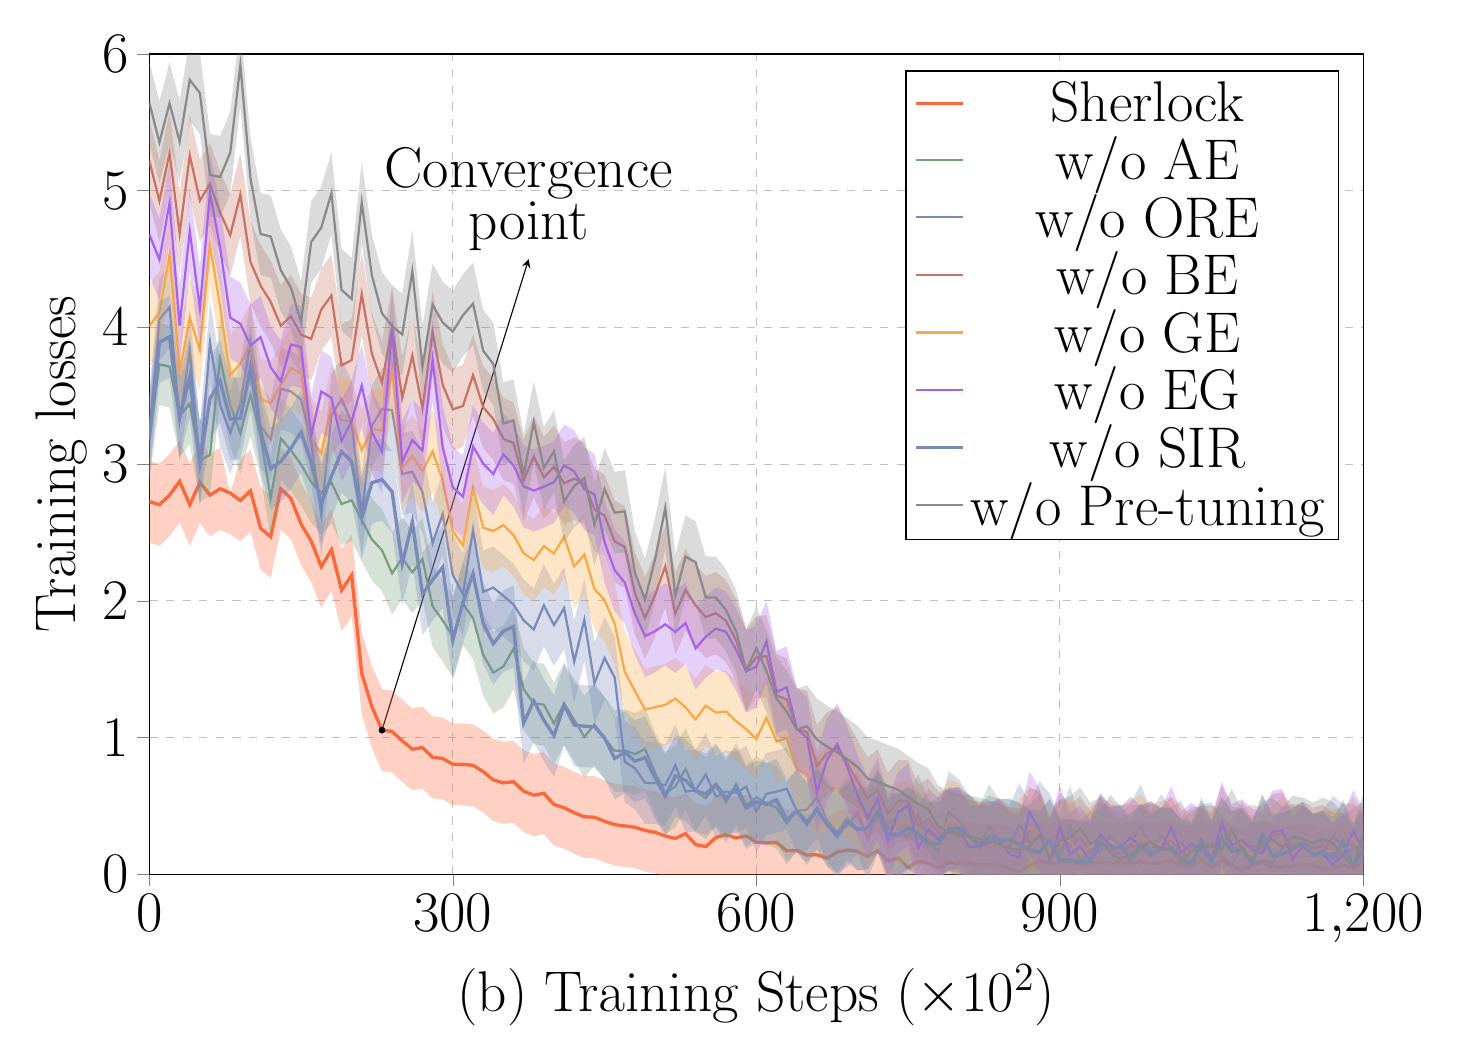
\begin{tikzpicture}
        \footnotesize
        \begin{axis}[
            xmin=0, xmax=1200, % x轴范围
            ymin=0, ymax=6, % y轴范围
            ytick={0, 1, 2, 3, 4, 5, 6},
            xtick={0, 300, 600, 900, 1200, 1500}, % x轴刻度
            xlabel={(b) Training Steps ($\times 10^2$)},
            xlabel style={font=\fontsize{22pt}{28pt}\selectfont},
            ylabel={Training losses},
            ylabel near ticks,
            ylabel style={font=\fontsize{22pt}{28pt}\selectfont},
            legend style={font=\fontsize{22pt}{28pt}\selectfont},
            xtick align=outside,
            ytick align=outside,
            tick label style={font=\fontsize{22pt}{28pt}\selectfont},
            ytick style={font=\fontsize{22pt}{28pt}\selectfont},
            enlargelimits=false,
            xtick pos=bottom,
            ytick pos=left,
            grid=both,
            grid style={dashed},
            width=17cm,
            height=12cm,
            xlabel style={at={(axis description cs:0.5,-0.1)},anchor=north}, % 手动调整xlabel位置
        ]
\addplot [only marks, mark=*, mark size=1pt, forget plot] coordinates {(230,1.0547)};
\draw[-stealth] (axis cs:230,1.0547) -- (axis cs:375,4.5) node[above, align=center] {\fontsize{22pt}{28pt}\selectfont Convergence \\ \fontsize{22pt}{28pt}\selectfont point};
\addplot [
            draw=none, % 不显示边界线
            fill=color3, % 设置阴影颜色
            fill opacity=0.3, % 设置透明度
            domain=0:60,
            samples=100,
            forget plot
        ]
        coordinates {%%add point
(0,3.0266)
(10,3.0031)
(20,3.0734)
(30,3.175)
(40,3.0031)
(50,3.1672)
(60,3.0734)
(70,3.1203)
(80,2.7891)
(90,3.0344)
(100,3.1047)
(110,2.8312)
(120,2.7688)
(130,3.1203)
(140,3.05)
(150,2.8625)
(160,2.7375)
(170,2.55)
(180,2.675)
(190,2.3781)
(200,2.4875)
(210,1.7688)
(220,1.5266)
(230,1.3547)
(240,1.3445)
(250,1.2762)
(260,1.2156)
(270,1.2273)
(280,1.156)
(290,1.148)
(300,1.1048)
(310,1.1043)
(320,1.0978)
(330,1.0516)
(340,0.9906)
(350,0.969)
(360,0.977)
(370,0.9086)
(380,0.8793)
(390,0.893)
(400,0.81)
(410,0.7874)
(420,0.75)
(430,0.721)
(440,0.7177)
(450,0.6883)
(460,0.6631)
(470,0.6543)
(480,0.6445)
(490,0.6211)
(500,0.6074)
(510,0.5801)
(520,0.5625)
(530,0.5977)
(540,0.5176)
(550,0.5029)
(560,0.5684)
(570,0.5902)
(580,0.5658)
(590,0.5814)
(600,0.5355)
(610,0.5297)
(620,0.5326)
(630,0.4721)
(640,0.474)
(650,0.4408)
(660,0.4438)
(670,0.4164)
(680,0.4642)
(690,0.4783)
(700,0.4686)
(710,0.4314)
(720,0.4725)
(730,0.3982)
(740,0.4212)
(750,0.35)
(760,0.3943)
(770,0.3831)
(780,0.3445)
(790,0.3909)
(800,0.3787)
(810,0.3848)
(820,0.3707)
(830,0.3714)
(840,0.3687)
(850,0.3411)
(860,0.3201)
(870,0.3665)
(880,0.3972)
(890,0.3769)
(900,0.3906)
(910,0.3952)
(920,0.3704)
(930,0.3823)
(940,0.3894)
(950,0.382)
(960,0.382)
(970,0.3806)
(980,0.3936)
(990,0.3771)
(1000,0.3837)
(1010,0.3994)
(1020,0.3647)
(1030,0.3587)
(1040,0.4011)
(1050,0.351)
(1060,0.4038)
(1070,0.3599)
(1080,0.3334)
(1090,0.3691)
(1100,0.3903)
(1110,0.3575)
(1120,0.3522)
(1130,0.3596)
(1140,0.3735)
(1150,0.3646)
(1160,0.3341)
(1170,0.3496)
(1180,0.3669)
(1190,0.343)
(1200,0.3925)
(1210,0.3385)
(1220,0.3446)
(1230,0.3404)
(1240,0.3582)
(1250,0.3248)
(1260,0.3498)
(1270,0.3406)
(1280,0.3496)
(1290,0.3615)
(1300,0.3456)
(1310,0.3415)
(1320,0.3366)
(1330,0.3453)
(1340,0.3696)
(1350,0.3464)
(1360,0.3492)
(1370,0.372)
(1380,0.352)
(1390,0.347)
(1400,0.3531)
(1410,0.3253)
(1420,0.3461)
(1430,0.3416)
(1440,0.3619)
(1450,0.3424)
(1460,0.3359)
(1470,0.3361)
(1480,0.3349)
(1490,0.3435)
(1500,0.3521)
(1500,0.0521-0.3)
(1490,0.0435-0.3)
(1480,0.0349-0.3)
(1470,0.0361-0.3)
(1460,0.0359-0.3)
(1450,0.0424-0.3)
(1440,0.0619-0.3)
(1430,0.0416-0.3)
(1420,0.0461-0.3)
(1410,0.0253-0.3)
(1400,0.0531-0.3)
(1390,0.047-0.3)
(1380,0.052-0.3)
(1370,0.072-0.3)
(1360,0.0492-0.3)
(1350,0.0464-0.3)
(1340,0.0696-0.3)
(1330,0.0453-0.3)
(1320,0.0366-0.3)
(1310,0.0415-0.3)
(1300,0.0456-0.3)
(1290,0.0615-0.3)
(1280,0.0496-0.3)
(1270,0.0406-0.3)
(1260,0.0498-0.3)
(1250,0.0248-0.3)
(1240,0.0582-0.3)
(1230,0.0404-0.3)
(1220,0.0446-0.3)
(1210,0.0385-0.3)
(1200,0.0925-0.3)
(1190,0.043-0.3)
(1180,0.0669-0.3)
(1170,0.0496-0.3)
(1160,0.0341-0.3)
(1150,0.0646-0.3)
(1140,0.0735-0.3)
(1130,0.0596-0.3)
(1120,0.0522-0.3)
(1110,0.0575-0.3)
(1100,0.0903-0.3)
(1090,0.0691-0.3)
(1080,0.0334-0.3)
(1070,0.0599-0.3)
(1060,0.1038-0.3)
(1050,0.051-0.3)
(1040,0.1011-0.3)
(1030,0.0587-0.3)
(1020,0.0647-0.3)
(1010,0.0994-0.3)
(1000,0.0837-0.3)
(990,0.0771-0.3)
(980,0.0936-0.3)
(970,0.0806-0.3)
(960,0.082-0.3)
(950,0.082-0.3)
(940,0.0894-0.3)
(930,0.0823-0.3)
(920,0.0704-0.3)
(910,0.0952-0.3)
(900,0.0906-0.3)
(890,0.0769-0.3)
(880,0.0972-0.3)
(870,0.0665-0.3)
(860,0.0201-0.3)
(850,0.0411-0.3)
(840,0.0687-0.3)
(830,0.0714-0.3)
(820,0.0707-0.3)
(810,0.0848-0.3)
(800,0.0787-0.3)
(790,0.0909-0.3)
(780,0.0445-0.3)
(770,0.0831-0.3)
(760,0.0943-0.3)
(750,0.05-0.3)
(740,0.1212-0.3)
(730,0.0982-0.3)
(720,0.1725-0.3)
(710,0.1314-0.3)
(700,0.1686-0.3)
(690,0.1783-0.3)
(680,0.1642-0.3)
(670,0.1164-0.3)
(660,0.1438-0.3)
(650,0.1408-0.3)
(640,0.174-0.3)
(630,0.1721-0.3)
(620,0.2326-0.3)
(610,0.2297-0.3)
(600,0.2355-0.3)
(590,0.2814-0.3)
(580,0.2658-0.3)
(570,0.2902-0.3)
(560,0.2684-0.3)
(550,0.2029-0.3)
(540,0.2176-0.3)
(530,0.2977-0.3)
(520,0.2625-0.3)
(510,0.2801-0.3)
(500,0.3074-0.3)
(490,0.3211-0.3)
(480,0.3445-0.3)
(470,0.3543-0.3)
(460,0.3631-0.3)
(450,0.3883-0.3)
(440,0.4177-0.3)
(430,0.421-0.3)
(420,0.45-0.3)
(410,0.4874-0.3)
(400,0.51-0.3)
(390,0.593-0.3)
(380,0.5793-0.3)
(370,0.6086-0.3)
(360,0.677-0.3)
(350,0.669-0.3)
(340,0.6906-0.3)
(330,0.7516-0.3)
(320,0.7978-0.3)
(310,0.8043-0.3)
(300,0.8048-0.3)
(290,0.848-0.3)
(280,0.856-0.3)
(270,0.9273-0.3)
(260,0.9156-0.3)
(250,0.9762-0.3)
(240,1.0445-0.3)
(230,1.0547-0.3)
(220,1.2266-0.3)
(210,1.4688-0.3)
(200,2.1875-0.3)
(190,2.0781-0.3)
(180,2.375-0.3)
(170,2.25-0.3)
(160,2.4375-0.3)
(150,2.5625-0.3)
(140,2.75-0.3)
(130,2.8203-0.3)
(120,2.4688-0.3)
(110,2.5312-0.3)
(100,2.8047-0.3)
(90,2.7344-0.3)
(80,2.7891-0.3)
(70,2.8203-0.3)
(60,2.7734-0.3)
(50,2.8672-0.3)
(40,2.7031-0.3)
(30,2.875-0.3)
(20,2.7734-0.3)
(10,2.7031-0.3)
(0,2.7266-0.3)


};-- cycle;


\addplot[color=color3,style={very thick}] coordinates{%%GS-LLM
(0,2.7266)
(10,2.7031)
(20,2.7734)
(30,2.875)
(40,2.7031)
(50,2.8672)
(60,2.7734)
(70,2.8203)
(80,2.7891)
(90,2.7344)
(100,2.8047)
(110,2.5312)
(120,2.4688)
(130,2.8203)
(140,2.75)
(150,2.5625)
(160,2.4375)
(170,2.25)
(180,2.375)
(190,2.0781)
(200,2.1875)
(210,1.4688)
(220,1.2266)
(230,1.0547)
(240,1.0445)
(250,0.9762)
(260,0.9156)
(270,0.9273)
(280,0.856)
(290,0.848)
(300,0.8048)
(310,0.8043)
(320,0.7978)
(330,0.7516)
(340,0.6906)
(350,0.669)
(360,0.677)
(370,0.6086)
(380,0.5793)
(390,0.593)
(400,0.51)
(410,0.4874)
(420,0.45)
(430,0.421)
(440,0.4177)
(450,0.3883)
(460,0.3631)
(470,0.3543)
(480,0.3445)
(490,0.3211)
(500,0.3074)
(510,0.2801)
(520,0.2625)
(530,0.2977)
(540,0.2176)
(550,0.2029)
(560,0.2684)
(570,0.2902)
(580,0.2658)
(590,0.2814)
(600,0.2355)
(610,0.2297)
(620,0.2326)
(630,0.1721)
(640,0.174)
(650,0.1408)
(660,0.1438)
(670,0.1164)
(680,0.1642)
(690,0.1783)
(700,0.1686)
(710,0.1314)
(720,0.1725)
(730,0.0982)
(740,0.1212)
(750,0.05)
(760,0.0943)
(770,0.0831)
(780,0.0445)
(790,0.0909)
(800,0.0787)
(810,0.0848)
(820,0.0707)
(830,0.0714)
(840,0.0687)
(850,0.0411)
(860,0.0201)
(870,0.0665)
(880,0.0972)
(890,0.0769)
(900,0.0906)
(910,0.0952)
(920,0.0704)
(930,0.0823)
(940,0.0894)
(950,0.082)
(960,0.082)
(970,0.0806)
(980,0.0936)
(990,0.0771)
(1000,0.0837)
(1010,0.0994)
(1020,0.0647)
(1030,0.0587)
(1040,0.1011)
(1050,0.051)
(1060,0.1038)
(1070,0.0599)
(1080,0.0334)
(1090,0.0691)
(1100,0.0903)
(1110,0.0575)
(1120,0.0522)
(1130,0.0596)
(1140,0.0735)
(1150,0.0646)
(1160,0.0341)
(1170,0.0496)
(1180,0.0669)
(1190,0.043)
(1200,0.0925)
(1210,0.0385)
(1220,0.0446)
(1230,0.0404)
(1240,0.0582)
(1250,0.0248)
(1260,0.0498)
(1270,0.0406)
(1280,0.0496)
(1290,0.0615)
(1300,0.0456)
(1310,0.0415)
(1320,0.0366)
(1330,0.0453)
(1340,0.0696)
(1350,0.0464)
(1360,0.0492)
(1370,0.072)
(1380,0.052)
(1390,0.047)
(1400,0.0531)
(1410,0.0253)
(1420,0.0461)
(1430,0.0416)
(1440,0.0619)
(1450,0.0424)
(1460,0.0359)
(1470,0.0361)
(1480,0.0349)
(1490,0.0435)
(1500,0.0521)};

\addplot [
            draw=none, % 不显示边界线
            fill=color1, % 设置阴影颜色
            fill opacity=0.3, % 设置透明度
            domain=0:60,
            samples=100,
            forget plot
        ]
        coordinates {%%add pointcoordinates{%%woae
(0,3.480114493881013)
(10,4.030598897770529)
(20,4.0128897662559766)
(30,3.653333145432956)
(40,3.7425186224121975)
(50,3.325071153902197)
(60,3.3683550085043754)
(70,4.075631044348548)
(80,3.7328368556086275)
(90,3.527421795882818)
(100,3.8074179956206972)
(110,3.503013619168705)
(120,3.051981252127913)
(130,3.487413102668993)
(140,3.401799205361271)
(150,3.29768764245908)
(160,3.169143032526988)
(170,3.0879855195516447)
(180,3.164982891665143)
(190,3.008576910536783)
(200,3.0359475885104323)
(210,2.889698902029306)
(220,2.750139632061747)
(230,2.6705626925048656)
(240,2.5008461403811444)
(250,2.6148310897012502)
(260,2.5083261115204929)
(270,2.6050980391537358)
(280,2.2611508772230333)
(290,2.1571158326295372)
(300,2.0413586117350553)
(310,2.2788909087698864)
(320,2.1735942964534253)
(330,1.9062925230839892)
(340,1.775847590144245)
(350,1.8204095801024901)
(360,1.9520723388100848)
(370,1.6549416297263261)
(380,1.551030048113351)
(390,1.5412056052850896)
(400,1.4034344586851495)
(410,1.5492934175841121)
(420,1.4292441472933247)
(430,1.3051646483681112)
(440,1.3962971095255313)
(450,1.2976611334578196)
(460,1.2035206191197932)
(470,1.2058418749370752)
(480,1.179773785692016)
(490,1.2169967290539324)
(500,1.0406335258361159)
(510,0.8944158858768556)
(520,0.9433163679823175)
(530,1.0709910190347978)
(540,0.9074449008391298)
(550,0.8579701219570895)
(560,0.9464510461803418)
(570,0.8286364732350024)
(580,0.9608769016333534)
(590,0.8025217492800271)
(600,0.863718812671316)
(610,0.8194777496675899)
(620,0.78815815616524155)
(630,0.67282744089998243)
(640,0.7653292736380306)
(650,0.6866861399811182)
(660,0.78502965847619894)
(670,0.6539845226493228)
(680,0.6103148887647507)
(690,0.71561240228664426)
(700,0.6283367298083043)
(710,0.6311302561616555)
(720,0.7586115504877433)
(730,0.6453209766226401)
(740,0.5841270005318454)
(750,0.63905682216959965)
(760,0.5761610311679017)
(770,0.50739571298827061)
(780,0.5734049047314774)
(790,0.63220913894107995)
(800,0.6332537560876506)
(810,0.5791434559750482)
(820,0.48935533585741932)
(830,0.65958730586186294)
(840,0.54785215369122598)
(850,0.55282671808045615)
(860,0.51963500219480386)
(870,0.47959543070282266)
(880,0.45841831833205788)
(890,0.5573381316146617)
(900,0.39992651739745835)
(910,0.40408090647983746)
(920,0.38723575707561694)
(930,0.39411736261886593)
(940,0.5864417225718713)
(950,0.5047118481870152)
(960,0.5101886185592684)
(970,0.382098588762447)
(980,0.48923385021939843)
(990,0.43175695270180887)
(1000,0.48655301924047166)
(1010,0.4862203547749958)
(1020,0.39984879288589278)
(1030,0.36259332780311236)
(1040,0.5639653906508713)
(1050,0.387918164630465)
(1060,0.5673709087715913)
(1070,0.46305151207623447)
(1080,0.47118550639140162)
(1090,0.37537670297424534)
(1100,0.5777879905662321)
(1110,0.43680946961505805)
(1120,0.44369401909475604)
(1130,0.4807266898164753)
(1140,0.52709230382520973)
(1150,0.43825348545227395)
(1160,0.46040681752450592)
(1170,0.35662009127081713)
(1180,0.55062279538380633)
(1190,0.36273137347052898)
(1200,0.51916387830659656)
(1210,0.45067372855274402)
(1220,0.42700535846640285)
(1230,0.358639376494203706)
(1240,0.37486480634803964)
(1250,0.43626515442177986)
(1260,0.3847955898157942)
(1270,0.36705913704092291)
(1280,0.37919160855448171)
(1290,0.4919752447175208)
(1300,0.48598820376855243)
(1310,0.37678520053956177)
(1320,0.46270057505316834)
(1330,0.3565483390539744)
(1340,0.4817031618595632)
(1350,0.51344691362675028)
(1360,0.48193554830826128)
(1370,0.5668417064718476)
(1380,0.53401321130133584)
(1390,0.4630847949705197)
(1400,0.45285661320373375)
(1410,0.36200894956604644)
(1420,0.54289963907898074)
(1430,0.44729723678088952)
(1440,0.55060126348390604)
(1450,0.4378212462992232)
(1460,0.52544468588022876)
(1470,0.44188022678836126)
(1480,0.4829810364748377)
(1490,0.46055819951119044)
(1500,0.48253543894129504)
(1500,0.18253543894129504-0.3)
(1490,0.16055819951119044-0.3)
(1480,0.1829810364748377-0.3)
(1470,0.14188022678836126-0.3)
(1460,0.22544468588022876-0.3)
(1450,0.1378212462992232-0.3)
(1440,0.25060126348390604-0.3)
(1430,0.14729723678088952-0.3)
(1420,0.24289963907898074-0.3)
(1410,0.06200894956604644-0.3)
(1400,0.15285661320373375-0.3)
(1390,0.1630847949705197-0.3)
(1380,0.23401321130133584-0.3)
(1370,0.2668417064718476-0.3)
(1360,0.18193554830826128-0.3)
(1350,0.21344691362675028-0.3)
(1340,0.1817031618595632-0.3)
(1330,0.0565483390539744-0.3)
(1320,0.16270057505316834-0.3)
(1310,0.07678520053956177-0.3)
(1300,0.18598820376855243-0.3)
(1290,0.1919752447175208-0.3)
(1280,0.07919160855448171-0.3)
(1270,0.06705913704092291-0.3)
(1260,0.0847955898157942-0.3)
(1250,0.13626515442177986-0.3)
(1240,0.07486480634803964-0.3)
(1230,0.058639376494203706-0.3)
(1220,0.12700535846640285-0.3)
(1210,0.15067372855274402-0.3)
(1200,0.21916387830659656-0.3)
(1190,0.06273137347052898-0.3)
(1180,0.25062279538380633-0.3)
(1170,0.05662009127081713-0.3)
(1160,0.16040681752450592-0.3)
(1150,0.13825348545227395-0.3)
(1140,0.22709230382520973-0.3)
(1130,0.1807266898164753-0.3)
(1120,0.14369401909475604-0.3)
(1110,0.13680946961505805-0.3)
(1100,0.2777879905662321-0.3)
(1090,0.07537670297424534-0.3)
(1080,0.17118550639140162-0.3)
(1070,0.16305151207623447-0.3)
(1060,0.2673709087715913-0.3)
(1050,0.087918164630465-0.3)
(1040,0.2639653906508713-0.3)
(1030,0.06259332780311236-0.3)
(1020,0.09984879288589278-0.3)
(1010,0.1862203547749958-0.3)
(1000,0.18655301924047166-0.3)
(990,0.13175695270180887-0.3)
(980,0.18923385021939843-0.3)
(970,0.082098588762447-0.3)
(960,0.2101886185592684-0.3)
(950,0.2047118481870152-0.3)
(940,0.2864417225718713-0.3)
(930,0.09411736261886593-0.3)
(920,0.08723575707561694-0.3)
(910,0.10408090647983746-0.3)
(900,0.09992651739745835-0.3)
(890,0.2573381316146617-0.3)
(880,0.15841831833205788-0.3)
(870,0.17959543070282266-0.3)
(860,0.21963500219480386-0.3)
(850,0.25282671808045615-0.3)
(840,0.24785215369122598-0.3)
(830,0.35958730586186294-0.3)
(820,0.18935533585741932-0.3)
(810,0.2791434559750482-0.3)
(800,0.2832537560876506-0.3)
(790,0.33220913894107995-0.3)
(780,0.2734049047314774-0.3)
(770,0.20739571298827061-0.3)
(760,0.2761610311679017-0.3)
(750,0.33905682216959965-0.3)
(740,0.2841270005318454-0.3)
(730,0.3453209766226401-0.3)
(720,0.4586115504877433-0.3)
(710,0.3311302561616555-0.3)
(700,0.3283367298083043-0.3)
(690,0.41561240228664426-0.3)
(680,0.3103148887647507-0.3)
(670,0.3539845226493228-0.3)
(660,0.48502965847619894-0.3)
(650,0.3866861399811182-0.3)
(640,0.4653292736380306-0.3)
(630,0.37282744089998243-0.3)
(620,0.48815815616524155-0.3)
(610,0.5194777496675899-0.3)
(600,0.563718812671316-0.3)
(590,0.5025217492800271-0.3)
(580,0.6608769016333534-0.3)
(570,0.5286364732350024-0.3)
(560,0.6464510461803418-0.3)
(550,0.5579701219570895-0.3)
(540,0.6074449008391298-0.3)
(530,0.7709910190347978-0.3)
(520,0.6433163679823175-0.3)
(510,0.5944158858768556-0.3)
(500,0.7406335258361159-0.3)
(490,0.9169967290539324-0.3)
(480,0.879773785692016-0.3)
(470,0.9058418749370752-0.3)
(460,0.9035206191197932-0.3)
(450,0.9976611334578196-0.3)
(440,1.0962971095255313-0.3)
(430,1.0051646483681112-0.3)
(420,1.1292441472933247-0.3)
(410,1.2492934175841121-0.3)
(400,1.1034344586851495-0.3)
(390,1.2412056052850896-0.3)
(380,1.251030048113351-0.3)
(370,1.3549416297263261-0.3)
(360,1.6520723388100848-0.3)
(350,1.5204095801024901-0.3)
(340,1.475847590144245-0.3)
(330,1.6062925230839892-0.3)
(320,1.8735942964534253-0.3)
(310,1.9788909087698864-0.3)
(300,1.7413586117350553-0.3)
(290,1.8571158326295372-0.3)
(280,1.9611508772230333-0.3)
(270,2.3050980391537358-0.3)
(260,2.2083261115204929-0.3)
(250,2.3148310897012502-0.3)
(240,2.2008461403811444-0.3)
(230,2.3705626925048656-0.3)
(220,2.450139632061747-0.3)
(210,2.589698902029306-0.3)
(200,2.7359475885104323-0.3)
(190,2.708576910536783-0.3)
(180,2.864982891665143-0.3)
(170,2.7879855195516447-0.3)
(160,2.869143032526988-0.3)
(150,2.99768764245908-0.3)
(140,3.101799205361271-0.3)
(130,3.187413102668993-0.3)
(120,2.751981252127913-0.3)
(110,3.203013619168705-0.3)
(100,3.5074179956206972-0.3)
(90,3.227421795882818-0.3)
(80,3.4328368556086275-0.3)
(70,3.775631044348548-0.3)
(60,3.0683550085043754-0.3)
(50,3.025071153902197-0.3)
(40,3.4425186224121975-0.3)
(30,3.353333145432956-0.3)
(20,3.7128897662559766-0.3)
(10,3.730598897770529-0.3)
(0,3.180114493881013-0.3)

};
\addplot[color=color1,style={thick}] coordinates{
%%woae
(0,3.180114493881013)
(10,3.730598897770529)
(20,3.7128897662559766)
(30,3.353333145432956)
(40,3.4425186224121975)
(50,3.025071153902197)
(60,3.0683550085043754)
(70,3.775631044348548)
(80,3.4328368556086275)
(90,3.227421795882818)
(100,3.5074179956206972)
(110,3.203013619168705)
(120,2.751981252127913)
(130,3.187413102668993)
(140,3.101799205361271)
(150,2.99768764245908)
(160,2.869143032526988)
(170,2.7879855195516447)
(180,2.864982891665143)
(190,2.708576910536783)
(200,2.7359475885104323)
(210,2.589698902029306)
(220,2.450139632061747)
(230,2.3705626925048656)
(240,2.2008461403811444)
(250,2.3148310897012502)
(260,2.2083261115204929)
(270,2.3050980391537358)
(280,1.9611508772230333)
(290,1.8571158326295372)
(300,1.7413586117350553)
(310,1.9788909087698864)
(320,1.8735942964534253)
(330,1.6062925230839892)
(340,1.475847590144245)
(350,1.5204095801024901)
(360,1.6520723388100848)
(370,1.3549416297263261)
(380,1.251030048113351)
(390,1.2412056052850896)
(400,1.1034344586851495)
(410,1.2492934175841121)
(420,1.1292441472933247)
(430,1.0051646483681112)
(440,1.0962971095255313)
(450,0.9976611334578196)
(460,0.9035206191197932)
(470,0.9058418749370752)
(480,0.879773785692016)
(490,0.9169967290539324)
(500,0.7406335258361159)
(510,0.5944158858768556)
(520,0.6433163679823175)
(530,0.7709910190347978)
(540,0.6074449008391298)
(550,0.5579701219570895)
(560,0.6464510461803418)
(570,0.5286364732350024)
(580,0.6608769016333534)
(590,0.5025217492800271)
(600,0.563718812671316)
(610,0.5194777496675899)
(620,0.48815815616524155)
(630,0.37282744089998243)
(640,0.4653292736380306)
(650,0.3866861399811182)
(660,0.48502965847619894)
(670,0.3539845226493228)
(680,0.3103148887647507)
(690,0.41561240228664426)
(700,0.3283367298083043)
(710,0.3311302561616555)
(720,0.4586115504877433)
(730,0.3453209766226401)
(740,0.2841270005318454)
(750,0.33905682216959965)
(760,0.2761610311679017)
(770,0.20739571298827061)
(780,0.2734049047314774)
(790,0.33220913894107995)
(800,0.2832537560876506)
(810,0.2791434559750482)
(820,0.18935533585741932)
(830,0.35958730586186294)
(840,0.24785215369122598)
(850,0.25282671808045615)
(860,0.21963500219480386)
(870,0.17959543070282266)
(880,0.15841831833205788)
(890,0.2573381316146617)
(900,0.09992651739745835)
(910,0.10408090647983746)
(920,0.08723575707561694)
(930,0.09411736261886593)
(940,0.2864417225718713)
(950,0.2047118481870152)
(960,0.2101886185592684)
(970,0.082098588762447)
(980,0.18923385021939843)
(990,0.13175695270180887)
(1000,0.18655301924047166)
(1010,0.1862203547749958)
(1020,0.09984879288589278)
(1030,0.06259332780311236)
(1040,0.2639653906508713)
(1050,0.087918164630465)
(1060,0.2673709087715913)
(1070,0.16305151207623447)
(1080,0.17118550639140162)
(1090,0.07537670297424534)
(1100,0.2777879905662321)
(1110,0.13680946961505805)
(1120,0.14369401909475604)
(1130,0.1807266898164753)
(1140,0.22709230382520973)
(1150,0.13825348545227395)
(1160,0.16040681752450592)
(1170,0.05662009127081713)
(1180,0.25062279538380633)
(1190,0.06273137347052898)
(1200,0.21916387830659656)
(1210,0.15067372855274402)
(1220,0.12700535846640285)
(1230,0.058639376494203706)
(1240,0.07486480634803964)
(1250,0.13626515442177986)
(1260,0.0847955898157942)
(1270,0.06705913704092291)
(1280,0.07919160855448171)
(1290,0.1919752447175208)
(1300,0.18598820376855243)
(1310,0.07678520053956177)
(1320,0.16270057505316834)
(1330,0.0565483390539744)
(1340,0.1817031618595632)
(1350,0.21344691362675028)
(1360,0.18193554830826128)
(1370,0.2668417064718476)
(1380,0.23401321130133584)
(1390,0.1630847949705197)
(1400,0.15285661320373375)
(1410,0.06200894956604644)
(1420,0.24289963907898074)
(1430,0.14729723678088952)
(1440,0.25060126348390604)
(1450,0.1378212462992232)
(1460,0.22544468588022876)
(1470,0.14188022678836126)
(1480,0.1829810364748377)
(1490,0.16055819951119044)
(1500,0.18253543894129504)
};
\addplot [
            draw=none, % 不显示边界线
            fill=color5, % 设置阴影颜色
            fill opacity=0.3, % 设置透明度
            domain=0:60,
            samples=100,
            forget plot
        ]
        coordinates {
(0,3.5141290705883088)
(10,4.357594887738707)
(20,4.4487870246078415)
(30,3.620773610261464)
(40,4.1380012784236426)
(50,3.2822819511341336)
(60,4.1904355231720595)
(70,3.7324039106589392)
(80,3.5289397324977713)
(90,3.7415178823986747)
(100,4.189861400504425)
(110,3.5785407998741474)
(120,3.480577670812488)
(130,3.8513297309115077)
(140,3.831729423639607)
(150,3.772856025804918)
(160,3.4639412631520347)
(170,2.930193591936108)
(180,3.656555042188535)
(190,3.775715171672767)
(200,3.6062247366530593)
(210,2.929383934248947)
(220,3.5792889715591804)
(230,3.703698046045783)
(240,3.6945962524466726)
(250,3.2275684233257309)
(260,3.2449418653001612)
(270,3.096231635277644)
(280,2.7231270744210166)
(290,2.9351348991559713)
(300,2.4900724103473054)
(310,2.348674053011612)
(320,2.8243198482888172)
(330,2.3657721790281491)
(340,2.3975922734788124)
(350,2.3369489264964622)
(360,2.273488240519922)
(370,2.1581546890208421)
(380,2.0910880611281695)
(390,2.2675088032791241)
(400,2.1232478647984157)
(410,2.2468757098396731)
(420,1.8558070384964361)
(430,2.1614622374465108)
(440,1.6980176469908279)
(450,1.8822932223382747)
(460,1.7393686659154372)
(470,1.1227941444152618)
(480,1.0759610357907828)
(490,0.969816263942634)
(500,0.9676524832549956)
(510,0.9512292532123187)
(520,1.09700072496078)
(530,0.9058325600472404)
(540,0.9140291916651753)
(550,1.0311219627573777)
(560,0.8684640502157361)
(570,0.9067217547310451)
(580,0.8966294133031911)
(590,0.9408342431042785)
(600,0.7611624257946794)
(610,0.8888002259654523)
(620,0.9055670949384334)
(630,0.9263180697673764)
(640,0.76415791940045514)
(650,0.7738224676544774)
(660,0.8632626176004553)
(670,0.6942445013131637)
(680,0.6059398933197375)
(690,0.6545437512482949)
(700,0.75054693003678004)
(710,0.55580408092465545)
(720,0.756656583076731)
(730,0.545430813796496)
(740,0.5911950695543999)
(750,0.5700094603467655)
(760,0.7349634992967786)
(770,0.54777740396869752)
(780,0.4652064524791081)
(790,0.7555425089770313)
(800,0.6955555368484442)
(810,0.58351874108760644)
(820,0.52644073835306056)
(830,0.49375054888552304)
(840,0.5537689675519195)
(850,0.50159736238580528)
(860,0.66659527099007794)
(870,0.52589201862465635)
(880,0.683747960648798)
(890,0.58795396083080889)
(900,0.43258153319440333)
(910,0.6482386083600343)
(920,0.39796771126741109)
(930,0.4610422914664913)
(940,0.46399277325155637)
(950,0.58242959042419324)
(960,0.49896545588127768)
(970,0.52122800108829863)
(980,0.66038932913242244)
(990,0.46288055763596482)
(1000,0.58300186281734185)
(1010,0.49342918799296815)
(1020,0.5395058813856895)
(1030,0.36018966836381871)
(1040,0.51554900290372658)
(1050,0.52422428612233475)
(1060,0.4287757359309475)
(1070,0.36341059338973612)
(1080,0.52021623991955186)
(1090,0.38742231942997614)
(1100,0.4005238621194955)
(1110,0.38579176053199668)
(1120,0.49331370122139888)
(1130,0.51569132290106807)
(1140,0.49758608312223502)
(1150,0.44048019093619524)
(1160,0.47041507172424245)
(1170,0.57248815901754303)
(1180,0.51488410368166944)
(1190,0.51888576573252472)
(1200,0.43567382125473046)
(1210,0.59669614153897436)
(1220,0.42681876018944355)
(1230,0.5397084670090236)
(1240,0.53329862815507088)
(1250,0.5775612475292919)
(1260,0.3957420411767668)
(1270,0.48596105178153974)
(1280,0.5509267423871523)
(1290,0.36823140666475526)
(1300,0.48347474670939473)
(1310,0.5721519432638145)
(1320,0.37400748931798753)
(1330,0.5607579030341154)
(1340,0.53891520867519983)
(1350,0.43487207904339266)
(1360,0.44784805885601823)
(1370,0.57343489310841995)
(1380,0.5574466816290006)
(1390,0.61236252283897303)
(1400,0.4904622529659748)
(1410,0.34143395228188508)
(1420,0.50259441274448542)
(1430,0.509924029719852)
(1440,0.37127899171289406)
(1450,0.40364755524281688)
(1460,0.5844559761959343)
(1470,0.3676633983533227)
(1480,0.54651837602884458)
(1490,0.4961956385477216)
(1500,0.54517823859903357)
(1500, 0.24517823859903357 - 0.3)
(1490, 0.1961956385477216 - 0.3)
(1480, 0.24651837602884458 - 0.3)
(1470, 0.1676633983533227 - 0.3)
(1460, 0.2844559761959343 - 0.3)
(1450, 0.10364755524281688 - 0.3)
(1440, 0.07127899171289406 - 0.3)
(1430, 0.209924029719852 - 0.3)
(1420, 0.20259441274448542 - 0.3)
(1410, 0.04143395228188508 - 0.3)
(1400, 0.1904622529659748 - 0.3)
(1390, 0.31236252283897303 - 0.3)
(1380, 0.2574466816290006 - 0.3)
(1370, 0.27343489310841995 - 0.3)
(1360, 0.14784805885601823 - 0.3)
(1350, 0.13487207904339266 - 0.3)
(1340, 0.23891520867519983 - 0.3)
(1330, 0.2607579030341154 - 0.3)
(1320, 0.07400748931798753 - 0.3)
(1310, 0.2721519432638145 - 0.3)
(1300, 0.18347474670939473 - 0.3)
(1290, 0.06823140666475526 - 0.3)
(1280, 0.2509267423871523 - 0.3)
(1270, 0.18596105178153974 - 0.3)
(1260, 0.0957420411767668 - 0.3)
(1250, 0.2775612475292919 - 0.3)
(1240, 0.23329862815507088 - 0.3)
(1230, 0.2397084670090236 - 0.3)
(1220, 0.12681876018944355 - 0.3)
(1210, 0.19669614153897436 - 0.3)
(1200, 0.13567382125473046 - 0.3)
(1190, 0.21888576573252472 - 0.3)
(1180, 0.21488410368166944 - 0.3)
(1170, 0.27248815901754303 - 0.3)
(1160, 0.17041507172424245 - 0.3)
(1150, 0.14048019093619524 - 0.3)
(1140, 0.19758608312223502 - 0.3)
(1130, 0.21569132290106807 - 0.3)
(1120, 0.19331370122139888 - 0.3)
(1110, 0.08579176053199668 - 0.3)
(1100, 0.1005238621194955 - 0.3)
(1090, 0.08742231942997614 - 0.3)
(1080, 0.22021623991955186 - 0.3)
(1070, 0.06341059338973612 - 0.3)
(1060, 0.1287757359309475 - 0.3)
(1050, 0.22422428612233475 - 0.3)
(1040, 0.21554900290372658 - 0.3)
(1030, 0.06018966836381871 - 0.3)
(1020, 0.2395058813856895 - 0.3)
(1010, 0.19342918799296815 - 0.3)
(1000, 0.28300186281734185 - 0.3)
(990, 0.16288055763596482 - 0.3)
(980, 0.36038932913242244 - 0.3)
(970, 0.22122800108829863 - 0.3)
(960, 0.19896545588127768 - 0.3)
(950, 0.28242959042419324 - 0.3)
(940, 0.16399277325155637 - 0.3)
(930, 0.1610422914664913 - 0.3)
(920, 0.09796771126741109 - 0.3)
(910, 0.3482386083600343 - 0.3)
(900, 0.13258153319440333 - 0.3)
(890, 0.23795396083080889 - 0.3)
(880, 0.283747960648798 - 0.3)
(870, 0.22589201862465635 - 0.3)
(860, 0.36659527099007794 - 0.3)
(850, 0.20159736238580528 - 0.3)
(840, 0.2537689675519195 - 0.3)
(830, 0.19375054888552304 - 0.3)
(820, 0.22644073835306056 - 0.3)
(810, 0.28351874108760644 - 0.3)
(800, 0.3955555368484442 - 0.3)
(790, 0.4555425089770313 - 0.3)
(780, 0.1652064524791081 - 0.3)
(770, 0.24777740396869752 - 0.3)
(760, 0.4349634992967786 - 0.3)
(750, 0.2700094603467655 - 0.3)
(740, 0.2911950695543999 - 0.3)
(730, 0.245430813796496 - 0.3)
(720, 0.456656583076731 - 0.3)
(710, 0.25580408092465545 - 0.3)
(700, 0.45054693003678004 - 0.3)
(690, 0.3545437512482949 - 0.3)
(680, 0.3059398933197375 - 0.3)
(670, 0.3942445013131637 - 0.3)
(660, 0.5632626176004553 - 0.3)
(650, 0.4738224676544774 - 0.3)
(640, 0.46415791940045514 - 0.3)
(630, 0.6263180697673764 - 0.3)
(620, 0.6055670949384334 - 0.3)
(610, 0.5888002259654523 - 0.3)
(600, 0.4611624257946794 - 0.3)
(590, 0.6408342431042785 - 0.3)
(580, 0.5966294133031911 - 0.3)
(570, 0.6067217547310451 - 0.3)
(560, 0.5684640502157361 - 0.3)
(550, 0.7311219627573777 - 0.3)
(540, 0.6140291916651753 - 0.3)
(530, 0.6058325600472404 - 0.3)
(520, 0.79700072496078 - 0.3)
(510, 0.6512292532123187 - 0.3)
(500, 0.6676524832549956 - 0.3)
(490, 0.669816263942634 - 0.3)
(480, 0.7759610357907828 - 0.3)
(470, 0.8227941444152618 - 0.3)
(460, 1.4393686659154372 - 0.3)
(450, 1.5822932223382747 - 0.3)
(440, 1.3980176469908279 - 0.3)
(430, 1.8614622374465108 - 0.3)
(420, 1.5558070384964361 - 0.3)
(410, 1.9468757098396731 - 0.3)
(400, 1.8232478647984157 - 0.3)
(390, 1.9675088032791241 - 0.3)
(380, 1.7910880611281695 - 0.3)
(370, 1.8581546890208421 - 0.3)
(360, 1.973488240519922 - 0.3)
(350, 2.0369489264964622 - 0.3)
(340, 2.0975922734788124 - 0.3)
(330, 2.0657721790281491 - 0.3)
(320, 2.5243198482888172 - 0.3)
(310, 2.048674053011612 - 0.3)
(300, 2.1900724103473054 - 0.3)
(290, 2.6351348991559713 - 0.3)
(280, 2.4231270744210166 - 0.3)
(270, 2.796231635277644 - 0.3)
(260, 2.9449418653001612 - 0.3)
(250, 2.9275684233257309 - 0.3)
(240, 3.3945962524466726 - 0.3)
(230, 3.403698046045783 - 0.3)
(220, 3.2792889715591804 - 0.3)
(210, 2.629383934248947 - 0.3)
(200, 3.3062247366530593 - 0.3)
(190, 3.475715171672767 - 0.3)
(180, 3.356555042188535 - 0.3)
(170, 2.630193591936108 - 0.3)
(160, 3.1639412631520347 - 0.3)
(150, 3.472856025804918 - 0.3)
(140, 3.531729423639607 - 0.3)
(130, 3.5513297309115077 - 0.3)
(120, 3.180577670812488 - 0.3)
(110, 3.2785407998741474 - 0.3)
(100, 3.889861400504425 - 0.3)
(90, 3.4415178823986747 - 0.3)
(80, 3.2289397324977713 - 0.3)
(70, 3.4324039106589392 - 0.3)
(60, 3.8904355231720595 - 0.3)
(50, 2.9822819511341336 - 0.3)
(40, 3.8380012784236426 - 0.3)
(30, 3.320773610261464 - 0.3)
(20, 4.1487870246078415 - 0.3)
(10, 4.057594887738707 - 0.3)
(0, 3.2141290705883088 - 0.3)
        };
\addplot[color=color5,style={thick}] coordinates{
%%woore
(0,3.2141290705883088)
(10,4.057594887738707)
(20,4.1487870246078415)
(30,3.320773610261464)
(40,3.8380012784236426)
(50,2.9822819511341336)
(60,3.8904355231720595)
(70,3.4324039106589392)
(80,3.2289397324977713)
(90,3.4415178823986747)
(100,3.889861400504425)
(110,3.2785407998741474)
(120,3.180577670812488)
(130,3.5513297309115077)
(140,3.531729423639607)
(150,3.472856025804918)
(160,3.1639412631520347)
(170,2.630193591936108)
(180,3.356555042188535)
(190,3.475715171672767)
(200,3.3062247366530593)
(210,2.629383934248947)
(220,3.2792889715591804)
(230,3.403698046045783)
(240,3.3945962524466726)
(250,2.9275684233257309)
(260,2.9449418653001612)
(270,2.796231635277644)
(280,2.4231270744210166)
(290,2.6351348991559713)
(300,2.1900724103473054)
(310,2.048674053011612)
(320,2.5243198482888172)
(330,2.0657721790281491)
(340,2.0975922734788124)
(350,2.0369489264964622)
(360,1.973488240519922)
(370,1.8581546890208421)
(380,1.7910880611281695)
(390,1.9675088032791241)
(400,1.8232478647984157)
(410,1.9468757098396731)
(420,1.5558070384964361)
(430,1.8614622374465108)
(440,1.3980176469908279)
(450,1.5822932223382747)
(460,1.4393686659154372)
(470,0.8227941444152618)
(480,0.7759610357907828)
(490,0.669816263942634)
(500,0.6676524832549956)
(510,0.6512292532123187)
(520,0.79700072496078)
(530,0.6058325600472404)
(540,0.6140291916651753)
(550,0.7311219627573777)
(560,0.5684640502157361)
(570,0.6067217547310451)
(580,0.5966294133031911)
(590,0.6408342431042785)
(600,0.4611624257946794)
(610,0.5888002259654523)
(620,0.6055670949384334)
(630,0.6263180697673764)
(640,0.46415791940045514)
(650,0.4738224676544774)
(660,0.5632626176004553)
(670,0.3942445013131637)
(680,0.3059398933197375)
(690,0.3545437512482949)
(700,0.45054693003678004)
(710,0.25580408092465545)
(720,0.456656583076731)
(730,0.245430813796496)
(740,0.2911950695543999)
(750,0.2700094603467655)
(760,0.4349634992967786)
(770,0.24777740396869752)
(780,0.1652064524791081)
(790,0.4555425089770313)
(800,0.3955555368484442)
(810,0.28351874108760644)
(820,0.22644073835306056)
(830,0.19375054888552304)
(840,0.2537689675519195)
(850,0.20159736238580528)
(860,0.36659527099007794)
(870,0.22589201862465635)
(880,0.283747960648798)
(890,0.23795396083080889)
(900,0.13258153319440333)
(910,0.3482386083600343)
(920,0.09796771126741109)
(930,0.1610422914664913)
(940,0.16399277325155637)
(950,0.28242959042419324)
(960,0.19896545588127768)
(970,0.22122800108829863)
(980,0.36038932913242244)
(990,0.16288055763596482)
(1000,0.28300186281734185)
(1010,0.19342918799296815)
(1020,0.2395058813856895)
(1030,0.06018966836381871)
(1040,0.21554900290372658)
(1050,0.22422428612233475)
(1060,0.1287757359309475)
(1070,0.06341059338973612)
(1080,0.22021623991955186)
(1090,0.08742231942997614)
(1100,0.1005238621194955)
(1110,0.08579176053199668)
(1120,0.19331370122139888)
(1130,0.21569132290106807)
(1140,0.19758608312223502)
(1150,0.14048019093619524)
(1160,0.17041507172424245)
(1170,0.27248815901754303)
(1180,0.21488410368166944)
(1190,0.21888576573252472)
(1200,0.13567382125473046)
(1210,0.19669614153897436)
(1220,0.12681876018944355)
(1230,0.2397084670090236)
(1240,0.23329862815507088)
(1250,0.2775612475292919)
(1260,0.0957420411767668)
(1270,0.18596105178153974)
(1280,0.2509267423871523)
(1290,0.06823140666475526)
(1300,0.18347474670939473)
(1310,0.2721519432638145)
(1320,0.07400748931798753)
(1330,0.2607579030341154)
(1340,0.23891520867519983)
(1350,0.13487207904339266)
(1360,0.14784805885601823)
(1370,0.27343489310841995)
(1380,0.2574466816290006)
(1390,0.31236252283897303)
(1400,0.1904622529659748)
(1410,0.04143395228188508)
(1420,0.20259441274448542)
(1430,0.209924029719852)
(1440,0.07127899171289406)
(1450,0.10364755524281688)
(1460,0.2844559761959343)
(1470,0.1676633983533227)
(1480,0.24651837602884458)
(1490,0.1961956385477216)
(1500,0.24517823859903357)
};

\addplot [
            draw=none, % 不显示边界线
            fill=color2, % 设置阴影颜色
            fill opacity=0.3, % 设置透明度
            domain=0:60,
            samples=100,
            forget plot
        ]
        coordinates {

(0,5.51985410814166)
(10,5.224752967168221)
(20,5.575377809212395)
(30,4.986641440392091)
(40,5.557692266696784)
(50,5.226985029365087)
(60,5.349919084826661)
(70,5.14109601191063)
(80,4.975237692300241)
(90,5.272355196291334)
(100,4.77971686360013)
(110,4.606275972670328)
(120,4.486561618868999)
(130,4.311589563112186)
(140,4.383251698581911)
(150,4.247692624222688)
(160,4.216062714729572)
(170,4.430936953683771)
(180,4.53355298192587)
(190,4.022417809840279)
(200,4.061665424957632)
(210,4.543958122007015)
(220,4.108207905761148)
(230,3.8973138180828425)
(240,4.300275261069383)
(250,3.783167079365237)
(260,4.093756631464423)
(270,3.706691000834929)
(280,4.266408517406947)
(290,3.879805226124065)
(300,3.7007645358599876)
(310,3.725413259975993)
(320,3.9520271725524062)
(330,3.717282965226259)
(340,3.630718687267823)
(350,3.4844618824174834)
(360,3.4555503263467623)
(370,3.1794966285182012)
(380,3.3560198436310783)
(390,3.2035999107498997)
(400,3.281459917417847)
(410,3.15942724504647)
(420,3.1938282191911988)
(430,3.1581975630799117)
(440,2.967956107513184)
(450,2.923766403506485)
(460,2.734616674311991)
(470,2.694136926758883)
(480,2.3569419404227673)
(490,2.175264634954178)
(500,2.3438450813203747)
(510,2.5538732878760082)
(520,2.206565969582932)
(530,2.38061582570942)
(540,2.2673591970604955)
(550,2.181920093580723)
(560,2.210783065127035)
(570,2.1537249433342636)
(580,2.0110625254032823)
(590,1.7893334782785195)
(600,1.8872827499242345)
(610,1.8951942534406392)
(620,1.6096483190724167)
(630,1.5792437446938005)
(640,1.36180954559474)
(650,1.3415907888714053)
(660,1.0936229154288216)
(670,1.1872104877647152)
(680,1.2220939092949165)
(690,1.1117959272450078)
(700,0.9817632936534596)
(710,0.8567497605842733)
(720,0.9150583511939902)
(730,0.743730353962249)
(740,0.8351746061596042)
(750,0.8360048497869449)
(760,0.655015962874452)
(770,0.7025804495290605)
(780,0.6027238057934995)
(790,0.6241723351386021)
(800,0.6134459443276593)
(810,0.5399153765950626)
(820,0.5317769678844278)
(830,0.5336270148923854)
(840,0.5365070493889529)
(850,0.4687085272193159)
(860,0.4544718629158452)
(870,0.6293108585003278)
(880,0.6083704510524267)
(890,0.407186341125927)
(900,0.5977259131183631)
(910,0.5082475268874465)
(920,0.5695427766948294)
(930,0.4629185110283662)
(940,0.5774842268242657)
(950,0.4799188830784036)
(960,0.4531992101240287)
(970,0.5059884425917411)
(980,0.5065052354888202)
(990,0.5149632496845925)
(1000,0.48452356696010204)
(1010,0.5654795574568071)
(1020,0.42593173926756606)
(1030,0.49331628408079195)
(1040,0.4920183104521838)
(1050,0.4467063763578789)
(1060,0.6512613903135231)
(1070,0.49363575960874285)
(1080,0.48069261942880565)
(1090,0.5064588356862698)
(1100,0.4929203080401434)
(1110,0.5857922164625587)
(1120,0.5997663109684671)
(1130,0.49387327185412625)
(1140,0.5333458527654482)
(1150,0.4875664886071928)
(1160,0.5074462594542271)
(1170,0.4508225139257589)
(1180,0.44132690815106045)
(1190,0.48514454003758825)
(1200,0.5362615359155963)
(1210,0.5645688295836897)
(1220,0.4347420434356045)
(1230,0.5119327897527212)
(1240,0.40035769195495237)
(1250,0.4675172421602224)
(1260,0.5781395545401183)
(1270,0.3839426174696329)
(1280,0.41297418924132625)
(1290,0.5729684360401383)
(1300,0.5464356960648513)
(1310,0.5097153135247709)
(1320,0.4905675588676716)
(1330,0.46225665019467404)
(1340,0.5123274838515747)
(1350,0.5251847028685709)
(1360,0.49131685272716545)
(1370,0.5294452982195109)
(1380,0.5600938844289294)
(1390,0.42055260781674987)
(1400,0.4317216154708548)
(1410,0.47268112831407253)
(1420,0.5082806120917569)
(1430,0.5345381906838477)
(1440,0.5688568722452361)
(1450,0.4961025861269385)
(1460,0.46913841399243445)
(1470,0.3913939086346141)
(1480,0.468702656446441)
(1490,0.45120750928262965)
(1500,0.4797834249187834)
(1500,0.1797834249187834-0.3)
(1490,0.15120750928262965-0.3)
(1480,0.168702656446441-0.3)
(1470,0.09139390863461408-0.3)
(1460,0.16913841399243445-0.3)
(1450,0.19610258612693848-0.3)
(1440,0.26885687224523607-0.3)
(1430,0.23453819068384775-0.3)
(1420,0.20828061209175693-0.3)
(1410,0.17268112831407253-0.3)
(1400,0.13172161547085478-0.3)
(1390,0.12055260781674987-0.3)
(1380,0.2600938844289294-0.3)
(1370,0.22944529821951094-0.3)
(1360,0.19131685272716545-0.3)
(1350,0.2251847028685709-0.3)
(1340,0.21232748385157466-0.3)
(1330,0.16225665019467404-0.3)
(1320,0.1905675588676716-0.3)
(1310,0.20971531352477086-0.3)
(1300,0.2464356960648513-0.3)
(1290,0.2729684360401383-0.3)
(1280,0.11297418924132625-0.3)
(1270,0.08394261746963288-0.3)
(1260,0.27813955454011826-0.3)
(1250,0.1675172421602224-0.3)
(1240,0.10035769195495237-0.3)
(1230,0.21193278975272123-0.3)
(1220,0.13474204343560448-0.3)
(1210,0.26456882958368966-0.3)
(1200,0.2362615359155963-0.3)
(1190,0.18514454003758825-0.3)
(1180,0.14132690815106045-0.3)
(1170,0.1508225139257589-0.3)
(1160,0.20744625945422714-0.3)
(1150,0.1875664886071928-0.3)
(1140,0.23334585276544824-0.3)
(1130,0.19387327185412625-0.3)
(1120,0.2997663109684671-0.3)
(1110,0.28579221646255874-0.3)
(1100,0.19292030804014342-0.3)
(1090,0.2064588356862698-0.3)
(1080,0.18069261942880565-0.3)
(1070,0.19363575960874285-0.3)
(1060,0.3512613903135231-0.3)
(1050,0.14670637635787889-0.3)
(1040,0.19201831045218382-0.3)
(1030,0.19331628408079195-0.3)
(1020,0.12593173926756606-0.3)
(1010,0.2654795574568071-0.3)
(1000,0.18452356696010204-0.3)
(990,0.21496324968459253-0.3)
(980,0.2065052354888202-0.3)
(970,0.20598844259174105-0.3)
(960,0.15319921012402873-0.3)
(950,0.1799188830784036-0.3)
(940,0.2774842268242657-0.3)
(930,0.1629185110283662-0.3)
(920,0.26954277669482936-0.3)
(910,0.20824752688744654-0.3)
(900,0.2977259131183631-0.3)
(890,0.107186341125927-0.3)
(880,0.3083704510524267-0.3)
(870,0.3293108585003278-0.3)
(860,0.1544718629158452-0.3)
(850,0.1687085272193159-0.3)
(840,0.2365070493889529-0.3)
(830,0.23362701489238535-0.3)
(820,0.2317769678844278-0.3)
(810,0.2399153765950626-0.3)
(800,0.3134459443276593-0.3)
(790,0.32417233513860206-0.3)
(780,0.30272380579349947-0.3)
(770,0.40258044952906055-0.3)
(760,0.35501596287445196-0.3)
(750,0.5360048497869449-0.3)
(740,0.5351746061596042-0.3)
(730,0.44373035396224897-0.3)
(720,0.6150583511939902-0.3)
(710,0.5567497605842733-0.3)
(700,0.6817632936534596-0.3)
(690,0.8117959272450078-0.3)
(680,0.9220939092949165-0.3)
(670,0.8872104877647152-0.3)
(660,0.7936229154288216-0.3)
(650,1.0415907888714053-0.3)
(640,1.06180954559474-0.3)
(630,1.2792437446938005-0.3)
(620,1.3096483190724167-0.3)
(610,1.5951942534406392-0.3)
(600,1.5872827499242345-0.3)
(590,1.4893334782785195-0.3)
(580,1.7110625254032823-0.3)
(570,1.8537249433342636-0.3)
(560,1.910783065127035-0.3)
(550,1.8819200935807229-0.3)
(540,1.9673591970604955-0.3)
(530,2.08061582570942-0.3)
(520,1.906565969582932-0.3)
(510,2.2538732878760082-0.3)
(500,2.0438450813203747-0.3)
(490,1.8752646349541781-0.3)
(480,2.0569419404227673-0.3)
(470,2.394136926758883-0.3)
(460,2.434616674311991-0.3)
(450,2.623766403506485-0.3)
(440,2.667956107513184-0.3)
(430,2.8581975630799117-0.3)
(420,2.8938282191911988-0.3)
(410,2.85942724504647-0.3)
(400,2.981459917417847-0.3)
(390,2.9035999107498997-0.3)
(380,3.0560198436310783-0.3)
(370,2.8794966285182012-0.3)
(360,3.1555503263467623-0.3)
(350,3.1844618824174834-0.3)
(340,3.330718687267823-0.3)
(330,3.417282965226259-0.3)
(320,3.6520271725524062-0.3)
(310,3.425413259975993-0.3)
(300,3.4007645358599876-0.3)
(290,3.579805226124065-0.3)
(280,3.966408517406947-0.3)
(270,3.406691000834929-0.3)
(260,3.793756631464423-0.3)
(250,3.483167079365237-0.3)
(240,4.000275261069383-0.3)
(230,3.5973138180828425-0.3)
(220,3.808207905761148-0.3)
(210,4.243958122007015-0.3)
(200,3.761665424957632-0.3)
(190,3.722417809840279-0.3)
(180,4.23355298192587-0.3)
(170,4.130936953683771-0.3)
(160,3.916062714729572-0.3)
(150,3.947692624222688-0.3)
(140,4.083251698581911-0.3)
(130,4.011589563112186-0.3)
(120,4.186561618868999-0.3)
(110,4.306275972670328-0.3)
(100,4.47971686360013-0.3)
(90,4.972355196291334-0.3)
(80,4.675237692300241-0.3)
(70,4.84109601191063-0.3)
(60,5.049919084826661-0.3)
(50,4.926985029365087-0.3)
(40,5.257692266696784-0.3)
(30,4.686641440392091-0.3)
(20,5.275377809212395-0.3)
(10,4.924752967168221-0.3)
(0,5.21985410814166-0.3)
        };
\addplot[color=color2,style={thick}] coordinates {
%wobe
(0,5.21985410814166)
(10,4.924752967168221)
(20,5.275377809212395)
(30,4.686641440392091)
(40,5.257692266696784)
(50,4.926985029365087)
(60,5.049919084826661)
(70,4.84109601191063)
(80,4.675237692300241)
(90,4.972355196291334)
(100,4.47971686360013)
(110,4.306275972670328)
(120,4.186561618868999)
(130,4.011589563112186)
(140,4.083251698581911)
(150,3.947692624222688)
(160,3.916062714729572)
(170,4.130936953683771)
(180,4.23355298192587)
(190,3.722417809840279)
(200,3.761665424957632)
(210,4.243958122007015)
(220,3.808207905761148)
(230,3.5973138180828425)
(240,4.000275261069383)
(250,3.483167079365237)
(260,3.793756631464423)
(270,3.406691000834929)
(280,3.966408517406947)
(290,3.579805226124065)
(300,3.4007645358599876)
(310,3.425413259975993)
(320,3.6520271725524062)
(330,3.417282965226259)
(340,3.330718687267823)
(350,3.1844618824174834)
(360,3.1555503263467623)
(370,2.8794966285182012)
(380,3.0560198436310783)
(390,2.9035999107498997)
(400,2.981459917417847)
(410,2.85942724504647)
(420,2.8938282191911988)
(430,2.8581975630799117)
(440,2.667956107513184)
(450,2.623766403506485)
(460,2.434616674311991)
(470,2.394136926758883)
(480,2.0569419404227673)
(490,1.8752646349541781)
(500,2.0438450813203747)
(510,2.2538732878760082)
(520,1.906565969582932)
(530,2.08061582570942)
(540,1.9673591970604955)
(550,1.8819200935807229)
(560,1.910783065127035)
(570,1.8537249433342636)
(580,1.7110625254032823)
(590,1.4893334782785195)
(600,1.5872827499242345)
(610,1.5951942534406392)
(620,1.3096483190724167)
(630,1.2792437446938005)
(640,1.06180954559474)
(650,1.0415907888714053)
(660,0.7936229154288216)
(670,0.8872104877647152)
(680,0.9220939092949165)
(690,0.8117959272450078)
(700,0.6817632936534596)
(710,0.5567497605842733)
(720,0.6150583511939902)
(730,0.44373035396224897)
(740,0.5351746061596042)
(750,0.5360048497869449)
(760,0.35501596287445196)
(770,0.40258044952906055)
(780,0.30272380579349947)
(790,0.32417233513860206)
(800,0.3134459443276593)
(810,0.2399153765950626)
(820,0.2317769678844278)
(830,0.23362701489238535)
(840,0.2365070493889529)
(850,0.1687085272193159)
(860,0.1544718629158452)
(870,0.3293108585003278)
(880,0.3083704510524267)
(890,0.107186341125927)
(900,0.2977259131183631)
(910,0.20824752688744654)
(920,0.26954277669482936)
(930,0.1629185110283662)
(940,0.2774842268242657)
(950,0.1799188830784036)
(960,0.15319921012402873)
(970,0.20598844259174105)
(980,0.2065052354888202)
(990,0.21496324968459253)
(1000,0.18452356696010204)
(1010,0.2654795574568071)
(1020,0.12593173926756606)
(1030,0.19331628408079195)
(1040,0.19201831045218382)
(1050,0.14670637635787889)
(1060,0.3512613903135231)
(1070,0.19363575960874285)
(1080,0.18069261942880565)
(1090,0.2064588356862698)
(1100,0.19292030804014342)
(1110,0.28579221646255874)
(1120,0.2997663109684671)
(1130,0.19387327185412625)
(1140,0.23334585276544824)
(1150,0.1875664886071928)
(1160,0.20744625945422714)
(1170,0.1508225139257589)
(1180,0.14132690815106045)
(1190,0.18514454003758825)
(1200,0.2362615359155963)
(1210,0.26456882958368966)
(1220,0.13474204343560448)
(1230,0.21193278975272123)
(1240,0.10035769195495237)
(1250,0.1675172421602224)
(1260,0.27813955454011826)
(1270,0.08394261746963288)
(1280,0.11297418924132625)
(1290,0.2729684360401383)
(1300,0.2464356960648513)
(1310,0.20971531352477086)
(1320,0.1905675588676716)
(1330,0.16225665019467404)
(1340,0.21232748385157466)
(1350,0.2251847028685709)
(1360,0.19131685272716545)
(1370,0.22944529821951094)
(1380,0.2600938844289294)
(1390,0.12055260781674987)
(1400,0.13172161547085478)
(1410,0.17268112831407253)
(1420,0.20828061209175693)
(1430,0.23453819068384775)
(1440,0.26885687224523607)
(1450,0.19610258612693848)
(1460,0.16913841399243445)
(1470,0.09139390863461408)
(1480,0.168702656446441)
(1490,0.15120750928262965)
(1500,0.1797834249187834)
};

\addplot [
            draw=none, % 不显示边界线
            fill=color4, % 设置阴影颜色
            fill opacity=0.3, % 设置透明度
            domain=0:60,
            samples=100,
            forget plot
        ]
        coordinates {
        (0, 4.007604013507577+0.3)
(10, 4.112561046193982+0.3)
(20, 4.530101078038293+0.3)
(30, 3.674307523464480+0.3)
(40, 4.071650774308412+0.3)
(50, 3.835384042934488+0.3)
(60, 4.603486151609584+0.3)
(70, 4.154492081992648+0.3)
(80, 3.650703836643570+0.3)
(90, 3.734272208803964+0.3)
(100, 3.879469818084696+0.3)
(110, 3.478750414808157+0.3)
(120, 3.444635271757845+0.3)
(130, 3.578350618280777+0.3)
(140, 3.703474084036215+0.3)
(150, 3.664751831986550+0.3)
(160, 3.186157578492760+0.3)
(170, 3.080831906347925+0.3)
(180, 3.420801542661786+0.3)
(190, 3.322824776829478+0.3)
(200, 3.310841956942645+0.3)
(210, 3.101693991049066+0.3)
(220, 3.257312737193578+0.3)
(230, 3.247634412770818+0.3)
(240, 3.692035266431269+0.3)
(250, 2.972717477086669+0.3)
(260, 3.060622701112251+0.3)
(270, 2.947892338055163+0.3)
(280, 3.093982445516729+0.3)
(290, 2.879598179440574+0.3)
(300, 2.5105055599931107+0.3)
(310, 2.405430042435368+0.3)
(320, 2.827053509738542+0.3)
(330, 2.535008133174211+0.3)
(340, 2.5117805094166375+0.3)
(350, 2.554368038045056+0.3)
(360, 2.4820186489661487+0.3)
(370, 2.348291527983295+0.3)
(380, 2.298777896635231+0.3)
(390, 2.401102727056634+0.3)
(400, 2.346093969253383+0.3)
(410, 2.4690503121460966+0.3)
(420, 2.251770042332246+0.3)
(430, 2.339423747692639+0.3)
(440, 2.088363091304473+0.3)
(450, 2.005657487672826+0.3)
(460, 1.8317511714141272+0.3)
(470, 1.4788491393406998+0.3)
(480, 1.3408005629794938+0.3)
(490, 1.2058662575556168+0.3)
(500, 1.2232298039034513+0.3)
(510, 1.2397518409487633+0.3)
(520, 1.285235345720582+0.3)
(530, 1.2217314056614905+0.3)
(540, 1.1331017683918065+0.3)
(550, 1.2347899951179522+0.3)
(560, 1.1828581341811032+0.3)
(570, 1.1906251638780987+0.3)
(580, 1.1198045734712534+0.3)
(590, 1.0626592311223907+0.3)
(600, 0.9903667883591939+0.3)
(610, 1.1461445441267427+0.3)
(620, 0.969878645275096+0.3)
(630, 0.9971898937607331+0.3)
(640, 0.764753249930631+0.3)
(650, 0.7368656509457868+0.3)
(660, 0.5824212780183252+0.3)
(670, 0.618070273473998+0.3)
(680, 0.6290258262521994+0.3)
(690, 0.5684706632754804+0.3)
(700, 0.5142386314702387+0.3)
(710, 0.3330572250463509+0.3)
(720, 0.5046515793241004+0.3)
(730, 0.243435246704396+0.3)
(740, 0.370621513424804+0.3)
(750, 0.3883142913039476+0.3)
(760, 0.31490730945990173+0.3)
(770, 0.2876760988042159+0.3)
(780, 0.21093365296941295+0.3)
(790, 0.395684689202968+0.3)
(800, 0.3655751362457096+0.3)
(810, 0.24252085457901586+0.3)
(820, 0.2145765224569582+0.3)
(830, 0.2090797068057953+0.3)
(840, 0.2550768297979857+0.3)
(850, 0.1741310415066+0.3)
(860, 0.2463958810109401+0.3)
(870, 0.3392353975270402+0.3)
(880, 0.3062037219377921+0.3)
(890, 0.16863959707109995+0.3)
(900, 0.24077735101347316+0.3)
(910, 0.2477741293168605+0.3)
(920, 0.150748618085924+0.3)
(930, 0.19746353052229024+0.3)
(940, 0.2295841457312739+0.3)
(950, 0.244450368118484+0.3)
(960, 0.19720706164416896+0.3)
(970, 0.24466005942588857+0.3)
(980, 0.2805058150494602+0.3)
(990, 0.209473720848102+0.3)
(1000, 0.23059505361243017+0.3)
(1010, 0.269190842677503+0.3)
(1020, 0.20080617134006357+0.3)
(1030, 0.14076310914185393+0.3)
(1040, 0.1985440948440315+0.3)
(1050, 0.1579362326505181+0.3)
(1060, 0.2525905153062386+0.3)
(1070, 0.13833584995476653+0.3)
(1080, 0.23495380002272262+0.3)
(1090, 0.13493078026075334+0.3)
(1100, 0.12797202453964742+0.3)
(1110, 0.19855375597966068+0.3)
(1120, 0.2703207268217078+0.3)
(1130, 0.16442746554772125+0.3)
(1140, 0.2015810684565825+0.3)
(1150, 0.14461758012440134+0.3)
(1160, 0.1624383630410961+0.3)
(1170, 0.17333798483989257+0.3)
(1180, 0.178255022643192+0.3)
(1190, 0.267506477684188+0.3)
(1200, 0.15642378394773955+0.3)
(1210, 0.2337649319743913+0.3)
(1220, 0.14185222639356335+0.3)
(1230, 0.27265173001856613+0.3)
(1240, 0.156800383603690+0.3)
(1250, 0.2353839424354901+0.3)
(1260, 0.1957216028959355+0.3)
(1270, 0.11930313497714885+0.3)
(1280, 0.20778321083776127+0.3)
(1290, 0.24613892147815365+0.3)
(1300, 0.19863983134624923+0.3)
(1310, 0.2215975529542452+0.3)
(1320, 0.13163880519969873+0.3)
(1330, 0.2216630108218111+0.3)
(1340, 0.273603987566214+0.3)
(1350, 0.1535604179222834+0.3)
(1360, 0.2206648404994615+0.3)
(1370, 0.2334394356537766+0.3)
(1380, 0.25721068246235896+0.3)
(1390, 0.21150723311222956+0.3)
(1400, 0.1782759036302142+0.3)
(1410, 0.13426886189034067+0.3)
(1420, 0.237646331673353+0.3)
(1430, 0.2610186001934846+0.3)
(1440, 0.21211748967541857+0.3)
(1450, 0.17090992531300368+0.3)
(1460, 0.2436130894501715+0.3)
(1470, 0.15049673474090838+0.3)
(1480, 0.23942247829768684+0.3)
(1490, 0.19139215592892373+0.3)
(1500, 0.2954656158579253+0.3)
(1500, 0.2954656158579253-0.3)
(1490, 0.19139215592892373-0.3)
(1480, 0.23942247829768684-0.3)
(1470, 0.15049673474090838-0.3)
(1460, 0.2436130894501715-0.3)
(1450, 0.17090992531300368-0.3)
(1440, 0.21211748967541857-0.3)
(1430, 0.2610186001934846-0.3)
(1420, 0.237646331673353-0.3)
(1410, 0.13426886189034067-0.3)
(1400, 0.1782759036302142-0.3)
(1390, 0.21150723311222956-0.3)
(1380, 0.25721068246235896-0.3)
(1370, 0.2334394356537766-0.3)
(1360, 0.2206648404994615-0.3)
(1350, 0.1535604179222834-0.3)
(1340, 0.273603987566214-0.3)
(1330, 0.2216630108218111-0.3)
(1320, 0.13163880519969873-0.3)
(1310, 0.2215975529542452-0.3)
(1300, 0.19863983134624923-0.3)
(1290, 0.24613892147815365-0.3)
(1280, 0.20778321083776127-0.3)
(1270, 0.11930313497714885-0.3)
(1260, 0.1957216028959355-0.3)
(1250, 0.2353839424354901-0.3)
(1240, 0.156800383603690-0.3)
(1230, 0.27265173001856613-0.3)
(1220, 0.14185222639356335-0.3)
(1210, 0.2337649319743913-0.3)
(1200, 0.15642378394773955-0.3)
(1190, 0.267506477684188-0.3)
(1180, 0.178255022643192-0.3)
(1170, 0.17333798483989257-0.3)
(1160, 0.1624383630410961-0.3)
(1150, 0.14461758012440134-0.3)
(1140, 0.2015810684565825-0.3)
(1130, 0.16442746554772125-0.3)
(1120, 0.2703207268217078-0.3)
(1110, 0.19855375597966068-0.3)
(1100, 0.12797202453964742-0.3)
(1090, 0.13493078026075334-0.3)
(1080, 0.23495380002272262-0.3)
(1070, 0.13833584995476653-0.3)
(1060, 0.2525905153062386-0.3)
(1050, 0.1579362326505181-0.3)
(1040, 0.1985440948440315-0.3)
(1030, 0.14076310914185393-0.3)
(1020, 0.20080617134006357-0.3)
(1010, 0.269190842677503-0.3)
(1000, 0.23059505361243017-0.3)
(990, 0.209473720848102-0.3)
(980, 0.2805058150494602-0.3)
(970, 0.24466005942588857-0.3)
(960, 0.19720706164416896-0.3)
(950, 0.244450368118484-0.3)
(940, 0.2295841457312739-0.3)
(930, 0.19746353052229024-0.3)
(920, 0.150748618085924-0.3)
(910, 0.2477741293168605-0.3)
(900, 0.24077735101347316-0.3)
(890, 0.16863959707109995-0.3)
(880, 0.3062037219377921-0.3)
(870, 0.3392353975270402-0.3)
(860, 0.2463958810109401-0.3)
(850, 0.1741310415066-0.3)
(840, 0.2550768297979857-0.3)
(830, 0.2090797068057953-0.3)
(820, 0.2145765224569582-0.3)
(810, 0.24252085457901586-0.3)
(800, 0.3655751362457096-0.3)
(790, 0.395684689202968-0.3)
(780, 0.21093365296941295-0.3)
(770, 0.2876760988042159-0.3)
(760, 0.31490730945990173-0.3)
(750, 0.3883142913039476-0.3)
(740, 0.370621513424804-0.3)
(730, 0.243435246704396-0.3)
(720, 0.5046515793241004-0.3)
(710, 0.3330572250463509-0.3)
(700, 0.5142386314702387-0.3)
(690, 0.5684706632754804-0.3)
(680, 0.6290258262521994-0.3)
(670, 0.618070273473998-0.3)
(660, 0.5824212780183252-0.3)
(650, 0.7368656509457868-0.3)
(640, 0.764753249930631-0.3)
(630, 0.9971898937607331-0.3)
(620, 0.969878645275096-0.3)
(610, 1.1461445441267427-0.3)
(600, 0.9903667883591939-0.3)
(590, 1.0626592311223907-0.3)
(580, 1.1198045734712534-0.3)
(570, 1.1906251638780987-0.3)
(560, 1.1828581341811032-0.3)
(550, 1.2347899951179522-0.3)
(540, 1.1331017683918065-0.3)
(530, 1.2217314056614905-0.3)
(520, 1.285235345720582-0.3)
(510, 1.2397518409487633-0.3)
(500, 1.2232298039034513-0.3)
(490, 1.2058662575556168-0.3)
(480, 1.3408005629794938-0.3)
(470, 1.4788491393406998-0.3)
(460, 1.8317511714141272-0.3)
(450, 2.005657487672826-0.3)
(440, 2.088363091304473-0.3)
(430, 2.339423747692639-0.3)
(420, 2.251770042332246-0.3)
(410, 2.4690503121460966-0.3)
(400, 2.346093969253383-0.3)
(390, 2.401102727056634-0.3)
(380, 2.298777896635231-0.3)
(370, 2.348291527983295-0.3)
(360, 2.4820186489661487-0.3)
(350, 2.554368038045056-0.3)
(340, 2.5117805094166375-0.3)
(330, 2.535008133174211-0.3)
(320, 2.827053509738542-0.3)
(310, 2.405430042435368-0.3)
(300, 2.5105055599931107-0.3)
(290, 2.879598179440574-0.3)
(280, 3.093982445516729-0.3)
(270, 2.947892338055163-0.3)
(260, 3.060622701112251-0.3)
(250, 2.972717477086669-0.3)
(240, 3.692035266431269-0.3)
(230, 3.247634412770818-0.3)
(220, 3.257312737193578-0.3)
(210, 3.101693991049066-0.3)
(200, 3.310841956942645-0.3)
(190, 3.322824776829478-0.3)
(180, 3.420801542661786-0.3)
(170, 3.080831906347925-0.3)
(160, 3.186157578492760-0.3)
(150, 3.664751831986550-0.3)
(140, 3.703474084036215-0.3)
(130, 3.578350618280777-0.3)
(120, 3.444635271757845-0.3)
(110, 3.478750414808157-0.3)
(100, 3.879469818084696-0.3)
(90, 3.734272208803964-0.3)
(80, 3.650703836643570-0.3)
(70, 4.154492081992648-0.3)
(60, 4.603486151609584-0.3)
(50, 3.835384042934488-0.3)
(40, 4.071650774308412-0.3)
(30, 3.674307523464480-0.3)
(20, 4.530101078038293-0.3)
(10, 4.112561046193982-0.3)
(0, 4.007604013507577-0.3)

};
\addplot[color=color4,style={thick}] coordinates{%%woge
(0, 4.007604013507577)
(10, 4.112561046193982)
(20, 4.530101078038293)
(30, 3.674307523464480)
(40, 4.071650774308412)
(50, 3.835384042934488)
(60, 4.603486151609584)
(70, 4.154492081992648)
(80, 3.650703836643570)
(90, 3.734272208803964)
(100, 3.879469818084696)
(110, 3.478750414808157)
(120, 3.444635271757845)
(130, 3.578350618280777)
(140, 3.703474084036215)
(150, 3.664751831986550)
(160, 3.186157578492760)
(170, 3.080831906347925)
(180, 3.420801542661786)
(190, 3.322824776829478)
(200, 3.310841956942645)
(210, 3.101693991049066)
(220, 3.257312737193578)
(230, 3.247634412770818)
(240, 3.692035266431269)
(250, 2.972717477086669)
(260, 3.060622701112251)
(270, 2.947892338055163)
(280, 3.093982445516729)
(290, 2.879598179440574)
(300, 2.5105055599931107)
(310, 2.405430042435368)
(320, 2.827053509738542)
(330, 2.535008133174211)
(340, 2.5117805094166375)
(350, 2.554368038045056)
(360, 2.4820186489661487)
(370, 2.348291527983295)
(380, 2.298777896635231)
(390, 2.401102727056634)
(400, 2.346093969253383)
(410, 2.4690503121460966)
(420, 2.251770042332246)
(430, 2.339423747692639)
(440, 2.088363091304473)
(450, 2.005657487672826)
(460, 1.8317511714141272)
(470, 1.4788491393406998)
(480, 1.3408005629794938)
(490, 1.2058662575556168)
(500, 1.2232298039034513)
(510, 1.2397518409487633)
(520, 1.285235345720582)
(530, 1.2217314056614905)
(540, 1.1331017683918065)
(550, 1.2347899951179522)
(560, 1.1828581341811032)
(570, 1.1906251638780987)
(580, 1.1198045734712534)
(590, 1.0626592311223907)
(600, 0.9903667883591939)
(610, 1.1461445441267427)
(620, 0.969878645275096)
(630, 0.9971898937607331)
(640, 0.764753249930631)
(650, 0.7368656509457868)
(660, 0.5824212780183252)
(670, 0.618070273473998)
(680, 0.6290258262521994)
(690, 0.5684706632754804)
(700, 0.5142386314702387)
(710, 0.3330572250463509)
(720, 0.5046515793241004)
(730, 0.243435246704396)
(740, 0.370621513424804)
(750, 0.3883142913039476)
(760, 0.31490730945990173)
(770, 0.2876760988042159)
(780, 0.21093365296941295)
(790, 0.395684689202968)
(800, 0.3655751362457096)
(810, 0.24252085457901586)
(820, 0.2145765224569582)
(830, 0.2090797068057953)
(840, 0.2550768297979857)
(850, 0.1741310415066)
(860, 0.2463958810109401)
(870, 0.3392353975270402)
(880, 0.3062037219377921)
(890, 0.16863959707109995)
(900, 0.24077735101347316)
(910, 0.2477741293168605)
(920, 0.150748618085924)
(930, 0.19746353052229024)
(940, 0.2295841457312739)
(950, 0.244450368118484)
(960, 0.19720706164416896)
(970, 0.24466005942588857)
(980, 0.2805058150494602)
(990, 0.209473720848102)
(1000, 0.23059505361243017)
(1010, 0.269190842677503)
(1020, 0.20080617134006357)
(1030, 0.14076310914185393)
(1040, 0.1985440948440315)
(1050, 0.1579362326505181)
(1060, 0.2525905153062386)
(1070, 0.13833584995476653)
(1080, 0.23495380002272262)
(1090, 0.13493078026075334)
(1100, 0.12797202453964742)
(1110, 0.19855375597966068)
(1120, 0.2703207268217078)
(1130, 0.16442746554772125)
(1140, 0.2015810684565825)
(1150, 0.14461758012440134)
(1160, 0.1624383630410961)
(1170, 0.17333798483989257)
(1180, 0.178255022643192)
(1190, 0.267506477684188)
(1200, 0.15642378394773955)
(1210, 0.2337649319743913)
(1220, 0.14185222639356335)
(1230, 0.27265173001856613)
(1240, 0.156800383603690)
(1250, 0.2353839424354901)
(1260, 0.1957216028959355)
(1270, 0.11930313497714885)
(1280, 0.20778321083776127)
(1290, 0.24613892147815365)
(1300, 0.19863983134624923)
(1310, 0.2215975529542452)
(1320, 0.13163880519969873)
(1330, 0.2216630108218111)
(1340, 0.273603987566214)
(1350, 0.1535604179222834)
(1360, 0.2206648404994615)
(1370, 0.2334394356537766)
(1380, 0.25721068246235896)
(1390, 0.21150723311222956)
(1400, 0.1782759036302142)
(1410, 0.13426886189034067)
(1420, 0.237646331673353)
(1430, 0.2610186001934846)
(1440, 0.21211748967541857)
(1450, 0.17090992531300368)
(1460, 0.2436130894501715)
(1470, 0.15049673474090838)
(1480, 0.23942247829768684)
(1490, 0.19139215592892373)
(1500, 0.2954656158579253)
};

\addplot [
            draw=none, % 不显示边界线
            fill=color6, % 设置阴影颜色
            fill opacity=0.3, % 设置透明度
            domain=0:60,
            samples=100,
            forget plot
        ]
        coordinates {
(0,4.680718088943471+0.3)
(10,4.496312523685861+0.3)
(20,4.911415131468164+0.3)
(30,4.013857436667497+0.3)
(40,4.704324270193181+0.3)
(50,4.139472015696213+0.3)
(60,4.9843967797971085+0.3)
(70,4.5818454647467872+0.3)
(80,4.0717629407899345+0.3)
(90,4.027026535209253+0.3)
(100,3.8686417377873934+0.3)
(110,3.928960029743586+0.3)
(120,3.7086928727032+0.3)
(130,3.605371505650046+0.3)
(140,3.875188510433776+0.3)
(150,3.8566476381681816+0.3)
(160,3.2083738938334863+0.3)
(170,3.531470220759743+0.3)
(180,3.485048043135037+0.3)
(190,3.169934381986189+0.3)
(200,3.3154591772322313+0.3)
(210,3.5740040478491846+0.3)
(220,3.2353365028279755+0.3)
(230,3.0915707794958522+0.3)
(240,3.989474280415866+0.3)
(250,3.0178665308476065+0.3)
(260,3.1763035369243426+0.3)
(270,3.0995530408326821+0.3)
(280,3.7648378166124428+0.3)
(290,3.1240614597251777+0.3)
(300,2.8309387096389164+0.3)
(310,2.7621860318591236+0.3)
(320,3.1297871711882665+0.3)
(330,3.0042440873202734+0.3)
(340,2.9282127453544627+0.3)
(350,3.0717871495936495+0.3)
(360,2.9905490574123754+0.3)
(370,2.8384283669457482+0.3)
(380,2.8064677321422927+0.3)
(390,2.8346966508341448+0.3)
(400,2.8689400737083506+0.3)
(410,2.9912269444525205+0.3)
(420,2.9477330461680558+0.3)
(430,2.8173852579387677+0.3)
(440,2.7787085356181183+0.3)
(450,2.4290217530073775+0.3)
(460,2.2241336769128169+0.3)
(470,2.1339041342661375+0.3)
(480,1.9056400901672048+0.3)
(490,1.7419162511685996+0.3)
(500,1.7788071245519067+0.3)
(510,1.8282744286852055+0.3)
(520,1.7734699664803841+0.3)
(530,1.8376302512757409+0.3)
(540,1.6521743451184374+0.3)
(550,1.7384580274785267+0.3)
(560,1.7972516576964703+0.3)
(570,1.7745285730251521+0.3)
(580,1.6429797336393159+0.3)
(590,1.48448421914150375+0.3)
(600,1.5195711509237084+0.3)
(610,1.7034888622880326+0.3)
(620,1.3341901956117588+0.3)
(630,1.3680617177540898+0.3)
(640,1.0653485804608069+0.3)
(650,0.9999488342470963+0.3)
(660,0.60157993843619627+0.3)
(670,0.8418960448348336+0.3)
(680,0.95211175918466137+0.3)
(690,0.7823975753026658+0.3)
(700,0.5779303329036973+0.3)
(710,0.4123103691680464+0.3)
(720,0.5526465755714698+0.3)
(730,0.24143967961229795+0.3)
(740,0.45004795729520836+0.3)
(750,0.5066191222611298+0.3)
(760,0.19485111962302487+0.3)
(770,0.32822358763973425+0.3)
(780,0.25666085345971784+0.3)
(790,0.33582686942890483+0.3)
(800,0.33559473564297526+0.3)
(810,0.20152296807042527+0.3)
(820,0.2027123065608556+0.3)
(830,0.2244088647260677+0.3)
(840,0.25638469204405184+0.3)
(850,0.14666472062739483+0.3)
(860,0.12619649103180228+0.3)
(870,0.452578776429424+0.3)
(880,0.3286594832267855+0.3)
(890,0.099325233311391+0.3)
(900,0.3489731687657721+0.3)
(910,0.14687874951688668+0.3)
(920,0.20352952490443688+0.3)
(930,0.09973500888278915+0.3)
(940,0.29417551821099147+0.3)
(950,0.20647114581277515+0.3)
(960,0.19544866740865924+0.3)
(970,0.2680921177634785+0.3)
(980,0.20062230096649794+0.3)
(990,0.23606698306023927+0.3)
(1000,0.1781882444075185+0.3)
(1010,0.34495249736104766+0.3)
(1020,0.16210646129443765+0.3)
(1030,0.22133654991988916+0.3)
(1040,0.18153918678433642+0.3)
(1050,0.09164817917870138+0.3)
(1060,0.3764052946815298+0.3)
(1070,0.2132611065197958+0.3)
(1080,0.24969136012589338+0.3)
(1090,0.18243924109153054+0.3)
(1100,0.15542018695979934+0.3)
(1110,0.31131520142732466+0.3)
(1120,0.3249501314220254+0.3)
(1130,0.1131636081943428+0.3)
(1140,0.2055760537909298+0.3)
(1150,0.1487549693126074+0.3)
(1160,0.15446165435794978+0.3)
(1170,0.0741878106622421+0.3)
(1180,0.14162594160471456+0.3)
(1190,0.3161271896358515+0.3)
(1200,0.17717374664074864+0.3)
(1210,0.27083372140980766+0.3)
(1220,0.15688569259768315+0.3)
(1230,0.30559499302810866+0.3)
(1240,0.08030213905230911+0.3)
(1250,0.19320663734168836+0.3)
(1260,0.29570116461510415+0.3)
(1270,0.05264521817275796+0.3)
(1280,0.16163967928837025+0.3)
(1290,0.29404643629304966+0.3)
(1300,0.2138049159831037+0.3)
(1310,0.17104316264467598+0.3)
(1320,0.18927012108110994+0.3)
(1330,0.18256811860950684+0.3)
(1340,0.3082927666400495+0.3)
(1350,0.1722487568011741+0.3)
(1360,0.2934816221429053+0.3)
(1370,0.1934439781991331+0.3)
(1380,0.25697468329571727+0.3)
(1390,0.11065194338548612+0.3)
(1400,0.16608955429445363+0.3)
(1410,0.22710377149879626+0.3)
(1420,0.2726982506022213+0.3)
(1430,0.3121131706671174+0.3)
(1440,0.35472798763794305+0.3)
(1450,0.23817229538319054+0.3)
(1460,0.2027702027044087+0.3)
(1470,0.133330071128494+0.3)
(1480,0.2323265805665291+0.3)
(1490,0.18658867331012585+0.3)
(1500,0.3457529931168175+0.3)
(1500,0.3457529931168175-0.3)
(1490,0.18658867331012585-0.3)
(1480,0.2323265805665291-0.3)
(1470,0.133330071128494-0.3)
(1460,0.2027702027044087-0.3)
(1450,0.23817229538319054-0.3)
(1440,0.35472798763794305-0.3)
(1430,0.3121131706671174-0.3)
(1420,0.2726982506022213-0.3)
(1410,0.22710377149879626-0.3)
(1400,0.16608955429445363-0.3)
(1390,0.11065194338548612-0.3)
(1380,0.25697468329571727-0.3)
(1370,0.1934439781991331-0.3)
(1360,0.2934816221429053-0.3)
(1350,0.1722487568011741-0.3)
(1340,0.3082927666400495-0.3)
(1330,0.18256811860950684-0.3)
(1320,0.18927012108110994-0.3)
(1310,0.17104316264467598-0.3)
(1300,0.2138049159831037-0.3)
(1290,0.29404643629304966-0.3)
(1280,0.16163967928837025-0.3)
(1270,0.05264521817275796-0.3)
(1260,0.29570116461510415-0.3)
(1250,0.19320663734168836-0.3)
(1240,0.08030213905230911-0.3)
(1230,0.30559499302810866-0.3)
(1220,0.15688569259768315-0.3)
(1210,0.27083372140980766-0.3)
(1200,0.17717374664074864-0.3)
(1190,0.3161271896358515-0.3)
(1180,0.14162594160471456-0.3)
(1170,0.0741878106622421-0.3)
(1160,0.15446165435794978-0.3)
(1150,0.1487549693126074-0.3)
(1140,0.2055760537909298-0.3)
(1130,0.1131636081943428-0.3)
(1120,0.3249501314220254-0.3)
(1110,0.31131520142732466-0.3)
(1100,0.15542018695979934-0.3)
(1090,0.18243924109153054-0.3)
(1080,0.24969136012589338-0.3)
(1070,0.2132611065197958-0.3)
(1060,0.3764052946815298-0.3)
(1050,0.09164817917870138-0.3)
(1040,0.18153918678433642-0.3)
(1030,0.22133654991988916-0.3)
(1020,0.16210646129443765-0.3)
(1010,0.34495249736104766-0.3)
(1000,0.1781882444075185-0.3)
(990,0.23606698306023927-0.3)
(980,0.20062230096649794-0.3)
(970,0.2680921177634785-0.3)
(960,0.19544866740865924-0.3)
(950,0.20647114581277515-0.3)
(940,0.29417551821099147-0.3)
(930,0.09973500888278915-0.3)
(920,0.20352952490443688-0.3)
(910,0.14687874951688668-0.3)
(900,0.3489731687657721-0.3)
(890,0.099325233311391-0.3)
(880,0.3286594832267855-0.3)
(870,0.452578776429424-0.3)
(860,0.12619649103180228-0.3)
(850,0.14666472062739483-0.3)
(840,0.25638469204405184-0.3)
(830,0.2244088647260677-0.3)
(820,0.2027123065608556-0.3)
(810,0.20152296807042527-0.3)
(800,0.33559473564297526-0.3)
(790,0.33582686942890483-0.3)
(780,0.25666085345971784-0.3)
(770,0.32822358763973425-0.3)
(760,0.19485111962302487-0.3)
(750,0.5066191222611298-0.3)
(740,0.45004795729520836-0.3)
(730,0.24143967961229795-0.3)
(720,0.5526465755714698-0.3)
(710,0.4123103691680464-0.3)
(700,0.5779303329036973-0.3)
(690,0.7823975753026658-0.3)
(680,0.95211175918466137-0.3)
(670,0.8418960448348336-0.3)
(660,0.60157993843619627-0.3)
(650,0.9999488342470963-0.3)
(640,1.0653485804608069-0.3)
(630,1.3680617177540898-0.3)
(620,1.3341901956117588-0.3)
(610,1.7034888622880326-0.3)
(600,1.5195711509237084-0.3)
(590,1.48448421914150375-0.3)
(580,1.6429797336393159-0.3)
(570,1.7745285730251521-0.3)
(560,1.7972516576964703-0.3)
(550,1.7384580274785267-0.3)
(540,1.6521743451184374-0.3)
(530,1.8376302512757409-0.3)
(520,1.7734699664803841-0.3)
(510,1.8282744286852055-0.3)
(500,1.7788071245519067-0.3)
(490,1.7419162511685996-0.3)
(480,1.9056400901672048-0.3)
(470,2.1339041342661375-0.3)
(460,2.2241336769128169-0.3)
(450,2.4290217530073775-0.3)
(440,2.7787085356181183-0.3)
(430,2.8173852579387677-0.3)
(420,2.9477330461680558-0.3)
(410,2.9912269444525205-0.3)
(400,2.8689400737083506-0.3)
(390,2.8346966508341448-0.3)
(380,2.8064677321422927-0.3)
(370,2.8384283669457482-0.3)
(360,2.9905490574123754-0.3)
(350,3.0717871495936495-0.3)
(340,2.9282127453544627-0.3)
(330,3.0042440873202734-0.3)
(320,3.1297871711882665-0.3)
(310,2.7621860318591236-0.3)
(300,2.8309387096389164-0.3)
(290,3.1240614597251777-0.3)
(280,3.7648378166124428-0.3)
(270,3.0995530408326821-0.3)
(260,3.1763035369243426-0.3)
(250,3.0178665308476065-0.3)
(240,3.989474280415866-0.3)
(230,3.0915707794958522-0.3)
(220,3.2353365028279755-0.3)
(210,3.5740040478491846-0.3)
(200,3.3154591772322313-0.3)
(190,3.169934381986189-0.3)
(180,3.485048043135037-0.3)
(170,3.531470220759743-0.3)
(160,3.2083738938334863-0.3)
(150,3.8566476381681816-0.3)
(140,3.875188510433776-0.3)
(130,3.605371505650046-0.3)
(120,3.7086928727032-0.3)
(110,3.928960029743586-0.3)
(100,3.8686417377873934-0.3)
(90,4.027026535209253-0.3)
(80,4.0717629407899345-0.3)
(70,4.5818454647467872-0.3)
(60,4.9843967797971085-0.3)
(50,4.139472015696213-0.3)
(40,4.704324270193181-0.3)
(30,4.013857436667497-0.3)
(20,4.911415131468164-0.3)
(10,4.496312523685861-0.3)
(0,4.680718088943471-0.3)
};


\addplot[color=color6,style={thick}] coordinates{
(0,4.680718088943471)
(10,4.496312523685861)
(20,4.911415131468164)
(30,4.013857436667497)
(40,4.704324270193181)
(50,4.139472015696213)
(60,4.9843967797971085)
(70,4.5818454647467872)
(80,4.0717629407899345)
(90,4.027026535209253)
(100,3.8686417377873934)
(110,3.928960029743586)
(120,3.7086928727032)
(130,3.605371505650046)
(140,3.875188510433776)
(150,3.8566476381681816)
(160,3.2083738938334863)
(170,3.531470220759743)
(180,3.485048043135037)
(190,3.169934381986189)
(200,3.3154591772322313)
(210,3.5740040478491846)
(220,3.2353365028279755)
(230,3.0915707794958522)
(240,3.989474280415866)
(250,3.0178665308476065)
(260,3.1763035369243426)
(270,3.0995530408326821)
(280,3.7648378166124428)
(290,3.1240614597251777)
(300,2.8309387096389164)
(310,2.7621860318591236)
(320,3.1297871711882665)
(330,3.0042440873202734)
(340,2.9282127453544627)
(350,3.0717871495936495)
(360,2.9905490574123754)
(370,2.8384283669457482)
(380,2.8064677321422927)
(390,2.8346966508341448)
(400,2.8689400737083506)
(410,2.9912269444525205)
(420,2.9477330461680558)
(430,2.8173852579387677)
(440,2.7787085356181183)
(450,2.4290217530073775)
(460,2.2241336769128169)
(470,2.1339041342661375)
(480,1.9056400901672048)
(490,1.7419162511685996)
(500,1.7788071245519067)
(510,1.8282744286852055)
(520,1.7734699664803841)
(530,1.8376302512757409)
(540,1.6521743451184374)
(550,1.7384580274785267)
(560,1.7972516576964703)
(570,1.7745285730251521)
(580,1.6429797336393159)
(590,1.48448421914150375)
(600,1.5195711509237084)
(610,1.7034888622880326)
(620,1.3341901956117588)
(630,1.3680617177540898)
(640,1.0653485804608069)
(650,0.9999488342470963)
(660,0.60157993843619627)
(670,0.8418960448348336)
(680,0.95211175918466137)
(690,0.7823975753026658)
(700,0.5779303329036973)
(710,0.4123103691680464)
(720,0.5526465755714698)
(730,0.24143967961229795)
(740,0.45004795729520836)
(750,0.5066191222611298)
(760,0.19485111962302487)
(770,0.32822358763973425)
(780,0.25666085345971784)
(790,0.33582686942890483)
(800,0.33559473564297526)
(810,0.20152296807042527)
(820,0.2027123065608556)
(830,0.2244088647260677)
(840,0.25638469204405184)
(850,0.14666472062739483)
(860,0.12619649103180228)
(870,0.452578776429424)
(880,0.3286594832267855)
(890,0.099325233311391)
(900,0.3489731687657721)
(910,0.14687874951688668)
(920,0.20352952490443688)
(930,0.09973500888278915)
(940,0.29417551821099147)
(950,0.20647114581277515)
(960,0.19544866740865924)
(970,0.2680921177634785)
(980,0.20062230096649794)
(990,0.23606698306023927)
(1000,0.1781882444075185)
(1010,0.34495249736104766)
(1020,0.16210646129443765)
(1030,0.22133654991988916)
(1040,0.18153918678433642)
(1050,0.09164817917870138)
(1060,0.3764052946815298)
(1070,0.2132611065197958)
(1080,0.24969136012589338)
(1090,0.18243924109153054)
(1100,0.15542018695979934)
(1110,0.31131520142732466)
(1120,0.3249501314220254)
(1130,0.1131636081943428)
(1140,0.2055760537909298)
(1150,0.1487549693126074)
(1160,0.15446165435794978)
(1170,0.0741878106622421)
(1180,0.14162594160471456)
(1190,0.3161271896358515)
(1200,0.17717374664074864)
(1210,0.27083372140980766)
(1220,0.15688569259768315)
(1230,0.30559499302810866)
(1240,0.08030213905230911)
(1250,0.19320663734168836)
(1260,0.29570116461510415)
(1270,0.05264521817275796)
(1280,0.16163967928837025)
(1290,0.29404643629304966)
(1300,0.2138049159831037)
(1310,0.17104316264467598)
(1320,0.18927012108110994)
(1330,0.18256811860950684)
(1340,0.3082927666400495)
(1350,0.1722487568011741)
(1360,0.2934816221429053)
(1370,0.1934439781991331)
(1380,0.25697468329571727)
(1390,0.11065194338548612)
(1400,0.16608955429445363)
(1410,0.22710377149879626)
(1420,0.2726982506022213)
(1430,0.3121131706671174)
(1440,0.35472798763794305)
(1450,0.23817229538319054)
(1460,0.2027702027044087)
(1470,0.133330071128494)
(1480,0.2323265805665291)
(1490,0.18658867331012585)
(1500,0.3457529931168175)};

\addplot [
            draw=none, % 不显示边界线
            fill=color5, % 设置阴影颜色
            fill opacity=0.3, % 设置透明度
            domain=0:60,
            samples=100,
            forget plot
        ]
        coordinates {%%add point
        (0,3.1971217322346618+0.3)
(10,3.892596892754618+0.3)
(20,3.930838395431409+0.3)
(30,3.3370533778477107+0.3)
(40,3.640259950417920+0.3)
(50,3.003176552518165+0.3)
(60,3.4793952658382174+0.3)
(70,3.604017477503744+0.3)
(80,3.3308882940531994+0.3)
(90,3.334469839140746+0.3)
(100,3.6986396980625616+0.3)
(110,3.2407772095214266+0.3)
(120,2.9662799614702006+0.3)
(130,3.0193714167902504+0.3)
(140,3.116764314500439+0.3)
(150,3.235271282682999+0.3)
(160,3.0165421476905117+0.3)
(170,2.708089055743876+0.3)
(180,2.910768966926839+0.3)
(190,3.092146041104775+0.3)
(200,3.020086312581746+0.3)
(210,2.609541418138626+0.3)
(220,2.864212802061464+0.3)
(230,2.8871305702758244+0.3)
(240,2.7977201864139085+0.3)
(250,2.2716997565139905+0.3)
(260,2.576634988410327+0.3)
(270,2.050664787215191+0.3)
(280,2.154138975823025+0.3)
(290,2.2461253658922543+0.3)
(300,1.7117155110411803+0.3)
(310,1.9877824308907496+0.3)
(320,2.1989570723711213+0.3)
(330,1.8360323515565692+0.3)
(340,1.6867199548115297+0.3)
(350,1.7786795802994761+0.3)
(360,1.8127802896650033+0.3)
(370,1.1064981098730841+0.3)
(380,1.2682330543001045+0.3)
(390,1.1272372102826068+0.3)
(400,1.0138411717412826+0.3)
(410,1.2380840637118928+0.3)
(420,1.0920250928958804+0.3)
(430,1.0833131611091463+0.3)
(440,1.080290089020181+0.3)
(450,0.997716824948726+0.3)
(460,0.8473475420176152+0.3)
(470,0.8928120099360778+0.3)
(480,0.8278678607433984+0.3)
(490,0.8528584969992832+0.3)
(500,0.7047430040450557+0.3)
(510,0.5720925690445866+0.3)
(520,0.7200185469715686+0.3)
(530,0.6884112895503587+0.3)
(540,0.6105278501061526+0.3)
(550,0.5874702612910226+0.3)
(560,0.6574565781988952+0.3)
(570,0.5580164737351424+0.3)
(580,0.6280536579682722+0.3)
(590,0.4842667281572725+0.3)
(600,0.5308696194832477+0.3)
(610,0.5121919897660311+0.3)
(620,0.5468601652938375+0.3)
(630,0.3965722253331815+0.3)
(640,0.4643805965192421+0.3)
(650,0.3677885396865678+0.3)
(660,0.4761461199193282+0.3)
(670,0.3640145102845397+0.3)
(680,0.2781273910426204+0.3)
(690,0.3850776774004694+0.3)
(700,0.3282117129225422+0.3)
(710,0.3411680165432912+0.3)
(720,0.4571850667300522+0.3)
(730,0.2950948952095681+0.3)
(740,0.2875863480721223+0.3)
(750,0.3390591514283522+0.3)
(760,0.2972875050303402+0.3)
(770,0.23258655897848456+0.3)
(780,0.22655567660555073+0.3)
(790,0.3223747739580556+0.3)
(800,0.3393894564685474+0.3)
(810,0.2833306031158273+0.3)
(820,0.2068770271157392+0.3)
(830,0.2766689278739426+0.3)
(840,0.2503610501370895+0.3)
(850,0.2527850756866602+0.3)
(860,0.22377100913015884+0.3)
(870,0.1795559305360658+0.3)
(880,0.16141808687222888+0.3)
(890,0.2473380931194853+0.3)
(900,0.10492401829993685+0.3)
(910,0.10608085641950155+0.3)
(920,0.08784478507511694+0.3)
(930,0.09408936758767893+0.3)
(940,0.22567975757984387+0.3)
(950,0.1898507062651916+0.3)
(960,0.2060775372202736+0.3)
(970,0.1201881187724196+0.3)
(980,0.21978385017939843+0.3)
(990,0.1463162956589096+0.3)
(1000,0.18579368083492672+0.3)
(1010,0.18532490938353248+0.3)
(1020,0.10682787285902167+0.3)
(1030,0.07894817806551532+0.3)
(1040,0.23970779777784955+0.3)
(1050,0.09679221469839991+0.3)
(1060,0.2671203995750526+0.3)
(1070,0.16315150872748537+0.3)
(1080,0.18518750648921616+0.3)
(1090,0.08102001120211024+0.3)
(1100,0.2886919792427477+0.3)
(1110,0.13680946961505805+0.3)
(1120,0.15040451710849003+0.3)
(1130,0.1818556064324149+0.3)
(1140,0.22862605705943963+0.3)
(1150,0.13936716164182435+0.3)
(1160,0.16541194462436818+0.3)
(1170,0.12162010066364023+0.3)
(1180,0.23275374253262138+0.3)
(1190,0.0629464640152734+0.3)
(1200,0.17741889928041302+0.3)
(1210,0.16968456001585922+0.3)
(1220,0.1164114638271232+0.3)
(1230,0.11864162048430626+0.3)
(1240,0.15470769324103733+0.3)
(1250,0.10745231474114741+0.3)
(1260,0.07773319126028128+0.3)
(1270,0.07505063647227837+0.3)
(1280,0.17117482247014067+0.3)
(1290,0.18281207069013855+0.3)
(1300,0.11511812840116338+0.3)
(1310,0.1872467409039609+0.3)
(1320,0.11435328205257897+0.3)
(1330,0.1675533292139649+0.3)
(1340,0.2168174255179812+0.3)
(1350,0.1742095468550663+0.3)
(1360,0.21499302149980555+0.3)
(1370,0.2611353225681333+0.3)
(1380,0.2455974969651728+0.3)
(1390,0.2383376585203848+0.3)
(1400,0.1713316065893548+0.3)
(1410,0.06892245043891676+0.3)
(1420,0.22774702586168308+0.3)
(1430,0.1786371282501443+0.3)
(1440,0.16111912759833028+0.3)
(1450,0.14882354289252066+0.3)
(1460,0.2359546783888235+0.3)
(1470,0.1412718120716475+0.3)
(1480,0.21885320625184165+0.3)
(1490,0.17832691902945525+0.3)
(1500,0.2128568386701648+0.3)
(1500,0.2128568386701648-0.3)
(1490,0.17832691902945525-0.3)
(1480,0.21885320625184165-0.3)
(1470,0.1412718120716475-0.3)
(1460,0.2359546783888235-0.3)
(1450,0.14882354289252066-0.3)
(1440,0.16111912759833028-0.3)
(1430,0.1786371282501443-0.3)
(1420,0.22774702586168308-0.3)
(1410,0.06892245043891676-0.3)
(1400,0.1713316065893548-0.3)
(1390,0.2383376585203848-0.3)
(1380,0.2455974969651728-0.3)
(1370,0.2611353225681333-0.3)
(1360,0.21499302149980555-0.3)
(1350,0.1742095468550663-0.3)
(1340,0.2168174255179812-0.3)
(1330,0.1675533292139649-0.3)
(1320,0.11435328205257897-0.3)
(1310,0.1872467409039609-0.3)
(1300,0.11511812840116338-0.3)
(1290,0.18281207069013855-0.3)
(1280,0.17117482247014067-0.3)
(1270,0.07505063647227837-0.3)
(1260,0.07773319126028128-0.3)
(1250,0.10745231474114741-0.3)
(1240,0.15470769324103733-0.3)
(1230,0.11864162048430626-0.3)
(1220,0.1164114638271232-0.3)
(1210,0.16968456001585922-0.3)
(1200,0.17741889928041302-0.3)
(1190,0.0629464640152734-0.3)
(1180,0.23275374253262138-0.3)
(1170,0.12162010066364023-0.3)
(1160,0.16541194462436818-0.3)
(1150,0.13936716164182435-0.3)
(1140,0.22862605705943963-0.3)
(1130,0.1818556064324149-0.3)
(1120,0.15040451710849003-0.3)
(1110,0.13680946961505805-0.3)
(1100,0.2886919792427477-0.3)
(1090,0.08102001120211024-0.3)
(1080,0.18518750648921616-0.3)
(1070,0.16315150872748537-0.3)
(1060,0.2671203995750526-0.3)
(1050,0.09679221469839991-0.3)
(1040,0.23970779777784955-0.3)
(1030,0.07894817806551532-0.3)
(1020,0.10682787285902167-0.3)
(1010,0.18532490938353248-0.3)
(1000,0.18579368083492672-0.3)
(990,0.1463162956589096-0.3)
(980,0.21978385017939843-0.3)
(970,0.1201881187724196-0.3)
(960,0.2060775372202736-0.3)
(950,0.1898507062651916-0.3)
(940,0.22567975757984387-0.3)
(930,0.09408936758767893-0.3)
(920,0.08784478507511694-0.3)
(910,0.10608085641950155-0.3)
(900,0.10492401829993685-0.3)
(890,0.2473380931194853-0.3)
(880,0.16141808687222888-0.3)
(870,0.1795559305360658-0.3)
(860,0.22377100913015884-0.3)
(850,0.2527850756866602-0.3)
(840,0.2503610501370895-0.3)
(830,0.2766689278739426-0.3)
(820,0.2068770271157392-0.3)
(810,0.2833306031158273-0.3)
(800,0.3393894564685474-0.3)
(790,0.3223747739580556-0.3)
(780,0.22655567660555073-0.3)
(770,0.23258655897848456-0.3)
(760,0.2972875050303402-0.3)
(750,0.3390591514283522-0.3)
(740,0.2875863480721223-0.3)
(730,0.2950948952095681-0.3)
(720,0.4571850667300522-0.3)
(710,0.3411680165432912-0.3)
(700,0.3282117129225422-0.3)
(690,0.3850776774004694-0.3)
(680,0.2781273910426204-0.3)
(670,0.3640145102845397-0.3)
(660,0.4761461199193282-0.3)
(650,0.3677885396865678-0.3)
(640,0.4643805965192421-0.3)
(630,0.3965722253331815-0.3)
(620,0.5468601652938375-0.3)
(610,0.5121919897660311-0.3)
(600,0.5308696194832477-0.3)
(590,0.4842667281572725-0.3)
(580,0.6280536579682722-0.3)
(570,0.5580164737351424-0.3)
(560,0.6574565781988952-0.3)
(550,0.5874702612910226-0.3)
(540,0.6105278501061526-0.3)
(530,0.6884112895503587-0.3)
(520,0.7200185469715686-0.3)
(510,0.5720925690445866-0.3)
(500,0.7047430040450557-0.3)
(490,0.8528584969992832-0.3)
(480,0.8278678607433984-0.3)
(470,0.8928120099360778-0.3)
(460,0.8473475420176152-0.3)
(450,0.997716824948726-0.3)
(440,1.080290089020181-0.3)
(430,1.0833131611091463-0.3)
(420,1.0920250928958804-0.3)
(410,1.2380840637118928-0.3)
(400,1.0138411717412826-0.3)
(390,1.1272372102826068-0.3)
(380,1.2682330543001045-0.3)
(370,1.1064981098730841-0.3)
(360,1.8127802896650033-0.3)
(350,1.7786795802994761-0.3)
(340,1.6867199548115297-0.3)
(330,1.8360323515565692-0.3)
(320,2.1989570723711213-0.3)
(310,1.9877824308907496-0.3)
(300,1.7117155110411803-0.3)
(290,2.2461253658922543-0.3)
(280,2.154138975823025-0.3)
(270,2.050664787215191-0.3)
(260,2.576634988410327-0.3)
(250,2.2716997565139905-0.3)
(240,2.7977201864139085-0.3)
(230,2.8871305702758244-0.3)
(220,2.864212802061464-0.3)
(210,2.609541418138626-0.3)
(200,3.020086312581746-0.3)
(190,3.092146041104775-0.3)
(180,2.910768966926839-0.3)
(170,2.708089055743876-0.3)
(160,3.0165421476905117-0.3)
(150,3.235271282682999-0.3)
(140,3.116764314500439-0.3)
(130,3.0193714167902504-0.3)
(120,2.9662799614702006-0.3)
(110,3.2407772095214266-0.3)
(100,3.6986396980625616-0.3)
(90,3.334469839140746-0.3)
(80,3.3308882940531994-0.3)
(70,3.604017477503744-0.3)
(60,3.4793952658382174-0.3)
(50,3.003176552518165-0.3)
(40,3.640259950417920-0.3)
(30,3.3370533778477107-0.3)
(20,3.930838395431409-0.3)
(10,3.892596892754618-0.3)
(0,3.1971217322346618-0.3)

        }; --cycle
        
\addplot[color=color5,style={very thick}] coordinates{
(0,3.1971217322346618)
(10,3.892596892754618)
(20,3.930838395431409)
(30,3.3370533778477107)
(40,3.640259950417920)
(50,3.003176552518165)
(60,3.4793952658382174)
(70,3.604017477503744)
(80,3.3308882940531994)
(90,3.334469839140746)
(100,3.6986396980625616)
(110,3.2407772095214266)
(120,2.9662799614702006)
(130,3.0193714167902504)
(140,3.116764314500439)
(150,3.235271282682999)
(160,3.0165421476905117)
(170,2.708089055743876)
(180,2.910768966926839)
(190,3.092146041104775)
(200,3.020086312581746)
(210,2.609541418138626)
(220,2.864212802061464)
(230,2.8871305702758244)
(240,2.7977201864139085)
(250,2.2716997565139905)
(260,2.576634988410327)
(270,2.050664787215191)
(280,2.154138975823025)
(290,2.2461253658922543)
(300,1.7117155110411803)
(310,1.9877824308907496)
(320,2.1989570723711213)
(330,1.8360323515565692)
(340,1.6867199548115297)
(350,1.7786795802994761)
(360,1.8127802896650033)
(370,1.1064981098730841)
(380,1.2682330543001045)
(390,1.1272372102826068)
(400,1.0138411717412826)
(410,1.2380840637118928)
(420,1.0920250928958804)
(430,1.0833131611091463)
(440,1.080290089020181)
(450,0.997716824948726)
(460,0.8473475420176152)
(470,0.8928120099360778)
(480,0.8278678607433984)
(490,0.8528584969992832)
(500,0.7047430040450557)
(510,0.5720925690445866)
(520,0.7200185469715686)
(530,0.6884112895503587)
(540,0.6105278501061526)
(550,0.5874702612910226)
(560,0.6574565781988952)
(570,0.5580164737351424)
(580,0.6280536579682722)
(590,0.4842667281572725)
(600,0.5308696194832477)
(610,0.5121919897660311)
(620,0.5468601652938375)
(630,0.3965722253331815)
(640,0.4643805965192421)
(650,0.3677885396865678)
(660,0.4761461199193282)
(670,0.3640145102845397)
(680,0.2781273910426204)
(690,0.3850776774004694)
(700,0.3282117129225422)
(710,0.3411680165432912)
(720,0.4571850667300522)
(730,0.2950948952095681)
(740,0.2875863480721223)
(750,0.3390591514283522)
(760,0.2972875050303402)
(770,0.23258655897848456)
(780,0.22655567660555073)
(790,0.3223747739580556)
(800,0.3393894564685474)
(810,0.2833306031158273)
(820,0.2068770271157392)
(830,0.2766689278739426)
(840,0.2503610501370895)
(850,0.2527850756866602)
(860,0.22377100913015884)
(870,0.1795559305360658)
(880,0.16141808687222888)
(890,0.2473380931194853)
(900,0.10492401829993685)
(910,0.10608085641950155)
(920,0.08784478507511694)
(930,0.09408936758767893)
(940,0.22567975757984387)
(950,0.1898507062651916)
(960,0.2060775372202736)
(970,0.1201881187724196)
(980,0.21978385017939843)
(990,0.1463162956589096)
(1000,0.18579368083492672)
(1010,0.18532490938353248)
(1020,0.10682787285902167)
(1030,0.07894817806551532)
(1040,0.23970779777784955)
(1050,0.09679221469839991)
(1060,0.2671203995750526)
(1070,0.16315150872748537)
(1080,0.18518750648921616)
(1090,0.08102001120211024)
(1100,0.2886919792427477)
(1110,0.13680946961505805)
(1120,0.15040451710849003)
(1130,0.1818556064324149)
(1140,0.22862605705943963)
(1150,0.13936716164182435)
(1160,0.16541194462436818)
(1170,0.12162010066364023)
(1180,0.23275374253262138)
(1190,0.0629464640152734)
(1200,0.17741889928041302)
(1210,0.16968456001585922)
(1220,0.1164114638271232)
(1230,0.11864162048430626)
(1240,0.15470769324103733)
(1250,0.10745231474114741)
(1260,0.07773319126028128)
(1270,0.07505063647227837)
(1280,0.17117482247014067)
(1290,0.18281207069013855)
(1300,0.11511812840116338)
(1310,0.1872467409039609)
(1320,0.11435328205257897)
(1330,0.1675533292139649)
(1340,0.2168174255179812)
(1350,0.1742095468550663)
(1360,0.21499302149980555)
(1370,0.2611353225681333)
(1380,0.2455974969651728)
(1390,0.2383376585203848)
(1400,0.1713316065893548)
(1410,0.06892245043891676)
(1420,0.22774702586168308)
(1430,0.1786371282501443)
(1440,0.16111912759833028)
(1450,0.14882354289252066)
(1460,0.2359546783888235)
(1470,0.1412718120716475)
(1480,0.21885320625184165)
(1490,0.17832691902945525)
(1500,0.2128568386701648)

};

\addplot [
            draw=none, % 不显示边界线
            fill=color8, % 设置阴影颜色
            fill opacity=0.3, % 设置透明度
            domain=0:60,
            samples=100,
            forget plot
        ]
        coordinates {

(0,5.64481327650715 +0.3)
(10,5.353193410650582 +0.3)
(20,5.639340486956626 +0.3)
(30,5.359425444116685 +0.3)
(40,5.811060263200387 +0.3)
(50,5.714498043033961 +0.3)
(60,5.115441389856213 +0.3)
(70,5.100346559074472 +0.3)
(80,5.278712443810549 +0.3)
(90,5.917683857373414 +0.3)
(100,5.090791989414866 +0.3)
(110,4.6835919155970687 +0.3)
(120,4.6644303650347982 +0.3)
(130,4.417807620574325 +0.3)
(140,4.2913148867300457 +0.3)
(150,4.0387376102771935 +0.3)
(160,4.6237515356256575 +0.3)
(170,4.7304036866078 +0.3)
(180,4.982057919716703 +0.3)
(190,4.2749012376943707 +0.3)
(200,4.2078716726830327 +0.3)
(210,4.9139121961648455 +0.3)
(220,4.3810793086943194 +0.3)
(230,4.1030568566698333 +0.3)
(240,4.011076241722899 +0.3)
(250,3.9484676278828672 +0.3)
(260,4.4112097260045036 +0.3)
(270,3.713828960837176 +0.3)
(280,4.1679792182014506 +0.3)
(290,4.0355499925229525 +0.3)
(300,3.9705903620810588 +0.3)
(310,4.088640488092862 +0.3)
(320,4.174267173916546 +0.3)
(330,3.8303218431322445 +0.3)
(340,3.733224629180183 +0.3)
(350,3.297136614351317 +0.3)
(360,3.3205515952811495 +0.3)
(370,2.920564890090654 +0.3)
(380,3.305571955119862 +0.3)
(390,2.9725031706656548 +0.3)
(400,3.0939797611273425 +0.3)
(410,2.7276275456404203 +0.3)
(420,2.8399233922143419 +0.3)
(430,2.8990098682210557 +0.3)
(440,2.557203679408249 +0.3)
(450,2.818511054005592 +0.3)
(460,2.645099671709165 +0.3)
(470,2.6543697192516285 +0.3)
(480,2.2082437906783297 +0.3)
(490,2.0086130187397562 +0.3)
(500,2.3088830380888426 +0.3)
(510,2.6794721470688109 +0.3)
(520,2.0396619726854797 +0.3)
(530,2.3236014001431 +0.3)
(540,2.2825440490025538 +0.3)
(550,2.0253821596829192 +0.3)
(560,2.0243144725576 +0.3)
(570,1.931861314643375 +0.3)
(580,1.7791453171672489 +0.3)
(590,1.4941827374155352 +0.3)
(600,1.6549943489247605 +0.3)
(610,1.4868996445932457 +0.3)
(620,1.28510744253307486 +0.3)
(630,1.1904257716335113 +0.3)
(640,1.058270510728674 +0.3)
(650,1.0832327434957141 +0.3)
(660,0.985665892421447 +0.3)
(670,0.93252493069459693 +0.3)
(680,0.89207605940517067 +0.3)
(690,0.8411942791873497 +0.3)
(700,0.7855962544032219 +0.3)
(710,0.7011891520005 +0.3)
(720,0.67747012681651193 +0.3)
(730,0.6460210283122 +0.3)
(740,0.620301255024 +0.3)
(750,0.56739057731276 +0.3)
(760,0.51518080612587895 +0.3)
(770,0.476937311418387 +0.3)
(780,0.3487867581272811 +0.3)
(790,0.31251780084829925 +0.3)
(800,0.29129715301234342 +0.3)
(810,0.2783077851197 +0.3)
(820,0.260841629208 +0.3)
(830,0.241851165058704 +0.3)
(840,0.216629406733853964 +0.3)
(850,0.19075233381123697 +0.3)
(860,0.1827472347998881 +0.3)
(870,0.2060429405712316 +0.3)
(880,0.2880814188780679 +0.3)
(890,0.1150474489404642 +0.3)
(900,0.2464786574709541 +0.3)
(910,0.2696163042580064 +0.3)
(920,0.33555602848522185 +0.3)
(930,0.22610201317394324 +0.3)
(940,0.2607929354375399 +0.3)
(950,0.15336662034403205 +0.3)
(960,0.11094975283939822 +0.3)
(970,0.14388476742000367 +0.3)
(980,0.2123881700111424 +0.3)
(990,0.23385951630894615 +0.3)
(1000,0.19085888951268554 +0.3)
(1010,0.18600661755256653 +0.3)
(1020,0.08875706124877737 +0.3)
(1030,0.16529601824169475 +0.3)
(1040,0.2024974341200312 +0.3)
(1050,0.2017645735370564 +0.3)
(1060,0.18418543194651643 +0.3)
(1070,0.32611748548926733 +0.3)
(1080,0.1740103447317179 +0.3)
(1090,0.11168983428100904 +0.3)
(1100,0.2303784291204875 +0.3)
(1110,0.260631131496792 +0.3)
(1120,0.19745148826995282 +0.3)
(1130,0.2745829355139097 +0.3)
(1140,0.26111565173996666 +0.3)
(1150,0.22637800790177816 +0.3)
(1160,0.2604308645505045 +0.3)
(1170,0.2274572171892757 +0.3)
(1180,0.14102787469740634 +0.3)
(1190,0.054161890439325025 +0.3)
(1200,0.29534932519044395 +0.3)
(1210,0.25830393775757167 +0.3)
(1220,0.1126003942735258 +0.3)
(1230,0.1182705864773337 +0.3)
(1240,0.12041324485759566 +0.3)
(1250,0.14182784697875644 +0.3)
(1260,0.2605779444651323 +0.3)
(1270,0.1152400167665078 +0.3)
(1280,0.06430869919428225 +0.3)
(1290,0.2518904357872269 +0.3)
(1300,0.2790664761465989 +0.3)
(1310,0.24838746440586615 +0.3)
(1320,0.1918649966542332 +0.3)
(1330,0.14194518177984123 +0.3)
(1340,0.1163622010616498 +0.3)
(1350,0.2781206489359677 +0.3)
(1360,0.08915208331142557 +0.3)
(1370,0.2654466188398887 +0.3)
(1380,0.2632130855621416 +0.3)
(1390,0.23247727217597663 +0.3)
(1400,0.09735367664725594 +0.3)
(1410,0.1182584851293488 +0.3)
(1420,0.1438629735812925 +0.3)
(1430,0.1569632107005781 +0.3)
(1440,0.1829857568525291 +0.3)
(1450,0.1540328768706864 +0.3)
(1460,0.1355066252804602 +0.3)
(1470,0.04945774614073415 +0.3)
(1480,0.10507873232635291 +0.3)
(1490,0.11582634525513344 +0.3)
(1500,0.0138138567207493 +0.3)
(1500,0.0138138567207493 -0.3)
(1490,0.11582634525513344 -0.3)
(1480,0.10507873232635291 -0.3)
(1470,0.04945774614073415 -0.3)
(1460,0.1355066252804602 -0.3)
(1450,0.1540328768706864 -0.3)
(1440,0.1829857568525291 -0.3)
(1430,0.1569632107005781 -0.3)
(1420,0.1438629735812925 -0.3)
(1410,0.1182584851293488 -0.3)
(1400,0.09735367664725594 -0.3)
(1390,0.23247727217597663 -0.3)
(1380,0.2632130855621416 -0.3)
(1370,0.2654466188398887 -0.3)
(1360,0.08915208331142557 -0.3)
(1350,0.2781206489359677 -0.3)
(1340,0.1163622010616498 -0.3)
(1330,0.14194518177984123 -0.3)
(1320,0.1918649966542332 -0.3)
(1310,0.24838746440586615 -0.3)
(1300,0.2790664761465989 -0.3)
(1290,0.2518904357872269 -0.3)
(1280,0.06430869919428225 -0.3)
(1270,0.1152400167665078 -0.3)
(1260,0.2605779444651323 -0.3)
(1250,0.14182784697875644 -0.3)
(1240,0.12041324485759566 -0.3)
(1230,0.1182705864773337 -0.3)
(1220,0.1126003942735258 -0.3)
(1210,0.25830393775757167 -0.3)
(1200,0.29534932519044395 -0.3)
(1190,0.054161890439325025 -0.3)
(1180,0.14102787469740634 -0.3)
(1170,0.2274572171892757 -0.3)
(1160,0.2604308645505045 -0.3)
(1150,0.22637800790177816 -0.3)
(1140,0.26111565173996666 -0.3)
(1130,0.2745829355139097 -0.3)
(1120,0.19745148826995282 -0.3)
(1110,0.260631131496792 -0.3)
(1100,0.2303784291204875 -0.3)
(1090,0.11168983428100904 -0.3)
(1080,0.1740103447317179 -0.3)
(1070,0.32611748548926733 -0.3)
(1060,0.18418543194651643 -0.3)
(1050,0.2017645735370564 -0.3)
(1040,0.2024974341200312 -0.3)
(1030,0.16529601824169475 -0.3)
(1020,0.08875706124877737 -0.3)
(1010,0.18600661755256653 -0.3)
(1000,0.19085888951268554 -0.3)
(990,0.23385951630894615 -0.3)
(980,0.2123881700111424 -0.3)
(970,0.14388476742000367 -0.3)
(960,0.11094975283939822 -0.3)
(950,0.15336662034403205 -0.3)
(940,0.2607929354375399 -0.3)
(930,0.22610201317394324 -0.3)
(920,0.33555602848522185 -0.3)
(910,0.2696163042580064 -0.3)
(900,0.2464786574709541 -0.3)
(890,0.1150474489404642 -0.3)
(880,0.2880814188780679 -0.3)
(870,0.2060429405712316 -0.3)
(860,0.1827472347998881 -0.3)
(850,0.19075233381123697 -0.3)
(840,0.216629406733853964 -0.3)
(830,0.241851165058704 -0.3)
(820,0.260841629208 -0.3)
(810,0.2783077851197 -0.3)
(800,0.29129715301234342 -0.3)
(790,0.31251780084829925 -0.3)
(780,0.3487867581272811 -0.3)
(770,0.476937311418387 -0.3)
(760,0.51518080612587895 -0.3)
(750,0.56739057731276 -0.3)
(740,0.620301255024 -0.3)
(730,0.6460210283122 -0.3)
(720,0.67747012681651193 -0.3)
(710,0.7011891520005 -0.3)
(700,0.7855962544032219 -0.3)
(690,0.8411942791873497 -0.3)
(680,0.89207605940517067 -0.3)
(670,0.93252493069459693 -0.3)
(660,0.985665892421447 -0.3)
(650,1.0832327434957141 -0.3)
(640,1.058270510728674 -0.3)
(630,1.1904257716335113 -0.3)
(620,1.28510744253307486 -0.3)
(610,1.4868996445932457 -0.3)
(600,1.6549943489247605 -0.3)
(590,1.4941827374155352 -0.3)
(580,1.7791453171672489 -0.3)
(570,1.931861314643375 -0.3)
(560,2.0243144725576 -0.3)
(550,2.0253821596829192 -0.3)
(540,2.2825440490025538 -0.3)
(530,2.3236014001431 -0.3)
(520,2.0396619726854797 -0.3)
(510,2.6794721470688109 -0.3)
(500,2.3088830380888426 -0.3)
(490,2.0086130187397562 -0.3)
(480,2.2082437906783297 -0.3)
(470,2.6543697192516285 -0.3)
(460,2.645099671709165 -0.3)
(450,2.818511054005592 -0.3)
(440,2.557203679408249 -0.3)
(430,2.8990098682210557 -0.3)
(420,2.8399233922143419 -0.3)
(410,2.7276275456404203 -0.3)
(400,3.0939797611273425 -0.3)
(390,2.9725031706656548 -0.3)
(380,3.305571955119862 -0.3)
(370,2.920564890090654 -0.3)
(360,3.3205515952811495 -0.3)
(350,3.297136614351317 -0.3)
(340,3.733224629180183 -0.3)
(330,3.8303218431322445 -0.3)
(320,4.174267173916546 -0.3)
(310,4.088640488092862 -0.3)
(300,3.9705903620810588 -0.3)
(290,4.0355499925229525 -0.3)
(280,4.1679792182014506 -0.3)
(270,3.713828960837176 -0.3)
(260,4.4112097260045036 -0.3)
(250,3.9484676278828672 -0.3)
(240,4.011076241722899 -0.3)
(230,4.1030568566698333 -0.3)
(220,4.3810793086943194 -0.3)
(210,4.9139121961648455 -0.3)
(200,4.2078716726830327 -0.3)
(190,4.2749012376943707 -0.3)
(180,4.982057919716703 -0.3)
(170,4.7304036866078 -0.3)
(160,4.6237515356256575 -0.3)
(150,4.0387376102771935 -0.3)
(140,4.2913148867300457 -0.3)
(130,4.417807620574325 -0.3)
(120,4.6644303650347982 -0.3)
(110,4.6835919155970687 -0.3)
(100,5.090791989414866 -0.3)
(90,5.917683857373414 -0.3)
(80,5.278712443810549 -0.3)
(70,5.100346559074472 -0.3)
(60,5.115441389856213 -0.3)
(50,5.714498043033961 -0.3)
(40,5.811060263200387 -0.3)
(30,5.359425444116685 -0.3)
(20,5.639340486956626 -0.3)
(10,5.353193410650582 -0.3)
(0,5.64481327650715 -0.3)

        };
\addplot[color=color8,style={thick}] coordinates{
(0,5.64481327650715)
(10,5.353193410650582)
(20,5.639340486956626)
(30,5.359425444116685)
(40,5.811060263200387)
(50,5.714498043033961)
(60,5.115441389856213)
(70,5.100346559074472)
(80,5.278712443810549)
(90,5.917683857373414)
(100,5.090791989414866)
(110,4.6835919155970687)
(120,4.6644303650347982)
(130,4.417807620574325)
(140,4.2913148867300457)
(150,4.0387376102771935)
(160,4.6237515356256575)
(170,4.7304036866078)
(180,4.982057919716703)
(190,4.2749012376943707)
(200,4.2078716726830327)
(210,4.9139121961648455)
(220,4.3810793086943194)
(230,4.1030568566698333)
(240,4.011076241722899)
(250,3.9484676278828672)
(260,4.4112097260045036)
(270,3.713828960837176)
(280,4.1679792182014506)
(290,4.0355499925229525)
(300,3.9705903620810588)
(310,4.088640488092862)
(320,4.174267173916546)
(330,3.8303218431322445)
(340,3.733224629180183)
(350,3.297136614351317)
(360,3.3205515952811495)
(370,2.920564890090654)
(380,3.305571955119862)
(390,2.9725031706656548)
(400,3.0939797611273425)
(410,2.7276275456404203)
(420,2.8399233922143419)
(430,2.8990098682210557)
(440,2.557203679408249)
(450,2.818511054005592)
(460,2.645099671709165)
(470,2.6543697192516285)
(480,2.2082437906783297)
(490,2.0086130187397562)
(500,2.3088830380888426)
(510,2.6794721470688109)
(520,2.0396619726854797)
(530,2.3236014001431)
(540,2.2825440490025538)
(550,2.0253821596829192)
(560,2.0243144725576)
(570,1.931861314643375)
(580,1.7791453171672489)
(590,1.4941827374155352)
(600,1.6549943489247605)
(610,1.4868996445932457)
(620,1.28510744253307486)
(630,1.1904257716335113)
(640,1.058270510728674)
(650,1.0832327434957141)
(660,0.985665892421447)
(670,0.93252493069459693)
(680,0.89207605940517067)
(690,0.8411942791873497)
(700,0.7855962544032219)
(710,0.7011891520005)
(720,0.67747012681651193)
(730,0.6460210283122)
(740,0.620301255024)
(750,0.56739057731276)
(760,0.51518080612587895)
(770,0.476937311418387)
(780,0.3487867581272811)
(790,0.31251780084829925)
(800,0.29129715301234342)
(810,0.2783077851197)
(820,0.260841629208)
(830,0.241851165058704)
(840,0.216629406733853964)
(850,0.19075233381123697)
(860,0.1827472347998881)
(870,0.2060429405712316)
(880,0.2880814188780679)
(890,0.1150474489404642)
(900,0.2464786574709541)
(910,0.2696163042580064)
(920,0.33555602848522185)
(930,0.22610201317394324)
(940,0.2607929354375399)
(950,0.15336662034403205)
(960,0.11094975283939822)
(970,0.14388476742000367)
(980,0.2123881700111424)
(990,0.23385951630894615)
(1000,0.19085888951268554)
(1010,0.18600661755256653)
(1020,0.08875706124877737)
(1030,0.16529601824169475)
(1040,0.2024974341200312)
(1050,0.2017645735370564)
(1060,0.18418543194651643)
(1070,0.32611748548926733)
(1080,0.1740103447317179)
(1090,0.11168983428100904)
(1100,0.2303784291204875)
(1110,0.260631131496792)
(1120,0.19745148826995282)
(1130,0.2745829355139097)
(1140,0.26111565173996666)
(1150,0.22637800790177816)
(1160,0.2604308645505045)
(1170,0.2274572171892757)
(1180,0.14102787469740634)
(1190,0.054161890439325025)
(1200,0.29534932519044395)
(1210,0.25830393775757167)
(1220,0.1126003942735258)
(1230,0.1182705864773337)
(1240,0.12041324485759566)
(1250,0.14182784697875644)
(1260,0.2605779444651323)
(1270,0.1152400167665078)
(1280,0.06430869919428225)
(1290,0.2518904357872269)
(1300,0.2790664761465989)
(1310,0.24838746440586615)
(1320,0.1918649966542332)
(1330,0.14194518177984123)
(1340,0.1163622010616498)
(1350,0.2781206489359677)
(1360,0.08915208331142557)
(1370,0.2654466188398887)
(1380,0.2632130855621416)
(1390,0.23247727217597663)
(1400,0.09735367664725594)
(1410,0.1182584851293488)
(1420,0.1438629735812925)
(1430,0.1569632107005781)
(1440,0.1829857568525291)
(1450,0.1540328768706864)
(1460,0.1355066252804602)
(1470,0.04945774614073415)
(1480,0.10507873232635291)
(1490,0.11582634525513344)
(1500,0.0138138567207493)
};        
\addlegendentry{Sherlock}
\addlegendentry{w/o AE}
\addlegendentry{w/o ORE}
\addlegendentry{w/o BE}
\addlegendentry{w/o GE}
\addlegendentry{w/o EG}
\addlegendentry{w/o SIR}
\addlegendentry{w/o Pre-tuning}
\end{axis}
    
    \end{tikzpicture}
\label{fig:sub2}
\end{subfigure}
}
\caption{Convergence analysis of other baselines, Sherlock, and its variant without specific components.}
\vspace{-5pt}
\label{fig:train}
\end{figure}

\begin{figure}[t!]
\setlength{\abovecaptionskip}{0.5 ex}
\setlength{\belowcaptionskip}{-3 ex}
\centering
\resizebox{\columnwidth}{!}{
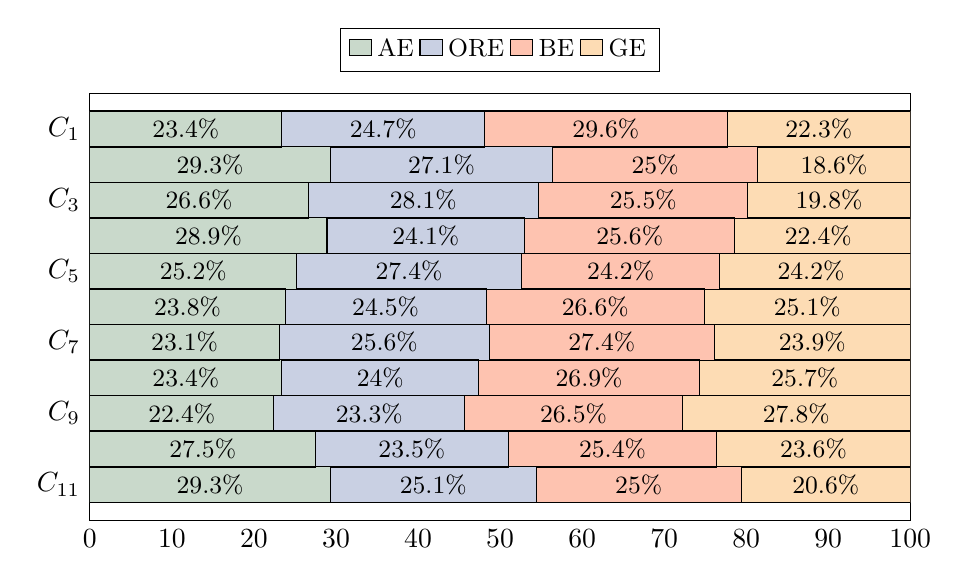
\begin{tikzpicture}  
\begin{axis}[  
    xbar stacked, % 横向堆积条形图  
    width=12cm, % 图表宽度  
    height=7cm, % 图表高度  
    xlabel style={font=\Large},
    ylabel style={font=\Large},
    legend style={font=\small},
    tick label style={font=\normalsize},
    ytick style={font=\large},
    xmin=0,
    xmax=100,
    legend style={  
        at={(0.5,1.05)}, % 图例位置  
        anchor=south,  
        legend columns=-1  
    },  
    xtick style={draw=none},
    symbolic y coords={$C_{11}$,$C_{10}$,$C_{9}$,$C_{8}$,$C_{7}$,$C_{6}$,$C_{5}$,$C_{4}$,$C_{3}$,$C_{2}$,$C_{1}$}, % y轴刻度为符号标签   
    bar width=13pt % 条形宽度  
]  
\node[anchor=center] at (axis cs:11.7,$C_{1}$) {\small 23.4\%};
\node[anchor=center] at (axis cs:35.75,$C_{1}$) {\small 24.7\%};
\node[anchor=center] at (axis cs:62.9,$C_{1}$) {\small 29.6\%};
\node[anchor=center] at (axis cs:88.85,$C_{1}$) {\small 22.3\%};

\node[anchor=center] at (axis cs:14.65,$C_{2}$) {\small 29.3\%};
\node[anchor=center] at (axis cs:42.85,$C_{2}$) {\small 27.1\%};
\node[anchor=center] at (axis cs:68.9,$C_{2}$) {\small 25\%};
\node[anchor=center] at (axis cs:90.7,$C_{2}$) {\small 18.6\%};

\node[anchor=center] at (axis cs:13.3,$C_{3}$) {\small 26.6\%};
\node[anchor=center] at (axis cs:40.65,$C_{3}$) {\small 28.1\%};
\node[anchor=center] at (axis cs:67.45,$C_{3}$) {\small 25.5\%};
\node[anchor=center] at (axis cs:90.1,$C_{3}$) {\small 19.8\%};

\node[anchor=center] at (axis cs:14.45,$C_{4}$) {\small 28.9\%};
\node[anchor=center] at (axis cs:40.95,$C_{4}$) {\small 24.1\%};
\node[anchor=center] at (axis cs:65.8,$C_{4}$) {\small 25.6\%};
\node[anchor=center] at (axis cs:88.8,$C_{4}$) {\small 22.4\%};

\node[anchor=center] at (axis cs:12.6,$C_{5}$) {\small 25.2\%};
\node[anchor=center] at (axis cs:38.9,$C_{5}$) {\small 27.4\%};
\node[anchor=center] at (axis cs:64.7,$C_{5}$) {\small 24.2\%};
\node[anchor=center] at (axis cs:87.9,$C_{5}$) {\small 24.2\%};

\node[anchor=center] at (axis cs:11.9,$C_{6}$) {\small 23.8\%};
\node[anchor=center] at (axis cs:36.05,$C_{6}$) {\small 24.5\%};
\node[anchor=center] at (axis cs:61.6,$C_{6}$) {\small 26.6\%};
\node[anchor=center] at (axis cs:87.45,$C_{6}$) {\small 25.1\%};

\node[anchor=center] at (axis cs:11.55,$C_{7}$) {\small 23.1\%};
\node[anchor=center] at (axis cs:35.9,$C_{7}$) {\small 25.6\%};
\node[anchor=center] at (axis cs:62.4,$C_{7}$) {\small 27.4\%};
\node[anchor=center] at (axis cs:88.05,$C_{7}$) {\small 23.9\%};

\node[anchor=center] at (axis cs:11.7,$C_{8}$) {\small 23.4\%};
\node[anchor=center] at (axis cs:35.4,$C_{8}$) {\small 24\%};
\node[anchor=center] at (axis cs:60.85,$C_{8}$) {\small 26.9\%};
\node[anchor=center] at (axis cs:87.15,$C_{8}$) {\small 25.7\%};

\node[anchor=center] at (axis cs:11.2,$C_{9}$) {\small 22.4\%};
\node[anchor=center] at (axis cs:34.05,$C_{9}$) {\small 23.3\%};
\node[anchor=center] at (axis cs:58.95,$C_{9}$) {\small 26.5\%};
\node[anchor=center] at (axis cs:86.1,$C_{9}$) {\small 27.8\%};

\node[anchor=center] at (axis cs:13.75,$C_{10}$) {\small 27.5\%};
\node[anchor=center] at (axis cs:39.25,$C_{10}$) {\small 23.5\%};
\node[anchor=center] at (axis cs:63.7,$C_{10}$) {\small 25.4\%};
\node[anchor=center] at (axis cs:88.2,$C_{10}$) {\small 23.6\%};

\node[anchor=center] at (axis cs:14.65,$C_{11}$) {\small 29.3\%};
\node[anchor=center] at (axis cs:41.85,$C_{11}$) {\small 25.1\%};
\node[anchor=center] at (axis cs:66.9,$C_{11}$) {\small 25\%};
\node[anchor=center] at (axis cs:89.7,$C_{11}$) {\small 20.6\%};


% 设计数据,确保每个类别的三个子部分相加为100  
\addplot[fill=color1!40] coordinates {(23.4,$C_{1}$) (29.3,$C_{2}$) (26.6,$C_{3}$) (28.9,$C_{4}$) (25.2,$C_{5}$) (23.8,$C_{6}$) (23.1,$C_{7}$) (23.4,$C_{8}$) (22.4,$C_{9}$) (27.5,$C_{10}$) (29.3,$C_{11}$)}; % 第一层数据,蓝色 

\addplot[fill=color5!40] coordinates {(24.7,$C_{1}$) 
(27.1,$C_{2}$) (28.1,$C_{3}$) (24.1,$C_{4}$) (27.4,$C_{5}$) (24.5,$C_{6}$) (25.6,$C_{7}$) (24,$C_{8}$) (23.3,$C_{9}$) (23.5,$C_{10}$) (25.1,$C_{11}$)}; % 第二层数据,绿色  

\addplot[fill=color3!40] coordinates {(29.6,$C_{1}$) (25,$C_{2}$) (25.5,$C_{3}$) (25.6,$C_{4}$) (24.2,$C_{5}$) (26.6,$C_{6}$) (27.4,$C_{7}$) (26.9,$C_{8}$) (26.5,$C_{9}$) (25.4,$C_{10}$) (25,$C_{11}$)}; % 第三层数据,红色

\addplot[fill=color4!40] coordinates {(22.3,$C_{1}$) (18.6,$C_{2}$) (19.8,$C_{3}$) (22.4,$C_{4}$) (24.2,$C_{5}$) (25.1,$C_{6}$) (23.9,$C_{7}$) (25.7,$C_{8}$) (27.8,$C_{9}$) (23.6,$C_{10}$) (20.6,$C_{11}$)}; % 第三层数据,红色



\legend{AE,ORE,BE,GE} % 图例  
  
\end{axis}  
\end{tikzpicture}  
}\caption{The visualization of balanced spatial expert weights calculated in Eq.(\ref{moe_out}). The length of the bar in different colors represents the weights for the corresponding expert. $C_1$ to $C_{11}$ is different Event types in quadruples.}
\label{fig:expert}
\end{figure}  











\section{Results and Discussions}



%%分三部分,抽取,定位,分类
\subsection{Experimental Results}

Table~\ref{tab:main_results} and Table!\ref{tab:plm} shows the performance comparison of different models on our M-VAE task, and we can see that: \textbf{For extraction performance}, our \textbf{Sherlock} model outperforms all baselines, with an average improvement of 10.85 ($p$-value < 0.05) over the second performance. Specifically, our \textbf{Sherlock} model surpasses the second performance by an average of 9.9 ($p$-value < 0.05), 8.59 ($p$-value < 0.05), and 9.52 ($p$-value < 0.05) in average Single, Pair, and Quadruple metrics, justifying the effectiveness of \textbf{Sherlock} on extraction task. 
\textbf{For localization performance},
our \textbf{Sherlock} model exceeds the second performance by 11.42 ($p$-value < 0.01) in average mAP@tIoU metric, justifying the effectiveness of \textbf{Sherlock} on localization task.  Furthermore, \textbf{for classification performance}, in FNRs and F2 metric, \textbf{Sherlock} surpasses the second performance in 18.38 ($p$-value < 0.01) and 14.43 ($p$-value < 0.01). This implies the importance of our global and local information and justifies the effectiveness of our \textbf{Sherlock} model on our task.




\begin{figure}[t]
\setlength{\abovecaptionskip}{1 ex}
\setlength{\belowcaptionskip}{-1 ex}
  \centering
  \includegraphics[width=\columnwidth]{image/bar6943.pdf}
  \caption{(a) is the visual comparison of our SIR and (b) is the comparison of the average inference time for a one-minute video between Sherlock and other Video-LLMs.}
  \Description{our model xxx}
  \label{fig:infertime}
  
\end{figure}

\begin{table}[]
\setlength{\belowcaptionskip}{-1 ex}
\caption{Comparison of localization and anomaly classification task with several well-performing non-LLM models.}
\resizebox{\linewidth}{!}{
\begin{tabular}{c|cccc|ccc}
\hline
                           & \multicolumn{4}{c|}{\textbf{Anomaly Location}}                                                                                                                           & \multicolumn{2}{c}{\textbf{Anomaly Cls.}}                                   \\ \cline{2-7} 
                           &                                       & \multicolumn{2}{c}{mAP@tIoU}                                                  &                                       &                                       &                                       \\ \cline{3-4}
\multirow{-3}{*}{\textbf{Models}} & 0.1                                   & 0.2                                   & 0.3                                   & \multirow{-2}{*}{Average}             & \multirow{-2}{*}{FNRs}                & \multirow{-2}{*}{F2}                  \\ \hline
BiConvLSTM\cite{tab45}                 & 52.74                                 & 37.31                                 & 31.12                                 & 40.39                                 & 68.05                                 & 44.48                                 \\
SPIL\cite{tab44}                       & 53.28                                 & 38.89                                 & 32.91                                 & 41.69                                 & 67.84                                 & 46.87                                 \\
FlowGatedNet\cite{tab43}               & 53.64                                 & 39.64                                 & 33.18                                 & 42.15                                 & 67.24                                 & 46.55                                 \\
X3D\cite{tab42}                        & 54.52                                 & 40.05                                 & 34.96                                 & 43.17                                 & 65.08                                 & 48.65                                 \\
HSCD\cite{tab41}                      & 56.14                                 & 42.87                                 & 35.28                                 & 44.76                                 & 60.36                                 & 52.28                                 \\ \hline
\rowcolor{lightpink} \textbf{Sherlock}          & {\color[HTML]{3166FF} \textbf{94.03}} & {\color[HTML]{3166FF} \textbf{82.59}} & {\color[HTML]{3166FF} \textbf{76.12}} & {\color[HTML]{3166FF} \textbf{84.24}} & {\color[HTML]{3166FF} \textbf{17.24}} & {\color[HTML]{3166FF} \textbf{83.59}} \\ \hline
\end{tabular}}
\label{tab:plm}
\end{table}

% \textbf{3)} Influenced by the evaluation model proposed by Video-Bench~\cite{video-bench}, we used T5-based and GPT-based evaluation metrics to evaluate the extraction ability of \textbf{Sherlock} and other models. The average improvement of other models is \textbf{23.09}, while we are \textbf{17.84} ($p$-value < 0.01). This indicates that \textbf{Sherlock} can follow the instructions well and extract quadruples that meet our requirements.

\begin{figure*}[t]
\vspace{-0.3cm}
\setlength{\abovecaptionskip}{0.5 ex}
\setlength{\belowcaptionskip}{-3 ex}
  \centering
  \includegraphics[width=\textwidth]{image/case.pdf}
  \caption{Two Visualized samples to compare Sherlock with other Video-LLMs.}
  \Description{our model xxx}
  \label{fig:casestudy}
\end{figure*}

\subsection{Contributions of Each Key Component}
In order to further investigate the contributions of different modules of \textbf{Sherlock}, we conduct an ablation study on our \textbf{Sherlock} model. As shown in Table~\ref{tab:main_results}, w/o AE, w/o ORE, w/o BE, w/o GE, w/o EG, and w/o pre-tuning represent without four Spatial Experts, Expert Gate, and pre-tuning stage in sec~\ref{3.3} respectively.








\textbf{Effectiveness Study of Global and Local Spatial Expert}. From Table~\ref{tab:main_results}, we can see that: The performance of \textbf{w/o AE}, \textbf{w/o ORE}, \textbf{w/o BE} and \textbf{w/o GE} degrades in all metrics, with an average decrease of 7.54 ($p$-value < 0.01), 7.57 ($p$-value < 0.01), 4.37 ($p$-value < 0.01), and 5.68 ($p$-value < 0.01) in FNRs, F2, average map@tIoU, and average event extraction metrics. This confirms the importance of global and local information in extracting and localizing abnormal events, and \textbf{Sherlock} can better model those information well.



\textbf{Effectiveness Study of Spatial Imbalance Regulator.} From Table~\ref{tab:main_results}, we can see that: \textbf{1)} Compared with \textbf{Sherlock}, \textbf{w/o EG} shows poorer performance in all metrics, with a decrease of FNRs, F2, average map@tIoU, and average extraction performance by 15.34 ($p$-value < 0.01), 16.52 ($p$-value < 0.01), 8.62 ($p$-value < 0.05) and 10.36 ($p$-value < 0.01), respectively. This demonstrates the effectiveness of GSM in global-local spatial modeling and encourages us to consider handling heterogeneity issues between spatial information in the manner of MoE. 
\textbf{2)} From Table~\ref{tab:main_results}, we can see that compared to performance of \textbf{w/o SIR}, the performance of \textbf{w/o MG} is poorer, with FNRs, F2, average map@tIoU, and average event extraction metrics decreasing by 1.94 ($p$-value < 0.05), 3.9 ($p$-value < 0.05), 1.13 ($p$-value < 0.05) and 4.84 ($p$-value < 0.05), respectively. This further demonstrates the effectiveness of $\mathcal{L}_\text{gate}$ in global-local spatial balancing and encourages us to consider using SIR to better balance spatial information. 
\textbf{3)} In addition, we record the weights of four spatial experts after training in Figure~\ref{fig:expert} and Figure~\ref{fig:infertime} (a). We can see that the weights of all experts have been relatively balanced, and each expert has demonstrated outstanding professional abilities when facing different types of abnormal videos.




% \begin{table}[]
% \setlength{\belowcaptionskip}{-1 ex}
% \caption{Comparison of localization and anomaly classification task with several well-performing non-LLM models which is conducted on publicly available datasets.}
% \resizebox{\linewidth}{!}{
% \begin{tabular}{c|cccc|ccc}
% \hline
%                            & \multicolumn{4}{c|}{\textbf{Anomaly Location}}                                                                                                                           & \multicolumn{2}{c}{\textbf{Anomaly Cls.}}                                   \\ \cline{2-7} 
%                            &                                       & \multicolumn{2}{c}{mAP@tIoU}                                                  &                                       &                                       &                                       \\ \cline{3-4}
% \multirow{-3}{*}{\textbf{Models}} & 0.1                                   & 0.2                                   & 0.3                                   & \multirow{-2}{*}{Average}             & \multirow{-2}{*}{FNRs}                & \multirow{-2}{*}{F2}                  \\ \hline
% BiConvLSTM\cite{tab45}                 & 52.74                                 & 37.31                                 & 31.12                                 & 40.39                                 & 68.05                                 & 44.48                                 \\
% SPIL\cite{tab44}                       & 53.28                                 & 38.89                                 & 32.91                                 & 41.69                                 & 67.84                                 & 46.87                                 \\
% FlowGatedNet\cite{tab43}               & 53.64                                 & 39.64                                 & 33.18                                 & 42.15                                 & 67.24                                 & 46.55                                 \\
% X3D\cite{tab42}                        & 54.52                                 & 40.05                                 & 34.96                                 & 43.17                                 & 65.08                                 & 48.65                                 \\
% HSCD\cite{tab41}                      & 56.14                                 & 42.87                                 & 35.28                                 & 44.76                                 & 60.36                                 & 52.28                                 \\ \hline
% \rowcolor{lightpink} \textbf{Sherlock}          & {\color[HTML]{3166FF} \textbf{94.03}} & {\color[HTML]{3166FF} \textbf{82.59}} & {\color[HTML]{3166FF} \textbf{76.12}} & {\color[HTML]{3166FF} \textbf{84.24}} & {\color[HTML]{3166FF} \textbf{17.24}} & {\color[HTML]{3166FF} \textbf{83.59}} \\ \hline
% \end{tabular}}
% \label{tab:plm}
% \end{table}



\textbf{Effectiveness Study of Pre-tuning}. From Table~\ref{tab:main_results}, we can see that \textbf{w/o pre-tuning}, the performance is inferior to \textbf{Sherlock}. FNRs, F2, average map@tIoU, and average event extraction metrics have decreased by 17.63 ($p$-value < 0.01), 16.95 ($p$-value < 0.01), 10.92 ($p$-value < 0.01) and 11.48 ($p$-value < 0.01), respectively. This further justifies the effectiveness of pre-tuning, as well as encourages us to use more high-quality datasets to enhance the spatial understanding ability of Video-LLMs before instruction-tuning. 





\subsection{Convergence Analysis and Practical Assessment for Sherlock}
In order to analyze the convergence of Sherlock, we record the loss of baseline Video-LLMs, Sherlock, and its variant without specific components over various training steps. The results are shown in Figure~\ref{fig:train} and we can see that: \textbf{1)} \textbf{Sherlock} demonstrates the fastest convergence compared to other Video-LLMs. At the convergence point, the loss of Sherlock is 1.05, while Video-LLaVA is 2.06. This underscores the high efficiency of Sherlock over other advanced Video-LLMs. \textbf{2)} \textbf{Sherlock} demonstrates the fastest convergence compared to its variant without specific components in Figure~\ref{fig:train}. This justifies that the spatial information along with GSM and SIR can accelerate the convergence process, which further encourages us to consider the spatial information in the M-VAE task. 

To assess practicality, we analyze the FNRs of Sherlock for each scene. As shown in Table~\ref{tab:scene}, we can observe that in every scene, Sherlock outperforms other Video-LLMs. This indicates that the possibility of misclassifying abnormal events as normal events is minimized, thereby demonstrating the importance of global and local spatial modeling of Sherlock. We also analyze the average inference time in seconds for a one-minute video. As shown in Figure~\ref{fig:infertime} (b), Sherlock does not
perform much differently from the other models in terms of inference time. This is reasonable, as some studies confirm that the MoE architecture can improve efficiency [11, 28]. This suggests that introducing more information along with a MoE module for the M-VAE task does not increase the inference time and Sherlock can maintain good inference efficiency.

% \subsection{Compared with Advanced Non-LLM Models on Public Dataset}
% In order to more comprehensively evaluate the effectiveness of Sherlock, we compare our \textbf{Sherlock} model with other advanced non-LLM models~\cite{tab41,tab42,tab43,tab44,tab45} on traditional anomaly localization and anomaly classification task based on publicly available CUVA datasets~\cite{cuva}. Specifically, we need Sherlock to determine whether each second of the video is abnormal or not without generating quadruples. As shown in Table~\ref{tab:plm}, non-LLM models not only underperform relative to other Video-LLMs presented in Table~\ref{tab:plm} but also significantly inferior to our Sherlock model. This
% further demonstrates the importance of the global and local spatial information we proposed for the M-VAE task.


\subsection{Qualitative Analysis for Sherlock}
As shown in Figure~\ref{fig:casestudy}, we visualize and compare \textbf{Sherlock} with other Video-LLMs. We randomly select two samples from our dataset and ask these models to \emph{Analyze the following video and localize the timestamp and extract the quadruple of the abnormal events}. From the figure, we can see that: \textbf{1)} Accurately localizing abnormal events and extracting correct quadruples is a huge challenge. For instance, example 2 captures a segment from 9s to 15s, where identifying the collision of the truck at road is challenging, \textbf{2)} Compared with other advanced Video-LLMs, \textbf{Sherlock} shows excellent performance in localizing abnormal events. In example 1, \textbf{Sherlock} outperforms other models in terms of accuracy. In example 2, it outperforms PandaGPT in terms of accuracy and can generate a correct quadruple. This further demonstrates the effectiveness of \textbf{Sherlock} in precisely extracting and localizing abnormal events.
Software development is increasingly conceived as a collaboration activity between developers and AIs. Indeed, IDEs already implement features to enable interactive development, with AI suggesting implementations that are reused by developers.

Although multiple studies show this interaction can be successful, there is still limited understanding of how the models must be configured and used in the context of code generation tasks. This study addresses this gap, systematically investigating the impact of several key parameters, including the repeated submission of a prompt to accommodate for the non-deterministic nature of the models.

Our study reveals several key findings about the usage of ChatGPT. In particular, we discovered how creativity, although up to a limited extent, is useful to increase the range of methods whose code can be generated correctly. A major role is played by parameter top-p, which is commonly underrated, and instead has a major impact on the correctness of the results, with lower values producing better results. Finally, prompts should be submitted multiple times, with $5$ repetitions combined with a temperature of $1.2$ resulting in an effective configuration in our experiments.  

Future work concerns two main research directions. One is about replicating this experiment with other AI assistants, to validate our findings in multiple contexts. The second research direction concerns finding strategies to deal with the need to submit the same prompt multiple times to obtain a useful result, and thus developing approaches able to select or merge multiple responses automatically. 

\begin{acks}
We thank our anonymous reviewers for their helpful comments. This work was supported by three NSFC grants, i.e., No.62006166, No.62376178 and No.62076175. This work was also supported by a Project Funded by the Priority Academic Program Development of Jiangsu Higher Education Institutions (PAPD).
\end{acks}

\bibliographystyle{ACM-Reference-Format}
\bibliography{sample-base}




\end{document}
\endinput
%%
%% End of file `sample-sigconf-authordraft.tex'.
